\documentclass[12pt, a4paper,oneside, openany]{book}
%fuente12pt,tamaño carta,una cara,quitar hojas en blanco,tipo libro
\usepackage[utf8]{inputenc} %fuente Unicode
%\usepackage[margin=-0cm]{geometry} %margen
\usepackage{graphicx} %uso de imagenes
\usepackage{multicol} %uso de multicolumnas
\usepackage{multirow} %multi celdas
\usepackage{lastpage} %n.total de paginas
\usepackage{colortbl} %columnas de color
\usepackage{tikz, tikz-3dplot} %figuras
\usepackage{tkz-euclide}
\usepackage{adjustbox} %manejo de margenes
\usepackage[spanish]{babel} %lenguaje español
\usepackage[document]{ragged2e} %alineacion
\usepackage[T1]{fontenc} %codificacion fuente
\usepackage{enumerate} %viñeta numeros
\usepackage{palatino} %fuente
\usepackage[colorlinks,linkcolor=myblue,citecolor=mygreen]{hyperref} %link personalizado
\usepackage{tabularx}
%-----------------------------------------------------------------
\definecolor{myblue}{HTML}{2D74B5} %color de titulos y subtitulos
%-----------------------------------------------------------------
\graphicspath{ {img/} } %localizacion de carpeta con imagenes
\renewcommand{\baselinestretch}{1.2} %espacio entre parrafos

%\AtBeginDocument{\AtBeginShipoutNext{\AtBeginShipoutDiscard}}
%elimina paginas adicionales que se agregan con el uso de hyperref
\usepackage{multirow} %multi celdas en tablas
\usepackage{longtable} %tablas multipagina
\usepackage{caption} %ajuste de tablas, figuras
\usepackage{color} %colores de texto
\usepackage{wrapfig} %rodear imagenes
\usepackage{booktabs, multirow} %bordes y rangos
\usepackage{titlesec} %titulos personalizados
\usepackage{eso-pic,picture} %imagenes con texto
\usepackage{nomencl} %simbolos de nomenclatura
\usepackage{lipsum} %crea texto default
\makenomenclature %tamaño nomenclatura
%\usepackage{showframe} %muestra el margen de las pg
%-----------------------------------------------------------------
%codigo del borde
\AddToShipoutPicture{%
\setlength\fboxsep{1pt}%
\put(24pt,24pt){\framebox(19.3066cm,28.0066cm)[lb]{}}%
}

%margenes
\usepackage{geometry}
\newgeometry{
        top=0.001in,
        bottom=3.2in,
        outer=0.55in,  %izquierda
        inner=0.55in, %derecha
        }
%-----------------------------------------------------------------
\usepackage{fancyhdr}%uso de encabezado y pie personalizado
\pagestyle{fancy}
\fancyhf{}%Declaración de encabezado
\renewcommand\headrulewidth{0pt}
\fancypagestyle{plain}{}%encabezado general


\setlength{\headheight}{160pt}%ubicacion de caja de encabezado

\titlespacing{\chapter}{0pt}{-42pt}{0.5cm}%config capitulos, espacio de chapter
\titleformat{\chapter}[display]
{\sffamily\color{myblue}} {
    {\normalfont\color{myblue}\Large}
        \hspace{0pt}
            {\setlength\fboxsep{0pt}
                \colorbox{myblue}{
                }
            }
    }
{0 pt}
{\titlerule[0pt]\LARGE\sffamily}

%%%%%%%%%%%%%%%%%%%%%%%%%%%%%%%%%%%%%%%%%%%%%%%%%%%%%%%%%%%%%%%%%%%%%%%

\lhead{

\begin{minipage}{0.1\textwidth}
\scalebox{1}[1.2]{
\begin{tabular}{|m{2cm}|m{10.8cm}|m{1.0cm}|m{1.0cm}|m{1.0cm}| }

\hline

\multirow{3}{2cm}{\centering
\includegraphics[width=0.88\textwidth]{tjacdmx_logo.png}}
& \footnotesize\centering\bf\sffamily{TRIBUNAL DE JUSTICIA ADMINISTRATIVA DE TABASCO}
& \footnotesize\bf\sffamily{Día}
& \footnotesize\bf\sffamily{Mes}
&\footnotesize\bf\sffamily{Año}
\\ \cline{2-5}

& \centering\bf\footnotesize\sffamily{DIRECCIÓN GENERAL DE ADMINISTRACIÓN}
& \footnotesize\bf\sffamily{27}
& \footnotesize\bf\sffamily{02}
& \footnotesize\bf\sffamily{2023}
\\ \cline{2-5}

& \centering\bf\footnotesize\sffamily{DIRECCIÓN DE INFORMÁTICA}
& \multicolumn{3}{ |c| }{\bf\footnotesize\sffamily{Versión: 102 }}
\\ \cline{2-5}

&
\centering\bf\footnotesize\sffamily{MANUAL DE USUARIO}
& \multicolumn{3}{ |c| } {\bf\footnotesize\sffamily{Página \thepage~de\ \pageref{LastPage}}}
\\ \hline

\end{tabular}}
\end{minipage}

}

%-------------------------------------------------------------------
%pie de todas las paginas
\cfoot{
            \makebox[\textwidth][c]{
				\footnotesize\sffamily
                \begin{tabular}{ |m{4cm}|m{4cm}|m{4cm}|m{4cm}| }
                    \hline
                    {\bf IDENTIFICACIÓN}
                    & {\bf ELABORÓ}
                    & {\bf REVISÓ}
                    & {\bf AUTORIZÓ} \\
                    \hline
                    {\scriptsize TJACDMX/DI/SIDJ/Actuaria/V3}
                    & Programador
                    & Jefe de unidad departamental
                    & Dirección de informática \\ 
                    \hline
                \end{tabular}
            }
}

%-----------------------------------------------------------------
\begin{document}%inicio de documento

%-----------------------------------------------------------------

\centerline{
\includegraphics[width=0.8\textwidth]{tjacdmx_logo.png}}%imagen de logo en portada
%titulo de portada

\vspace{1cm}%espacio
%-----------------------------------------------------------------
\begin{flushright}%alineación a la derecha

\newcommand{\ProjectTitle}

\vspace{0cm}
%titulo en portada
{\color{myblue}{\sffamily\large\bf\sffamily
ACTUARIA V3.0 \\
MANUAL DE USUARIO\\
\vspace{0.3cm}
DIRECCIÓN DE INFORMÁTICA}
}
\end{flushright}
%-----------------------------------------------------------------

\newpage
\begin{center}
\begin{tabular}{| c | c | c | c |} 
\hline
\multicolumn{4}{ | c | }{\cellcolor[gray]{0.9}CONTROL DE VERSIONES} \\ 
\hline 
Versión &               Elaborado por:          & Fecha de última modificación          & Motivo \\ 
\hline
1.0.1   & Esthefania Vidal Solares        &      12/octubre/2022 & Creación \\ 
\hline
1.0.2   & Esthefania Vidal Solares        &     27/febrero/2023 & Actualización  \\ 
\hline
\end{tabular}
\end{center}

\renewcommand{\headrulewidth}{0pt}%sin linea por default

\tableofcontents

\chapter{\large{Objetivo}}\label{chap:objetivo}
Con la finalidad de ofrecer a los servidores públicos del Tribunal de Justicia Administrativa de Tabasco,
herramientas que coadyuven en la operación de los apartados que integran el módulo
de «Actuaría v 3.0», se elaboró el presente Manual.

%-----------------------------------------------------------------
% Matriz de Seguridad
%-----------------------------------------------------------------
\chapter{\large{Matriz de seguridad}}\label{chap:ingreso}
\begin{center}
\begin{tabular}{| c | c | c | c | c} \hline
 \cellcolor[gray]{0.9} \bf Roles 
 &\cellcolor[gray]{0.9} \bf Lectura 
 &\cellcolor[gray]{0.9} \bf Escritura 
 &\cellcolor[gray]{0.9} \bf Borrar  \\  \hline
 Admin & X & X & X \\  \hline
 Actuario SO & X & X & X \\  \hline
 Actuario SGA & X & X & X \\ \hline
\end{tabular}
\end{center}

\chapter{\large{Acceso al módulo Actuaría v3.0}}\label{chap:ingreso}
1.Ingresaremos al Sistema Digital de Juicios, a través del siguiente enlace:

\begin{center}
\href{https://sidj.tjacdmx.gob.mx}{https://sidj.tjacdmx.gob.mx}
\end{center}

2.Ubicaremos en el menú principal y daremos click en  el correspondiente a {\bf{
<<Actuaria v3.0>> }}

\begin{center}
    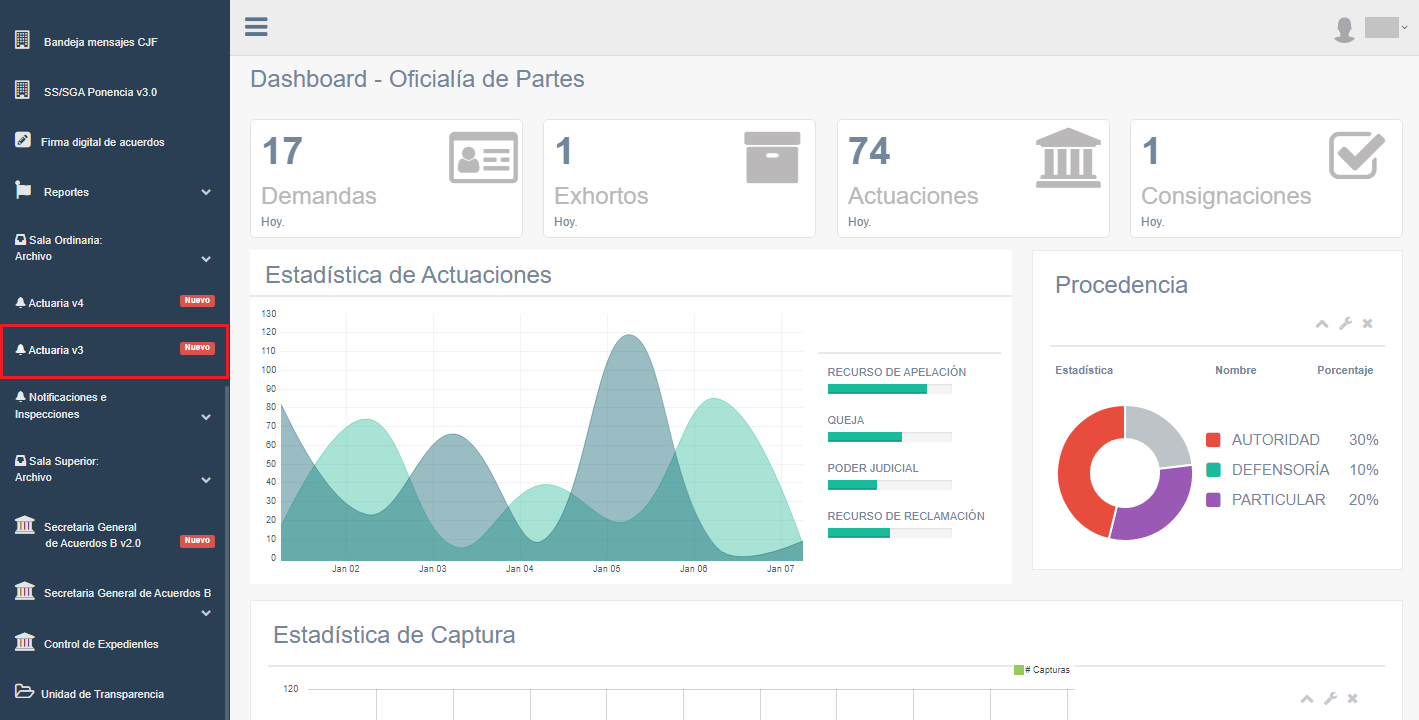
\includegraphics[width=0.88\columnwidth]{inicioAc.png}
\end{center}

\chapter{\large{ Consulta de expediente y notificaciones.}}\label{chap:consulta}

En el menú: {\bf Consulta de expediente y notificaciones}, podrá realizar las siguientes actividades:

\begin{itemize}
    \item Buscar expediente.
    \item Consulta de notificación.
    \item Subir notificación.
    \item Visualizar notificación.
    \item Editar notificación.
    \item Eliminar notificación.
    \item Buscar notificación.
\end{itemize}


1. Formas de buscar un expediente.
\begin{center}
    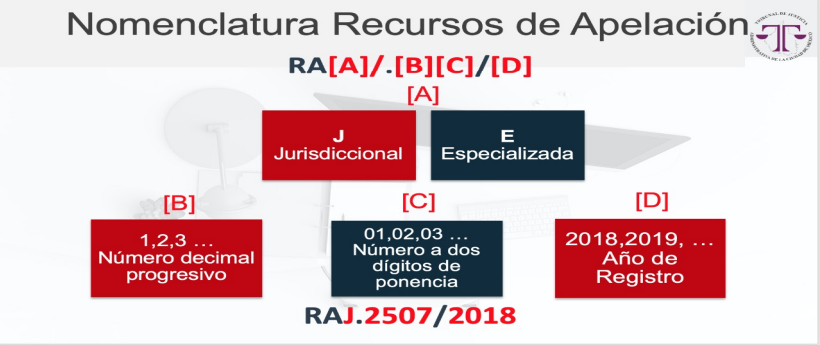
\includegraphics[width=0.88\columnwidth]{C1.png}
    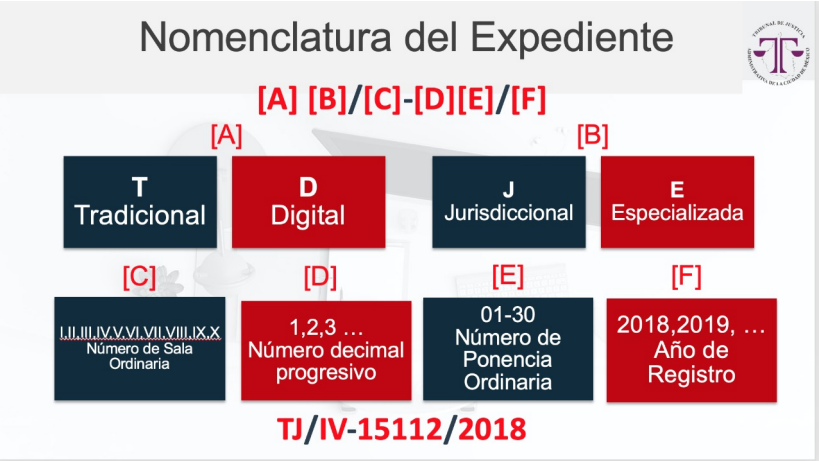
\includegraphics[width=0.88\columnwidth]{C2.png}
\end{center}

Ejemplos:
\begin{itemize}
    \item TJ/I-01/2018.
    \item -01/2018.
    \item RAJ.2507/2018.
    \item .2507/2018.
\end{itemize}

2. ¿Cómo se consulta un expediente?\\
Una vez que haya ingresado, a la opción {\bf «Consulta de expediente»}, verá una pantalla como la
siguiente, con los elementos mencionados a continuación:

\begin{center}
    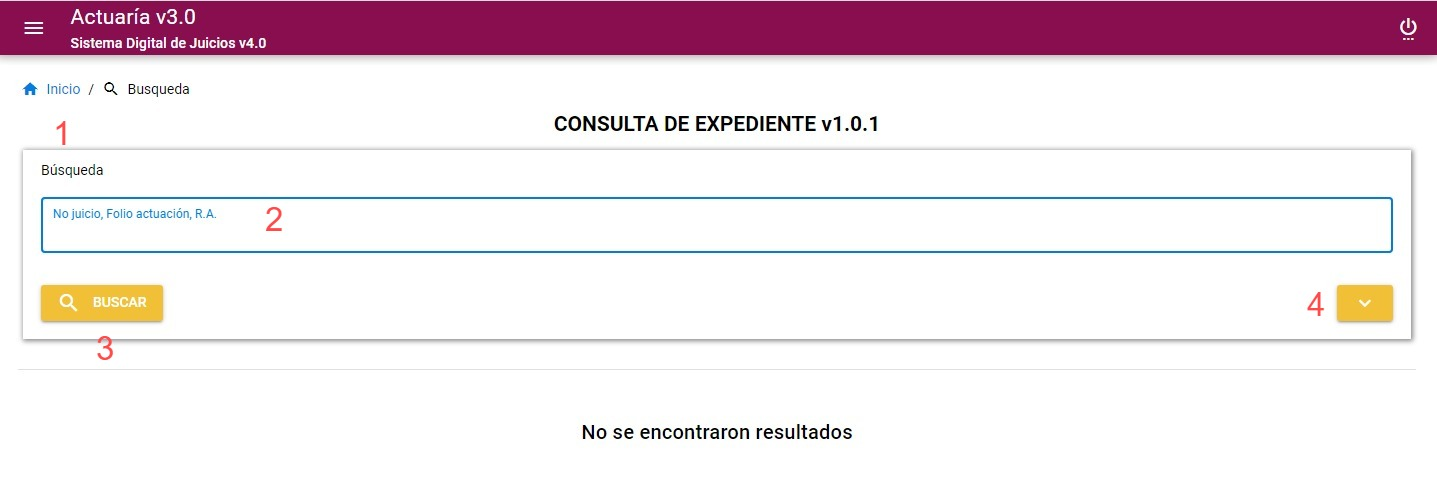
\includegraphics[width=0.88\columnwidth]{consulta.jpeg}
\end{center}
\begin{itemize}
    \item {\bf «Inicio»} podrá regresar en cualquier momento a la pantalla de principal de la aplicación. \\
    \item {\bf No. juicio}: en esta opción deberá ingresar el número de expediente para realizar la búsqueda. \\
    \item {\bf BUSCAR} mostrará los resultados coincidentes. \\
    \item {\bf BÚSQUEDA AVANZADA}: despliega filtros complementarios para la búsqueda. \\
\end{itemize}

\begin{center}
    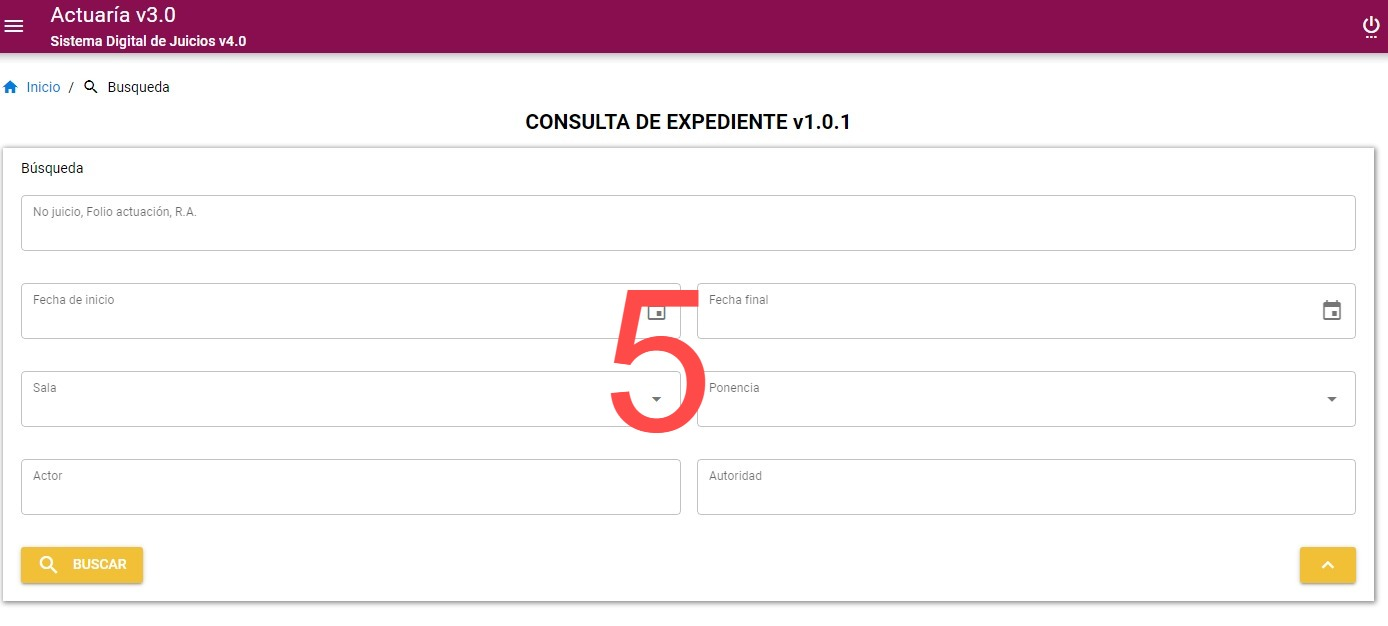
\includegraphics[width=0.88\columnwidth]{avanzada.jpeg}
\end{center}

5. Para realizar una búsqueda avanzada deberá contar con al menos uno de los siguientes
datos:
\begin{itemize}
    \item Sala. \\
    \item Ponencia. \\
    \item Actor. \\
    \item Autoridad. \\
    \item Fecha de inicio(ingreso de la actuación). \\
    \item Fecha final(Ingreso de la actuación). \\
\end{itemize}

\begin{center}
    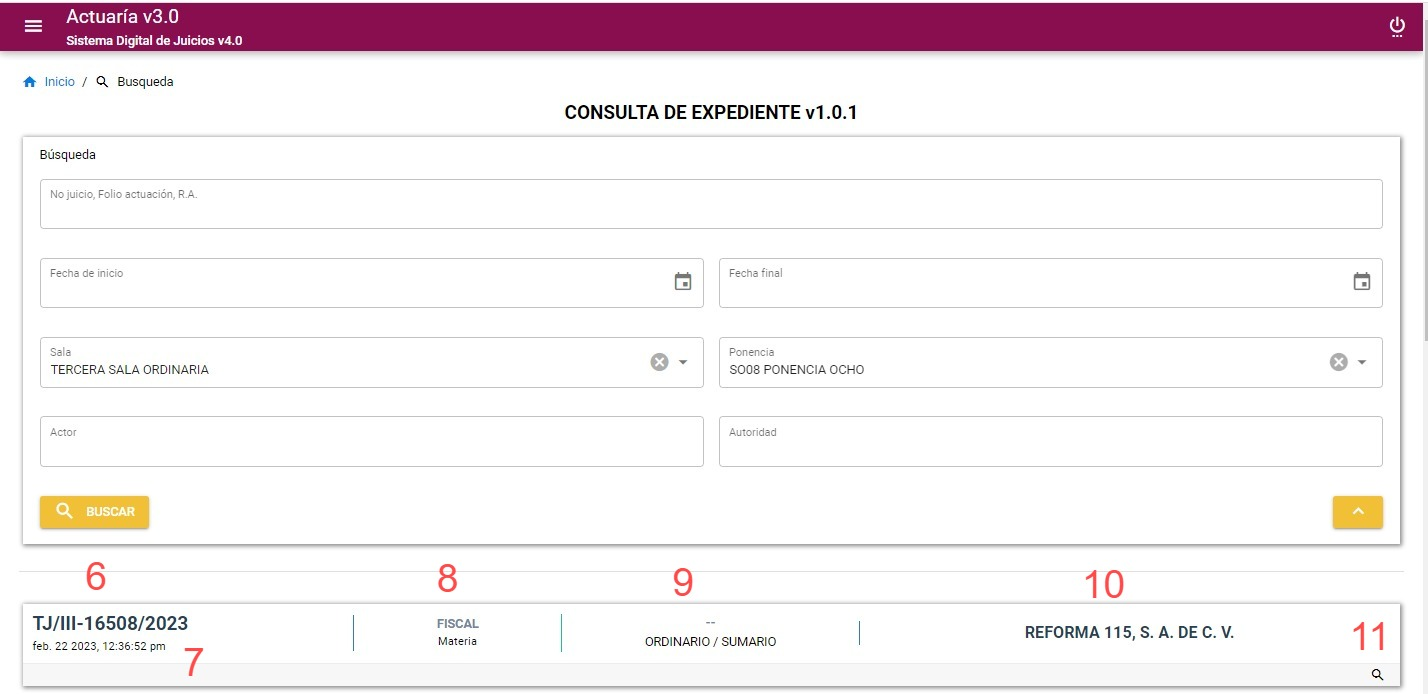
\includegraphics[width=0.88\columnwidth]{avanzada1.jpeg}
\end{center}

Una vez ingresado los datos para la búsqueda deberá dar click el botón {\bf «BUSCAR»}, el cual desplegará
los resultados coincidentes, con la descripción de los elementos referidos a continuación:

\begin{itemize}
    \item 6. Número de juicio.
    \item 7. Fecha ingreso.
    \item 8. Materia.
    \item 9. Ordinario/ Sumario.
    \item 10. Actor.
    \item 11. Consultar.
\end{itemize}

Para poder ver toda la información del expediente es necesario dar click en consultar, como se
muestra en la descripción anterior número 11, el cual presentará la siguiente pantalla.
Donde se podrá encontrar toda la información del expediente, a continuación, se describe los
elementos referidos a la consulta de expediente.

\begin{center}
    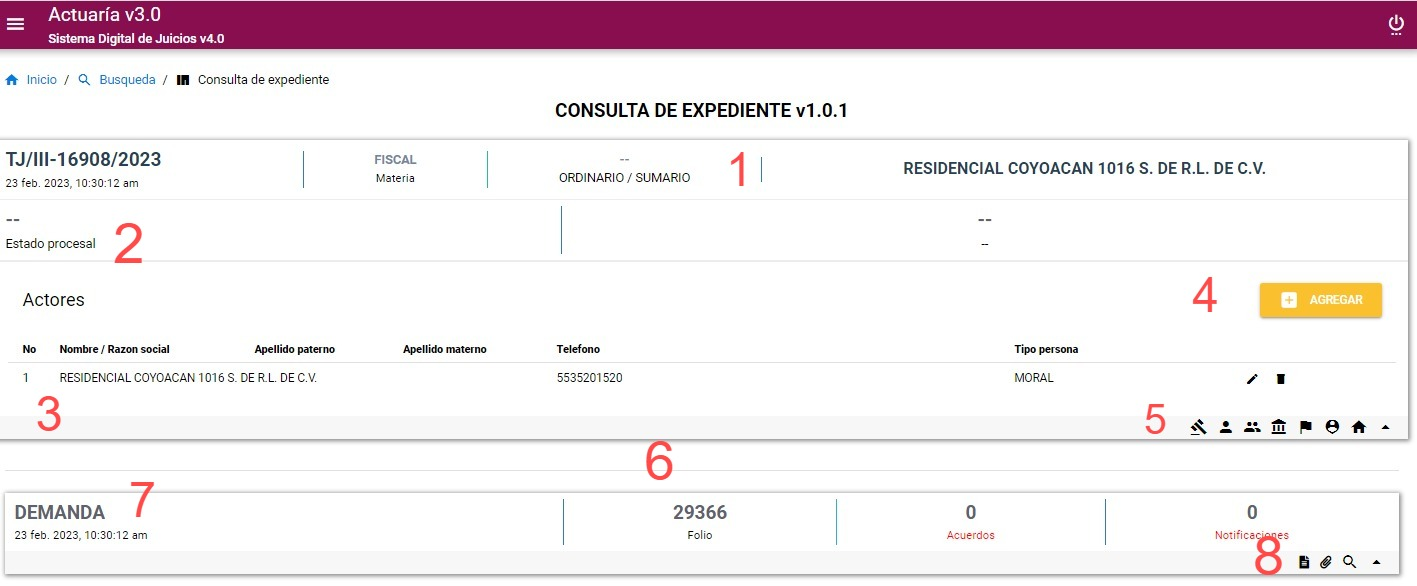
\includegraphics[width=0.88\columnwidth]{consulta_exp.jpeg}
\end{center}

\begin{enumerate}

	\item Contenedor con Información de expediente:

	\begin{itemize}
	    \item Número de juicio.
    	\item Fecha.
	    \item Materia.
    	\item Ordinario/Sumario.
	    \item Actor.
	\end{itemize}

	\item Estado procesal.

	\item Información complementaria de las secciones enumerdas en la opción {\bf 5}.

	\item Agregar.

	\item Iconos contenedores de expediente:
		\begin{itemize}
	    \item Ponencia.
    	\item Actores.
	    \item Terceros perjudicados.
	    \item Autoridades.
	    \item Representantes.
	    \item Autorizados.
	    \item Domicilio.
	\end{itemize}

	\item Muestra la lista de actuaciones que tiene el expediente.

	\item Contenedor de la actuación con la siguiente información:
		\begin{itemize}
		    \item Tipo de proceso.
		    \item Fecha.
		    \item Folio.
		    \item Número de acuerdo.
		    \item Número de notificaciones.
		\end{itemize}

	\item Iconos contenedor actuaciones:
		\begin{itemize}
		    \item Promociones.
		    \item Anexos.
		    \item Consultar.
		\end{itemize}
\end{enumerate}

\newpage

{\Huge{\color{myblue} \section{¿Cómo consultar una notificación?}\label{sec:1}}}

Es necesario dar click al icono {\bf «Consultar»} ubicado en el {\bf número “8”}, descrito anteriormente para
que pueda consultar una notificación.\\
Se mostrarán los datos de la notificación, de click en el icono {\bf {<<Visualizar>>}} ubicado en el {\bf{número ''1''}}.

\begin{center}
    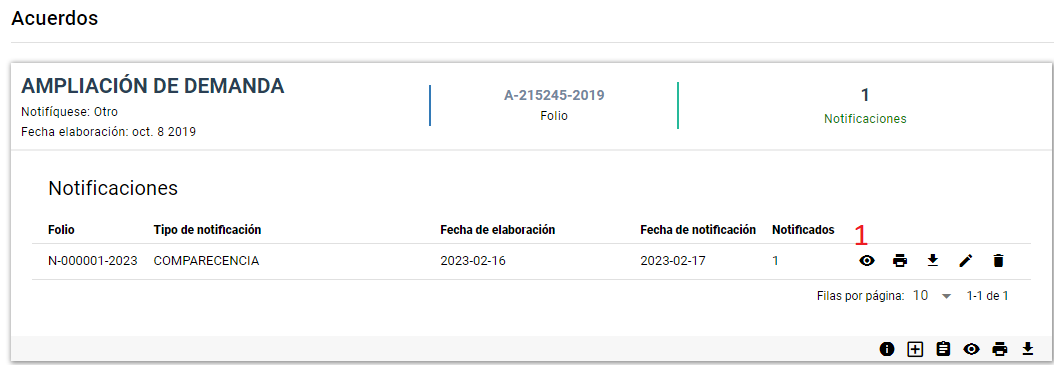
\includegraphics[width=0.88\columnwidth]{consultar_notificacion.png}
\end{center}

Se abrirá una ventana mostrando el documento.

\begin{center}
    
\includegraphics[width=0.20\columnwidth]{documento.png}
\end{center}

{\Huge{\color{myblue} \section{¿Cómo registrar una notificación?}\label{sec:2}}}

Es necesario dar click en el icono {\bf«Consultar»} ubicado en el {\bf número 8}, descrito anteriormente para
que pueda subir una notificación. A continuación, se describe:

\begin{center}
    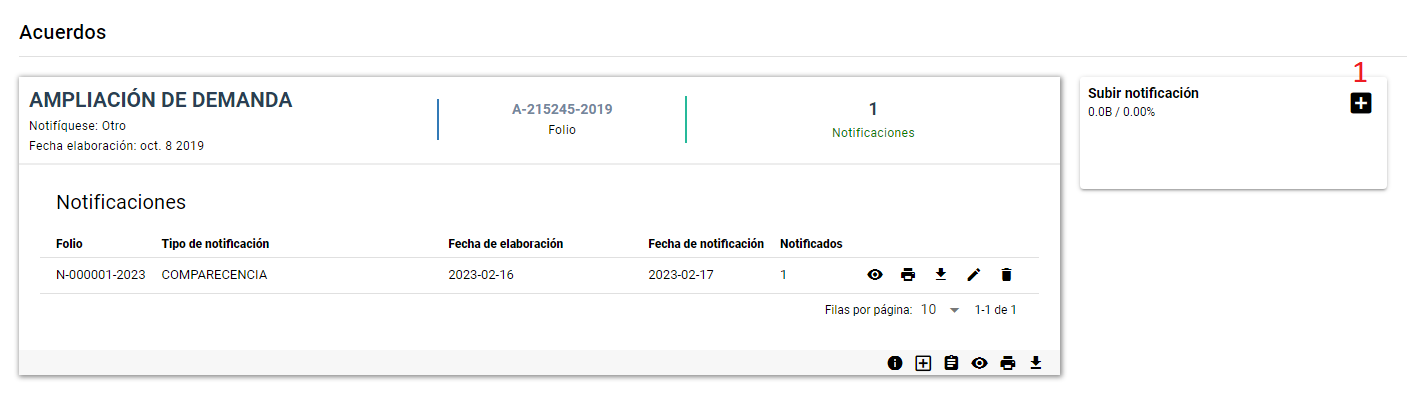
\includegraphics[width=0.88\columnwidth]{subir_notificacion.png}
\end{center}

De click en el icono ubicado con el {\bf{ número 1}} podrá seleccionar el archivo donde este guardado el documento, 
una vez que seleccione el documento, deberá dar click el botón abrir que mostrará la siguiente pantalla de
{\bf{''Registro de cédulas de notificación''}}

\begin{center}
    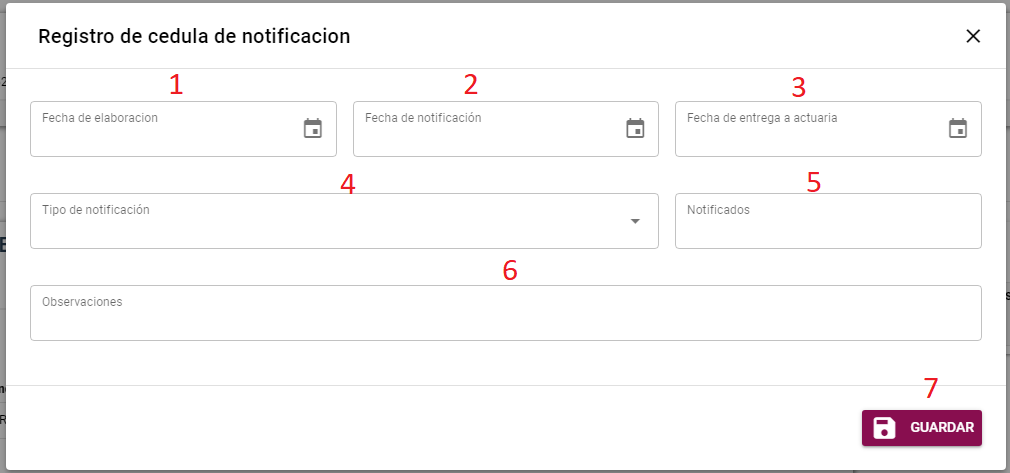
\includegraphics[width=0.55\columnwidth]{form_cedula.png}
\end{center}

Donde deberá ingresar la siguiente información:

\begin{enumerate}
    \item Fecha de elaboración.
    \item Fecha de notificación.
    \item Fecha de entrega a actuaria
    \item Tipo de notificación.
    \item Total de notificadas.
    \item Observaciones.
    \item Guardar
\end{enumerate}

Una vez capturada la información antes mencionada solo deberá dar click el botón {\bf «Guardar»}
(ubicado en el lugar {\bf “número 7”}), mostrará la notificación registrada.

{\color{myblue}\section{\normalfont\sffamily{¿Cómo editar una notificación?}}}\label{sec:3}

Es necesario dar click el icono {\bf «Consultar»} ubicado en el {\bf “número 8”}, descrito anteriormente para
que pueda editar una notificación. A continuación, se describe.

\begin{center}
    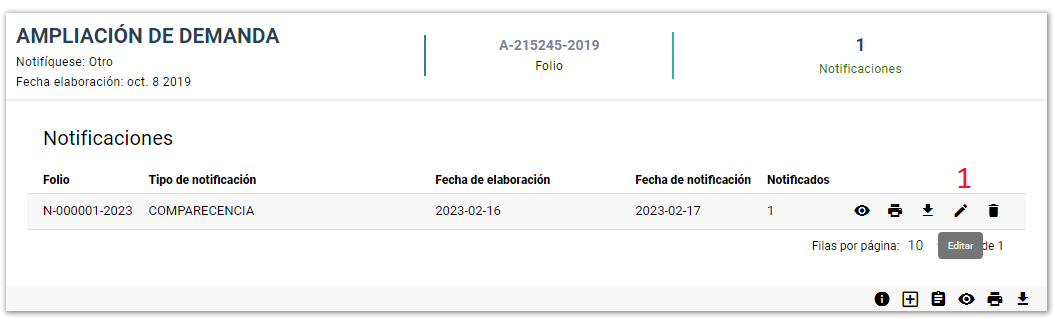
\includegraphics[width=0.88\columnwidth]{editar_notificacion.png}
\end{center}

Da click en el icono <<Editar>> indicado con el {\bf{número ''1''}} abrirá la siguiente ventana mostrando la
información de notificación.

\begin{center}
    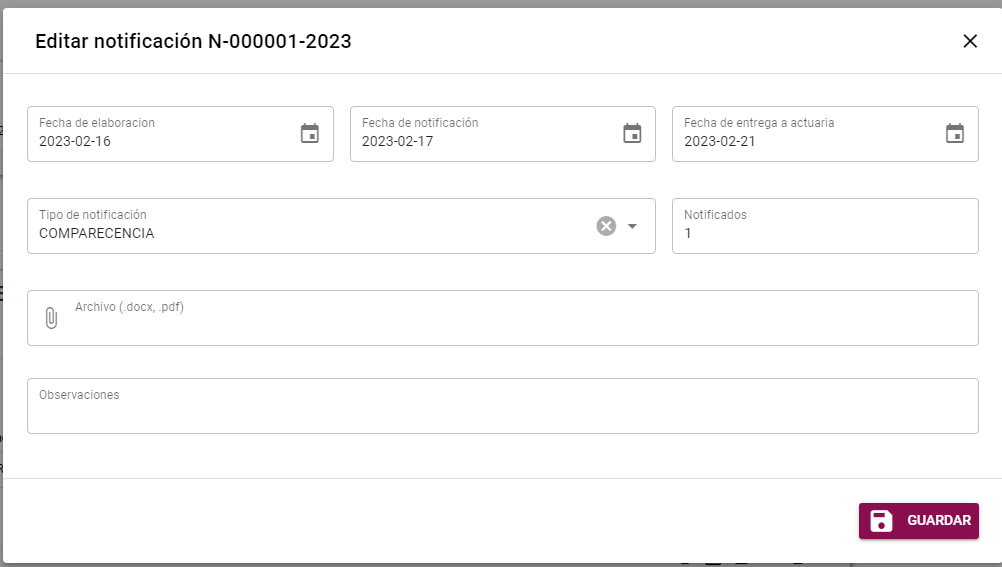
\includegraphics[width=0.65\columnwidth]{editar_not.png}
\end{center}

Podrá modificar toda la información e incluso volver a subir el archivo de notificación y podrá
guardar los cambios pulsando el botón {\bf «Guardar»}.

{\Huge{\color{myblue} \section{¿Cómo borrar una notificación?}\label{sec:4}}}

Es necesario dar click el icono «Consultar» ubicado en el “número 8”, descrito anterior-
mente para que pueda borrar una notificación. A continuación, se describe:

\begin{center}
    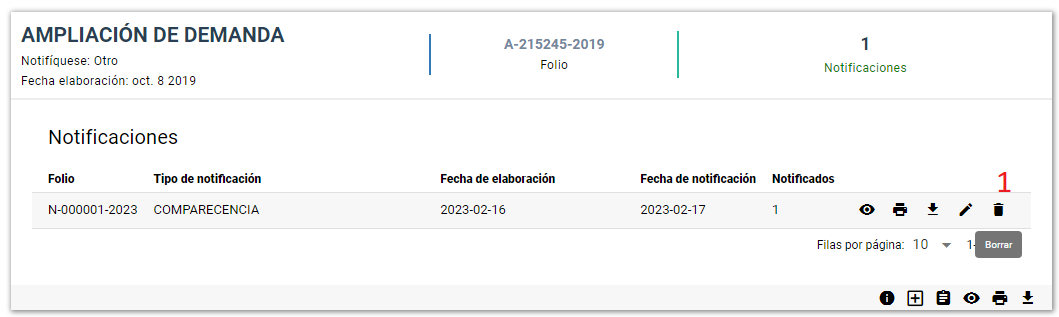
\includegraphics[width=0.65\columnwidth]{borrar_not.png}
\end{center}

Da click en el icono «Borrar» indicado con el {\bf{número ”1”}} que mostrará una ventana de advertencia.

\begin{center}
    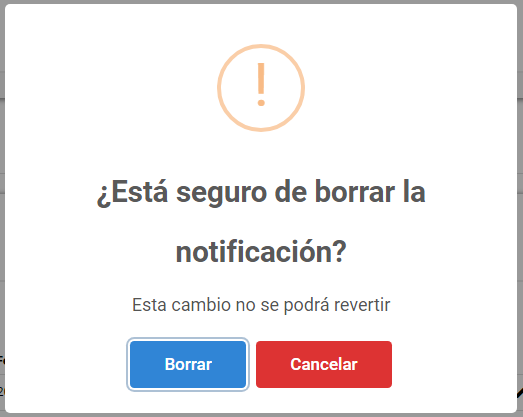
\includegraphics[width=0.33\columnwidth]{advertencia.png}
\end{center}

Sí está seguro de eliminar confirme en el botón {{\bf<<Borrar>>}} de lo contrario solo dar click en {{\bf<<Cancelar>>.}}


{\Huge{\color{myblue} \section{¿Cómo descargar una notificación?}\label{sec:5}}}

Es necesario dar click el icono {\bf{«Consultar»}} ubicado en el {\bf{“número 8”}}, 
descrito anteriormente para que pueda borrar una notificación. A continuación, se describe:

\begin{center}
    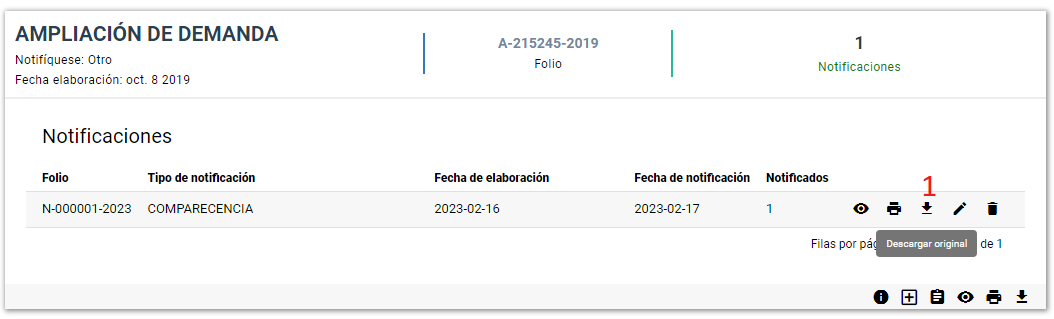
\includegraphics[width=0.88\columnwidth]{descargar_not.png}
\end{center}

Da click en el icono «Descargar» indicado con el número ”1”, y comenzará automáticamente la descarga.

\chapter{\large{Notificaciones}}\label{chap:notificaciones}

En este módulo de Notificaciones puedes realizar las siguientes acciones:
\begin{center}
    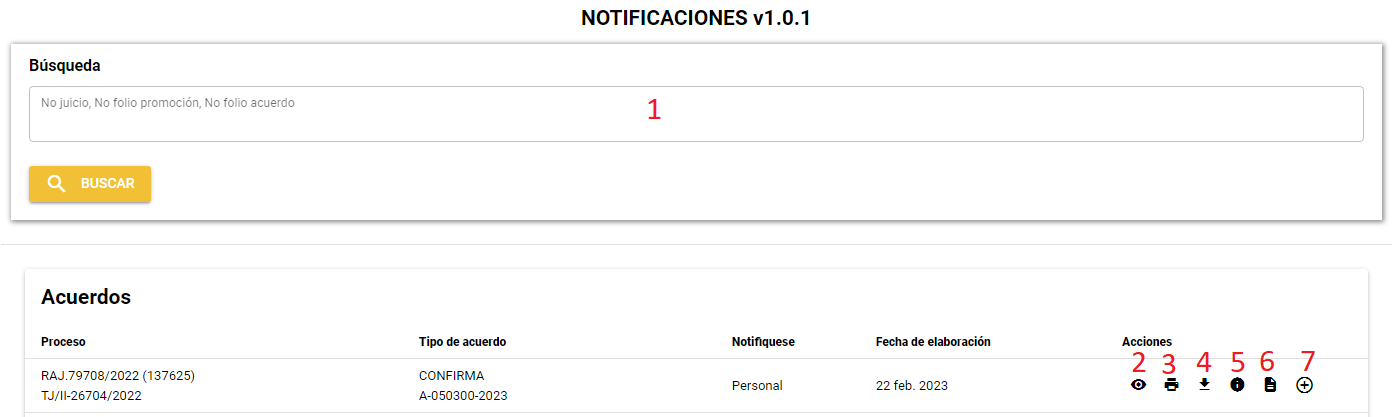
\includegraphics[width=0.88\columnwidth]{notificaciones.png}
\end{center}
\begin{enumerate}
    \item Búsqueda y consulta
    \item Visualización de documento
    \item Impresión
    \item Descarga
    \item Información del acuerdo
    \item Notificaciones
    \item Registrar notificación
\end{enumerate}
\newpage
{\Huge{\color{myblue} \section{ ¿Cómo buscar una notificación?}\label{sec:0.1}}}

 Para consultar una notificación debes ingresar número de juicio, folio o R.A en el campo de búsqueda indicado anteriormente con el número (1) y dar click en el botón {\bf{<<Buscar>>}}\\

Se mostrarán los resultados de la búsqueda.

\begin{center}
    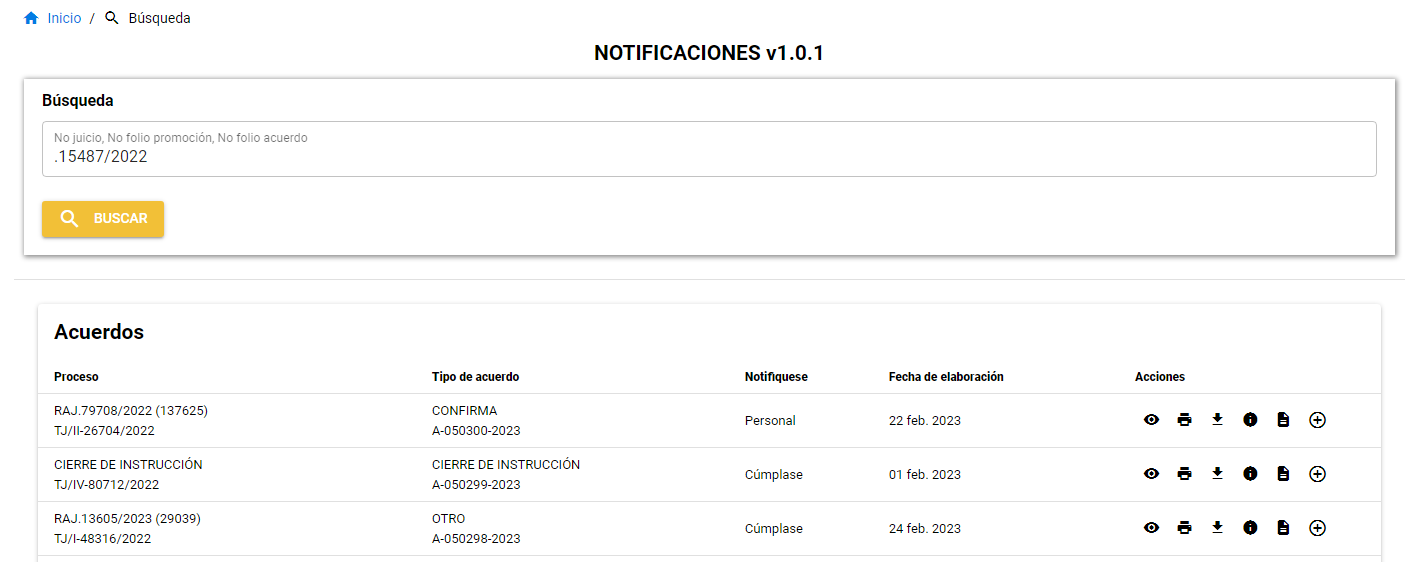
\includegraphics[width=0.88\columnwidth]{resultados_mot.png}
\end{center}

{\Huge{\color{myblue} \section{ ¿Cómo visualizar el archivo del acuerdo?}\label{sec:0.2}}}

Es necesario que previamente se haya realizado la búsqueda de  la notificación deseada \textit{Ver ~\nameref{sec:0.1}}\\
Da click sobre el icono de {\bf{<<Visualizar>>}} indicado anteriormente con el número (2), automáticamente se mostrará el archivo.

\begin{center}
    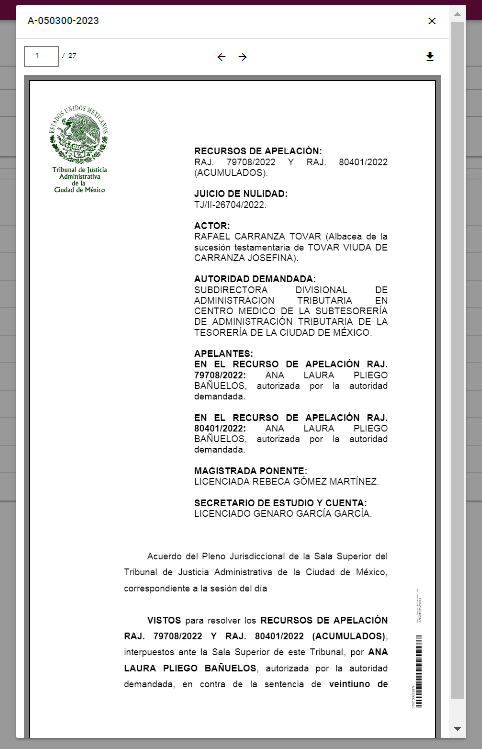
\includegraphics[width=0.21\columnwidth]{archivo.png}
\end{center}

{\Huge{\color{myblue} \section{ ¿Cómo imprimir un acuerdo?}\label{sec:0.3}}}

Es necesario que previamente se haya realizado la búsqueda de  la notificación deseada \textit{Ver ~\nameref{sec:0.1}}\\
Da click sobre el icono de {\bf{<<Imprimir>>}} indicado anteriormente con el número (3), se mostrará la pantalla con las opciones de impresión:

\begin{center}
    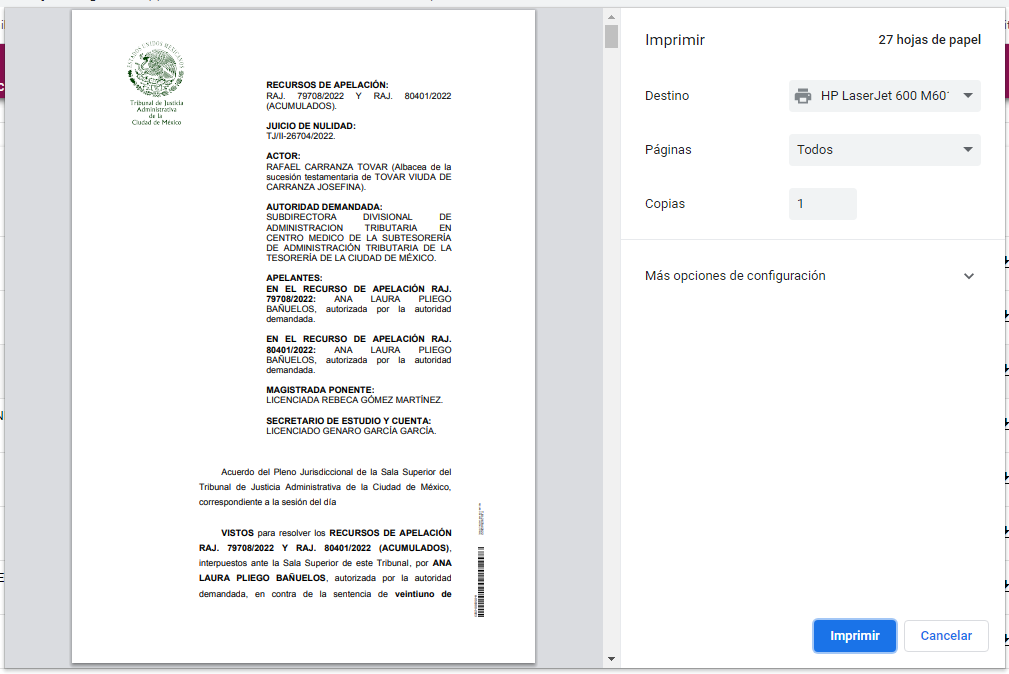
\includegraphics[width=0.66\columnwidth]{imprimir_not.png}
\end{center}

Da click en el botón {\bf{<<Imprimir>>}}.

{\Huge{\color{myblue} \section{ ¿Cómo descargar un acuerdo?}\label{sec:0.4}}}

Es necesario que previamente se haya realizado la búsqueda de  la notificación deseada \textit{Ver ~\nameref{sec:0.1}}\\
Da click sobre el icono de {\bf{<<Descargar>>}} indicado anteriormente con el número (4), automáticamente se iniciará la descarga en tu equipo de computo.

\begin{center}
    
\includegraphics[width=0.88\columnwidth]{guardar.png}
\end{center}

{\Huge{\color{myblue} \section{ ¿Cómo consultar la información del acuerdo?}\label{sec:0.55}}}

Es necesario que previamente se haya realizado la búsqueda de  la notificación deseada \textit{Ver ~\nameref{sec:0.1}}\\
Da click sobre el icono de {\bf{<<Información>>}} indicado anteriormente con el número (5), se mostrará una pantalla con la información del acuerdo.

\begin{center}
    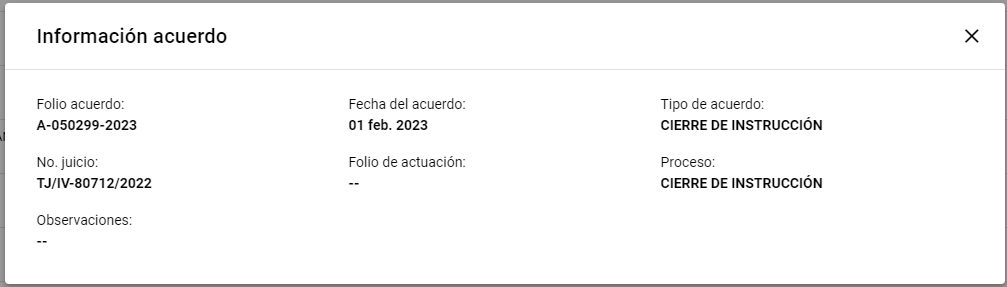
\includegraphics[width=0.88\columnwidth]{inf_acuerdo.png}
\end{center}

\begin{itemize}
    \item Folio acuerdo
    \item No.juicio
    \item Observaciones
    \item Fecha de acuerdo
    \item Folio de actuación
    \item Tipo de acuerdo
\end{itemize}

{\Huge{\color{myblue} \section{ ¿Cómo ver las notificaciones del acuerdo?}\label{sec:0.5}}}

Es necesario que previamente se haya realizado la búsqueda de  la notificación deseada \textit{Ver ~\nameref{sec:0.1}}\\
Da click sobre el icono de {\bf{<<Notificaciones>>}} indicado anteriormente con el número (6), se desplegarán la información de las notificaciones.

\begin{center}
    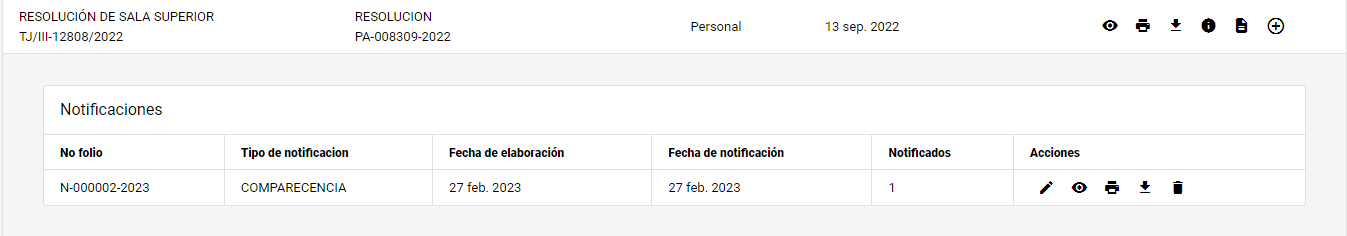
\includegraphics[width=0.88\columnwidth]{noti.png}
\end{center}

Podemos editar, visualizar, imprimir, descargar y eliminar la notificación con los iconos de acciones.

{\Huge{\color{myblue} \section{ ¿Cómo registrar una notificación?}\label{sec:0.6}}}

Es necesario que previamente se haya realizado la búsqueda de  la notificación deseada \textit{Ver ~\nameref{sec:0.1}}\\
Da click sobre el icono de {\bf{<<Notificaciones>>}} indicado anteriormente con el número (7), se mostrará la siguiente pantalla:

\begin{center}
    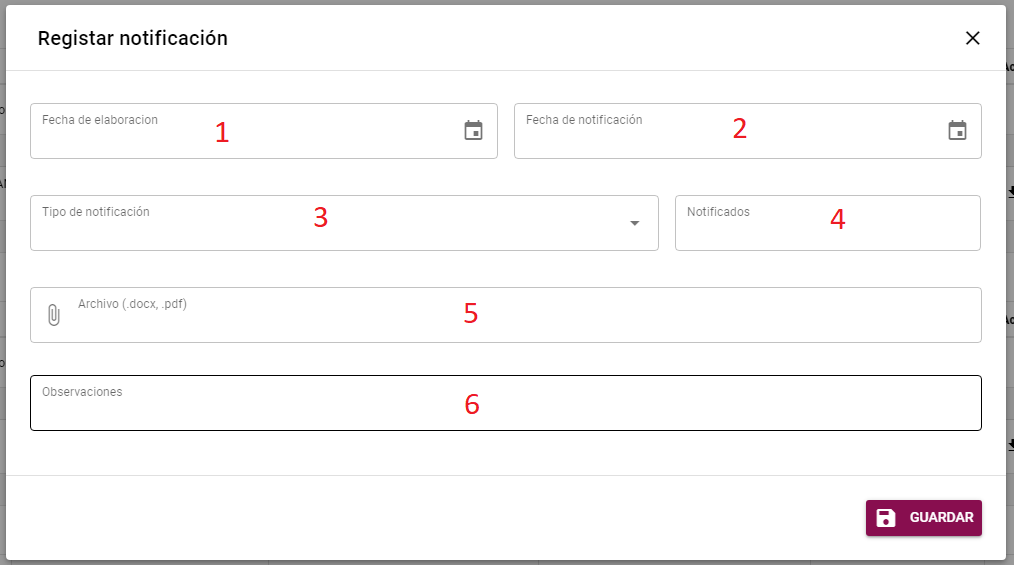
\includegraphics[width=0.88\columnwidth]{reg_noti.png}
\end{center}

Ingresa los siguientes datos:

\begin{enumerate}
    \item Fecha de elaboración
    \item Fecha de notificación
    \item Tipo de notificación
    \item Notificados
    \item Archivo (.docx .pdf)
    \item Observaciones
\end{enumerate}

Da click en el botón {\bf{<<Guardar>>}}, se mostrará el siguiente mensaje:
\begin{center}
    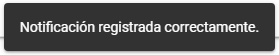
\includegraphics[width=0.30\columnwidth]{notiguardada.png}
\end{center}

\chapter{\large{Estrados y boletín electrónico.}}\label{chap:boletin}

En el módulo de {\bf Listado de estrados y boletín electrónico} podrá realizar las siguientes actividades:

\begin{itemize}
    \item Registro de listados.
    \item Escaneo de acuerdos.
    \item Consultar listados.
    \item Editar listados.
    \item Impresión de listados.
    \item Exportar listados.
\end{itemize}

{\bf{Datos del módulo consulta}}

\begin{enumerate}[(1)]
    \item Sección de búsqueda.
    \item Sección de listados de acuerdos
    \item Iconos 
    \begin{itemize}
    	\item Imprimir
	    \item Exportar
    	\item Consultar
	    \item Eliminar listado
	\end{itemize}
\end{enumerate}

\begin{center}
    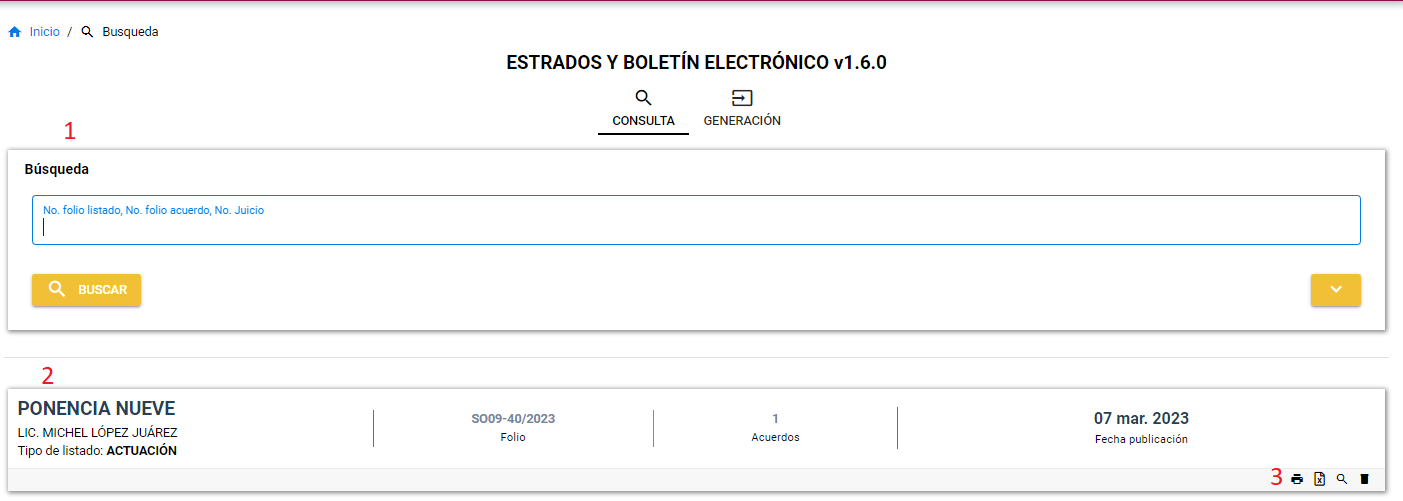
\includegraphics[width=0.88\columnwidth]{datos_consulta.png}
\end{center}


{\Huge{\color{myblue} \section{ ¿Cómo registrar un listado de acuerdos?}\label{sec:6}}}

\begin{center}
    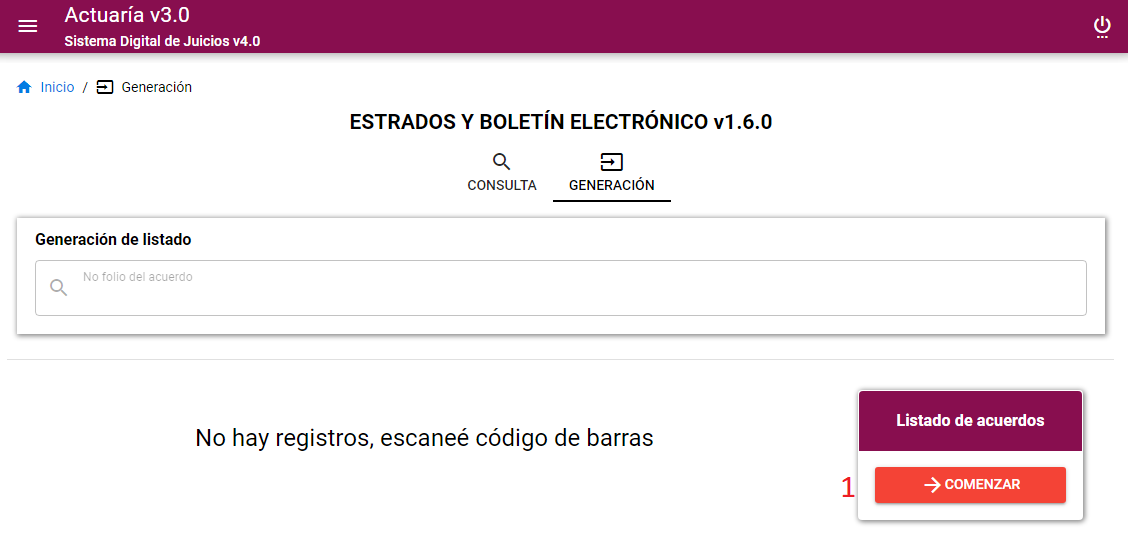
\includegraphics[width=0.88\columnwidth]{boletin.png}
\end{center}

1. Para generar un listado de acuerdos deberá dar click en el botón {\bf «COMENZAR»} el cual presentará la
siguiente pantalla:

\begin{center}
    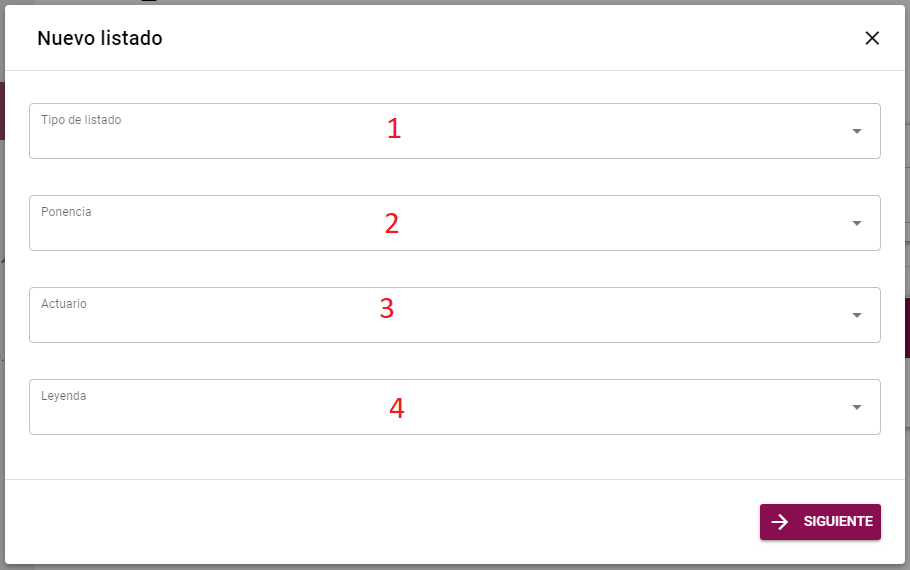
\includegraphics[width=0.66\columnwidth]{nuevo_list.png}
\end{center}

Tendrá que seleccionar las siguientes opciones:\\

\begin{enumerate}[1.]
    \item Tipo de listado
    \item Ponencia.
    \item Actuario
    \item Leyenda
\end{enumerate}

Después de llenar los 4 campos antes mencionados da click en el botón {\bf «SIGUIENTE»} donde presentará la
siguiente pantalla:

\begin{center}
    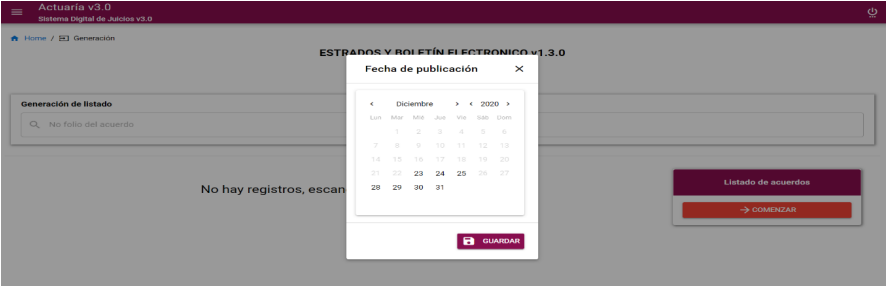
\includegraphics[width=0.88\columnwidth]{C16.png}
\end{center}

Seleccione la fecha de publicación de listado y da click en el botón {\bf «GUARDAR»}, mostrará la siguiente
pantalla:

\begin{center}
    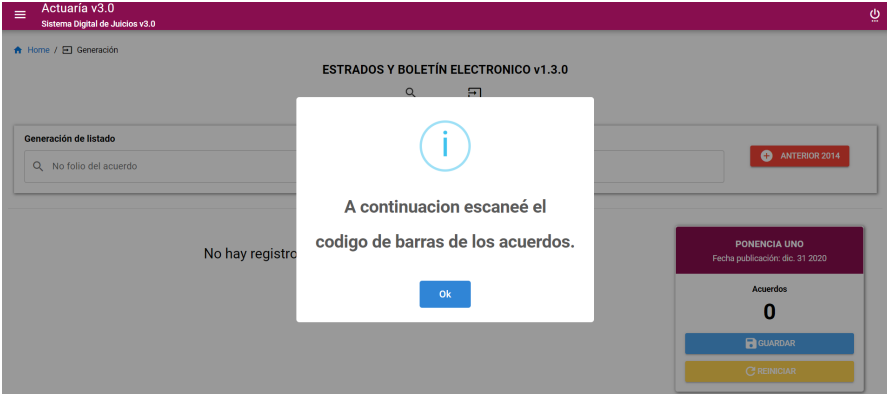
\includegraphics[width=0.88\columnwidth]{C17.png}
\end{center}

da click en {\bf «OK»}, o espera 3 segundos y se quitara automáticamente.

{\Huge{\color{myblue} \section{ ¿Cómo escaneo el código de barras de los acuerdos?}\label{sec:7}}}

Para ingresar acuerdos en el listado, se podrá escanear el folio que se encuentra en la parte inferior del
acuerdo generado por el sistema digital de juicios.

\begin{center}
    
\includegraphics[width=0.30\columnwidth]{C18.png}
\end{center}

En el contenedor mostrará el listado de los acuerdos con la siguiente información:

\begin{itemize}
    \item Actor.
    \item Promoción.
    \item Número de juicio.
    \item Folio del acuerdo.
    \item Tipo de acuerdo.
\end{itemize}

\begin{center}
    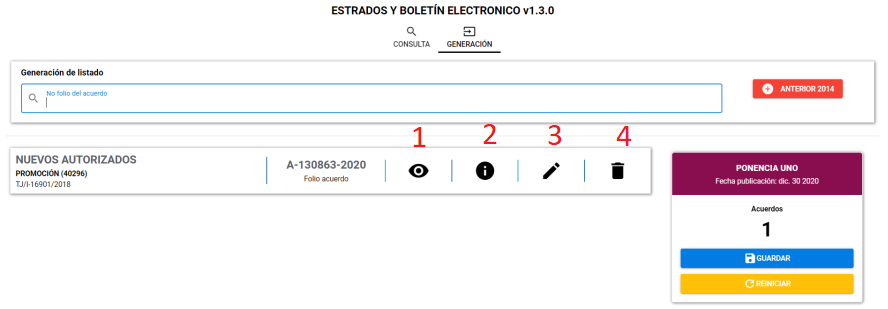
\includegraphics[width=0.88\columnwidth]{C19.png}
\end{center}

\begin{itemize}
    \item Podrá visualizar el acuerdo dando click en el icono con el {\bf número {1}}.
    \item Podrá visualizar la información dando click en el icono con el {\bf número {2}}
    \item Podrá editar la observaciones dando click en el icono con el {\bf número {3}}.
    \item Podrá eliminar un acuerdo dando click en el icono con el {\bf número {4}}.
    \item Podrá reiniciar el listado dando click en el botón {\bf «REINICIAR»}.
\end{itemize}

Para terminar el registro de la lista deberá dar click en el botón {\bf «GUARDAR»}, el sistema mostrara un mensaje de
confirmación y redireccionara al listado generado.

{\Huge{\color{myblue} \section{ ¿Cómo registrar juicios anteriores al año 2014?}\label{sec:8}}}

Para registrar juicios anteriores al 2014 solo deberá dar click en el botón {\bf «ANTERIOR 2014»},

\begin{center}
    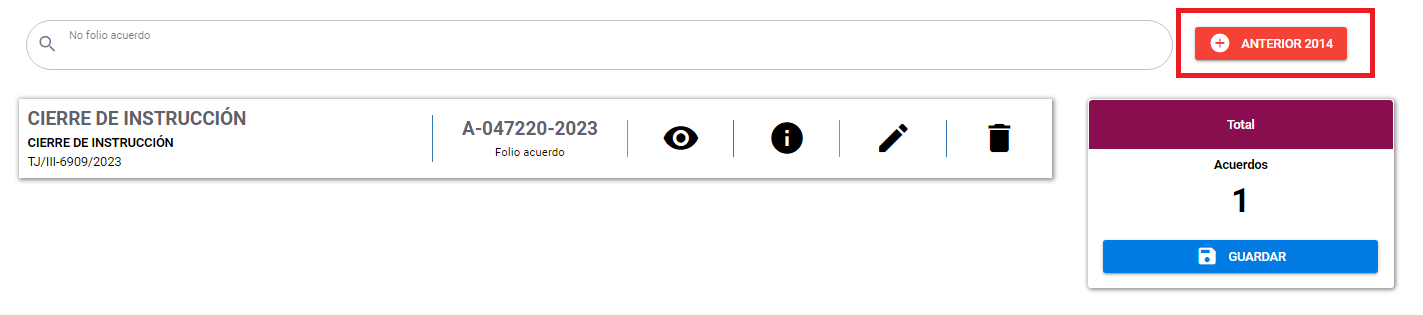
\includegraphics[width=0.88\columnwidth]{anterio2014.png}
\end{center}

Se mostrará la siguiente pantalla:

\begin{center}
    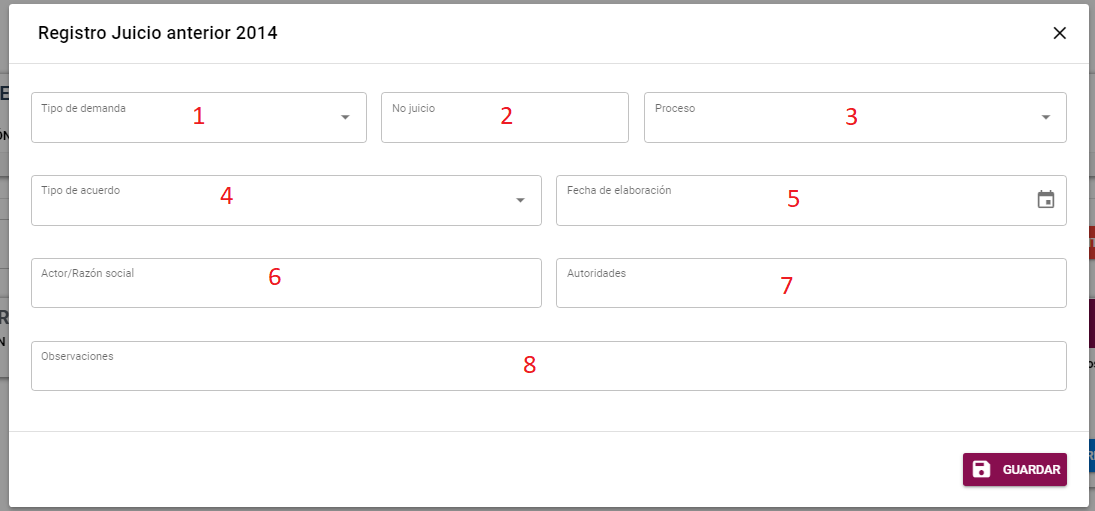
\includegraphics[width=0.88\columnwidth]{anterior2014.png}
\end{center}

Se requiere ingresar los siguientes datos ya que son campos obligatorios:

\begin{itemize}
    \item Tipo de demanda.
    \item Número de juicio.
    \item Proceso.
    \item Tipo de acuerdo.
    \item Fecha de elaboración.
    \item Actor/Razón social.
    \item Autoridades.
\end{itemize}

Las observaciones son opcionales, una vez que se ingresó toda la información, da click en el botón
{\bf «GUARDAR»}, para que lo agregue a lista que ya se tiene generada.


{\Huge{\color{myblue} \section{ ¿Cómo buscar un listado de estrados?}\label{sec:9}}}

\begin{center}
    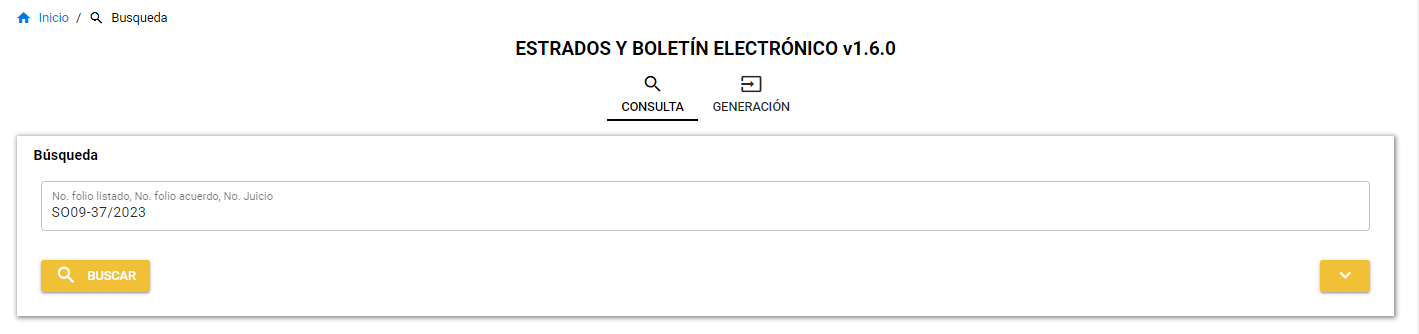
\includegraphics[width=0.88\columnwidth]{busqueda_bol.png}
\end{center}

Para poder realizar la búsqueda es necesario tener al menos uno de los siguientes datos que se
enlistan:

\begin{itemize}
    \item Número de listado.
    \item Número de folio del acuerdo.
\end{itemize}

Después de ingresar uno de los dos datos mencionados anteriormente debe dar click el botón
{\bf «BUSCAR»}, para que muestre los resultados obtenidos.\\

Para obtener una búsqueda más avanzada y precisa de click en el botón con el {\bf {número 1}} y se mostrará la siguiente pantalla.

\begin{center}
    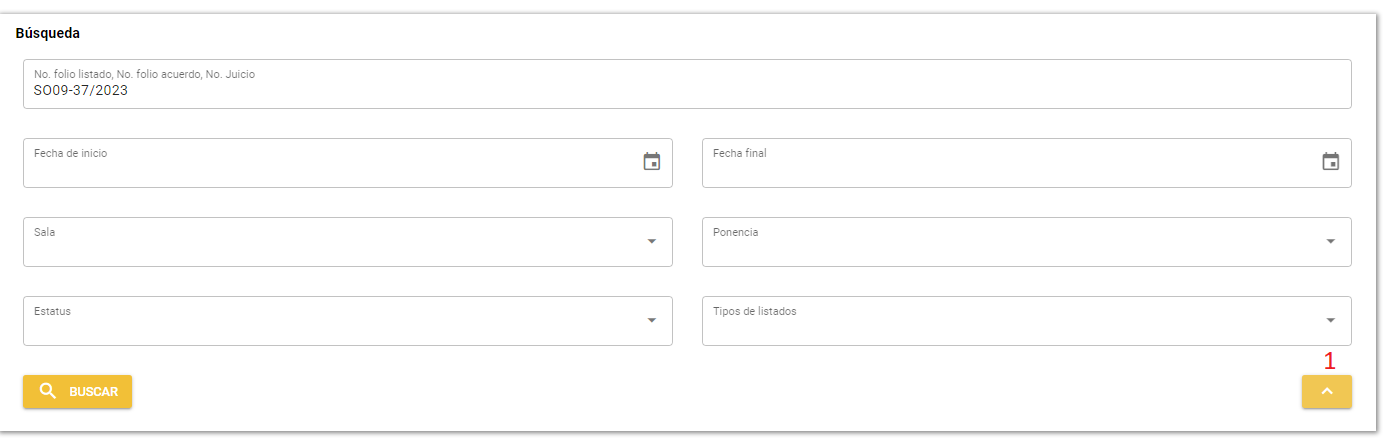
\includegraphics[width=0.88\columnwidth]{busqueda_avan.png}
\end{center}

La cual muestra los siguientes datos:

\begin{itemize}
    \item Número de listado, No. de folio acuerdo, No Juicio
    \item Fecha inicio.
    \item Fecha final.
    \item Sala.
    \item Ponencia.
    \item Estatus
    \item Tipo de listado
\end{itemize}

Ingresados los datos para la búsqueda solo debe de dar click el botón de {\bf «BUSCAR»}, para que realice
la búsqueda y muestre los resultados obtenidos por el sistema.

{\Huge{\color{myblue} \section{ ¿Cómo editar un listado de estrados?}\label{sec:10}}}

Para poder editar un listado de estrados es necesario realizar la búsqueda de la lista como se describe anteriormente.

Una vez realizada la búsqueda mostrara la siguiente pantalla con los resultados obtenidos:

\begin{center}
    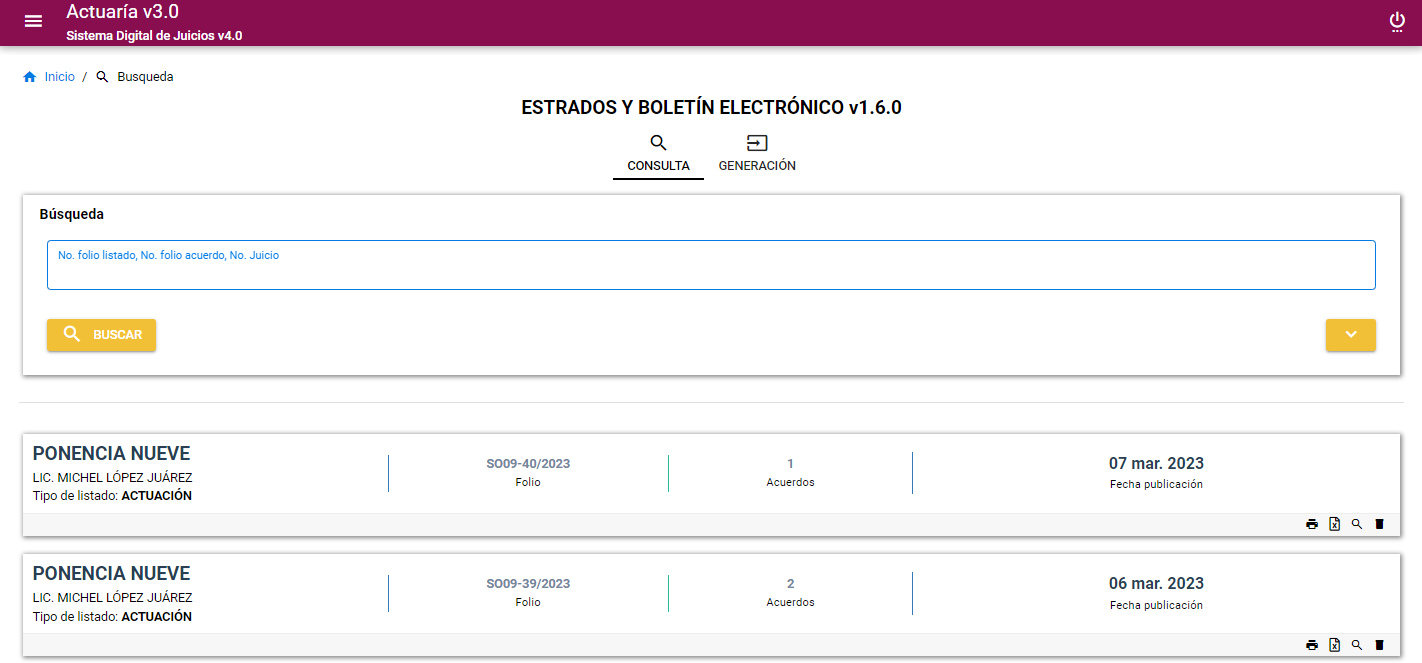
\includegraphics[width=0.88\columnwidth]{busqueda_list.png}
\end{center}

Da click en icono de {\bf {<<Consultar>>}} que tiene forma de lupa.\\
Se mostrará una pantalla similar.

\begin{center}
    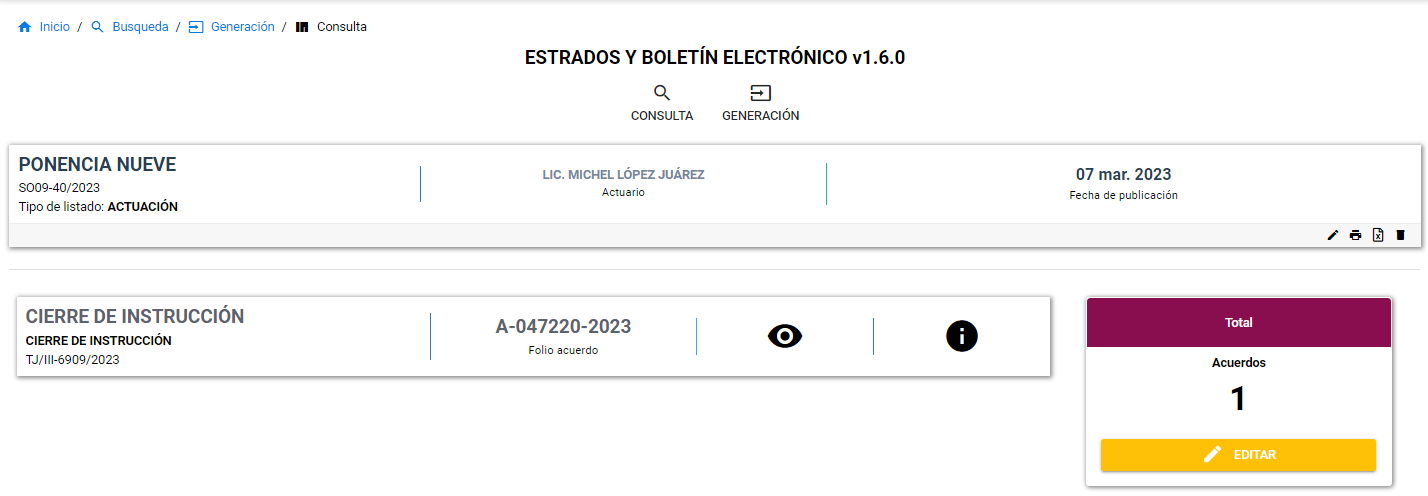
\includegraphics[width=0.88\columnwidth]{editar_list.png}
\end{center}

Ahí se presenta los datos del listado, con el número total de acuerdos que contiene la lista y los
datos de cada uno de los acuerdos. Para poder editar el listado deberá dar click en el botón {\bf «EDITAR»},
para que presente las siguientes pantallas:

\begin{center}
    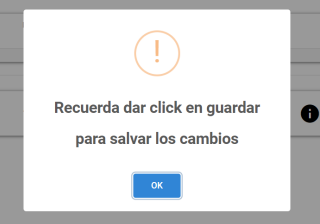
\includegraphics[width=0.44\columnwidth]{C27.png}
\end{center}

Muestra un mensaje de recordatorio para guardar los cambios realizados. Después presentara la siguiente pantalla:

\begin{center}
    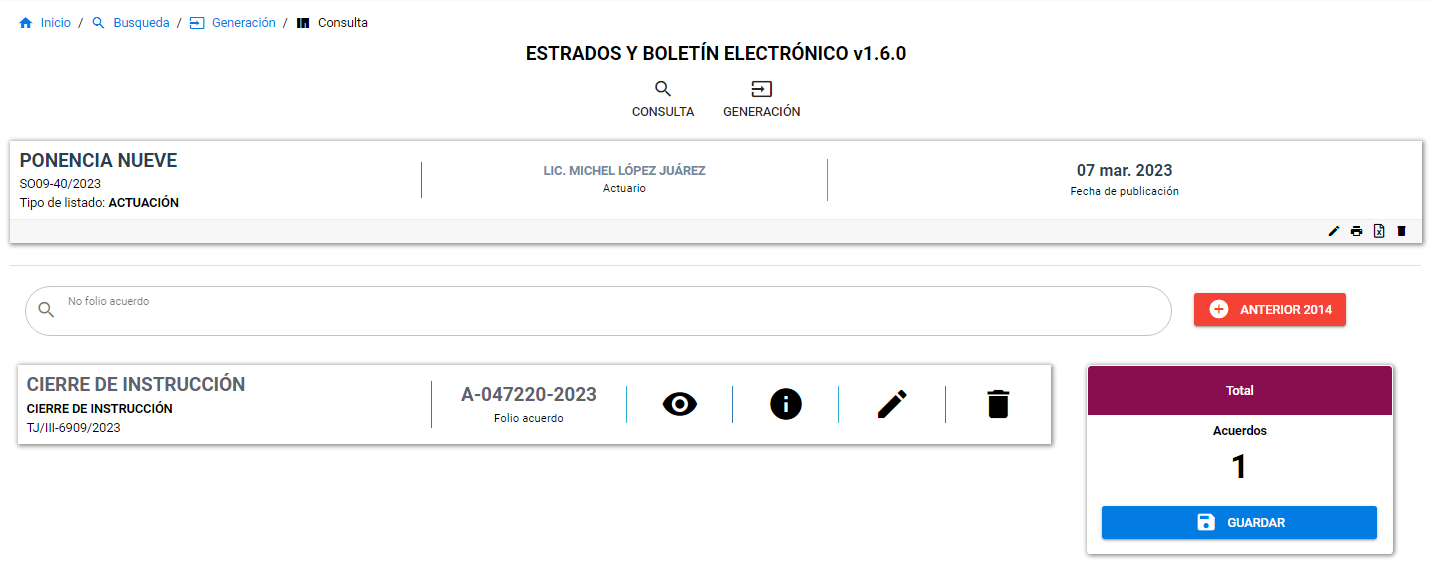
\includegraphics[width=0.88\columnwidth]{editar_list2.png}
\end{center}

Donde se ingresarán o escanearan los acuerdos
\textit{Ver ~\nameref{sec:6}}

{\bf NOTA: Recuerda dar click el botón «GUARDAR», para que los cambios realizados se guarden.} 

{\color{myblue}\section{\normalfont\sffamily{ ¿Cómo se modifican los datos del listado (Ponencia, Actuario, Fecha de publicación y leyenda)?}}}\label{sec:11}

Para modificar la información del listado es necesario consultar el listado \textit{Ver ~\nameref{sec:9}} y dar click en el icono {\bf{<<Editar>>}} como
se muestra a continuación:

\begin{center}
    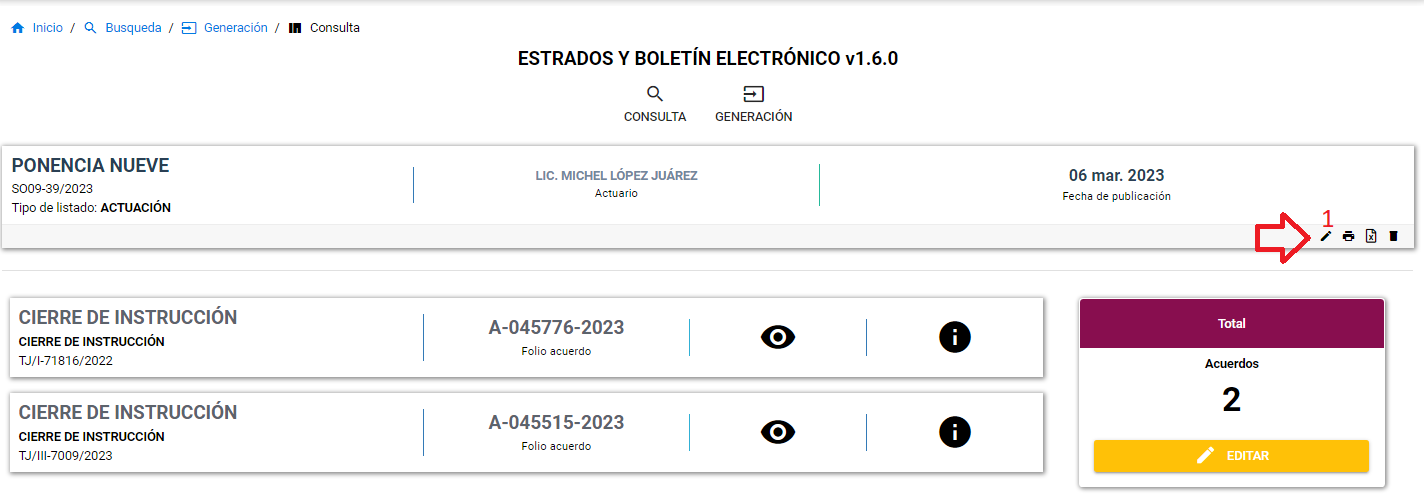
\includegraphics[width=0.88\columnwidth]{editar_acuer.png}
\end{center}

\vspace{2cm}
Se mostrará la pantalla siguiente donde podrá editar los datos deseados.

\begin{center}
    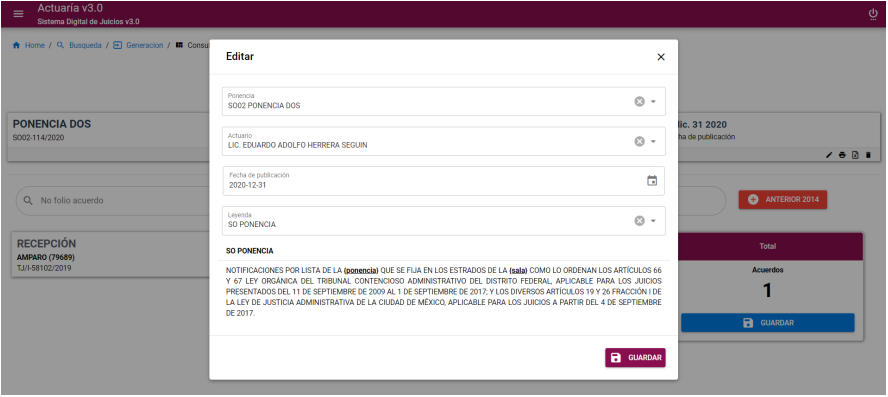
\includegraphics[width=0.88\columnwidth]{C30.png}
\end{center}

Una vez modificada la información, dar click el botón {\bf «GUARDAR»} para que los cambios realizados se guarden correctamente. 

{\color{myblue}\section{\normalfont\sffamily{ ¿Cómo imprimir un listado?}}}\label{sec:11.1}

Hay dos maneras de imprimir un listado la primera es desde el módulo consulta dando click en el icono {\bf {<<Imprimir>>}}

\begin{center}
    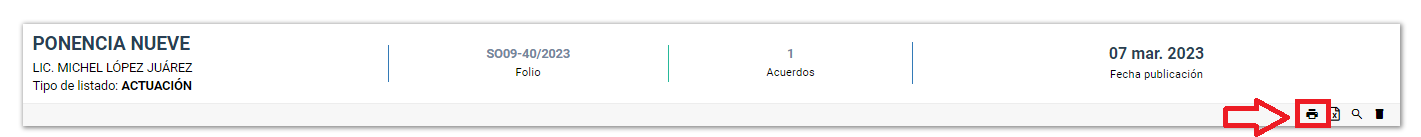
\includegraphics[width=0.88\columnwidth]{imprimir.png}
\end{center}

Se abrirá una ventana con el documento listo para imprimir

\begin{center}
    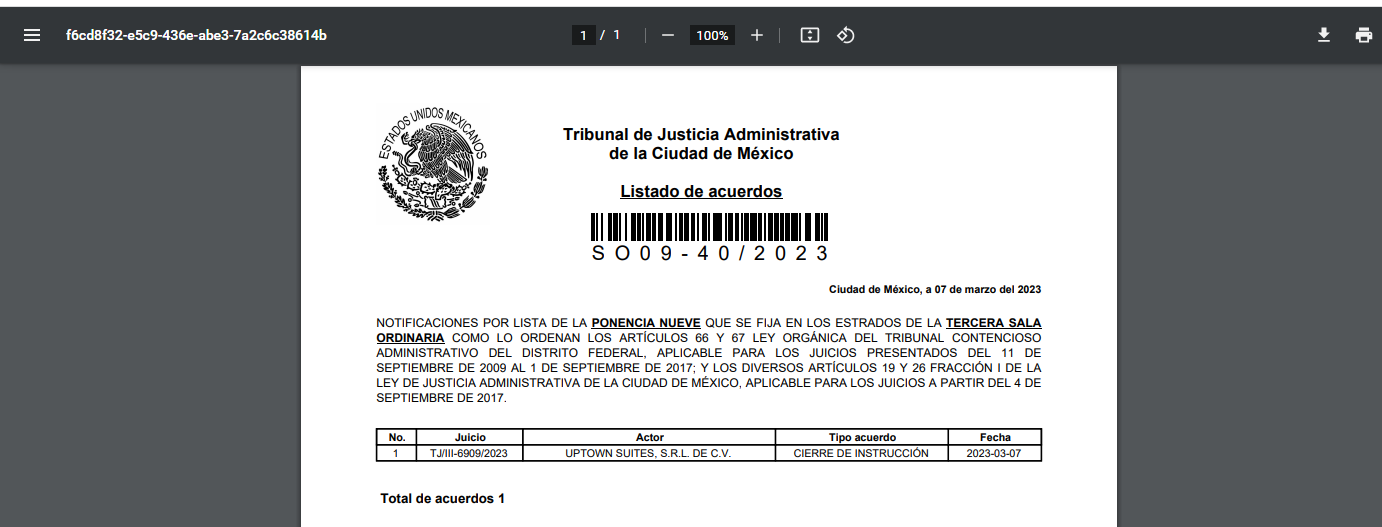
\includegraphics[width=0.66\columnwidth]{imprimir1.png}
\end{center}

\chapter{\large{Sistema de Citas para Oficialía y Actuaría de Sala Superior (SCO).}}\label{}

En el Sistema de Citas para la Oficialía y Actuaría de Sala Superior, podrá realizar las siguientes actividades:

\begin{itemize}
    \item Buscar cita SCO.
    \item Información cita.
    \item Imprimir acuses.
    \item Descargar acuses.
    \item Cancelar cita.
    \item Reporte PDF.
    \item Reporte EXCEL.
\end{itemize}

\vspace{2cm}
Para poder realizar la búsqueda es necesario contar con al menos uno de los siguientes datos:

\begin{itemize}
    \item Número de folio de cita.
    \item Fecha de cita.
\end{itemize}

\begin{center}
    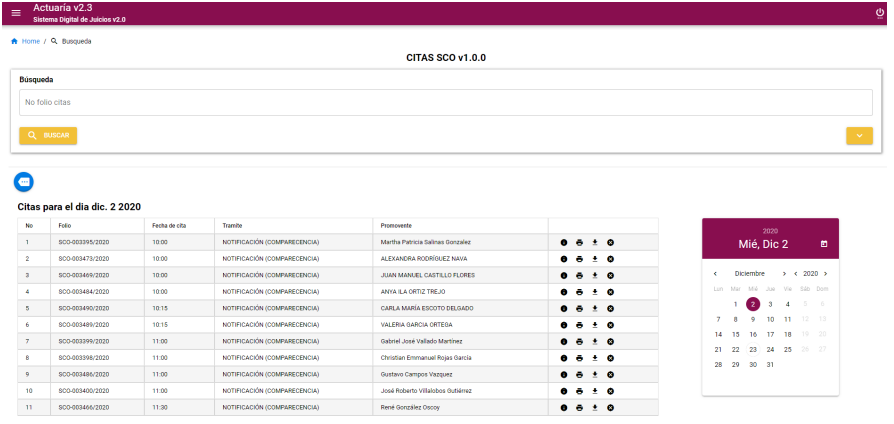
\includegraphics[width=0.88\columnwidth]{C50.png}
\end{center}

Para obtener una búsqueda más avanzada y precisa de click en el botón identificado con el {\bf{número 1}} y se mostrará la siguiente pantalla:

\begin{center}
    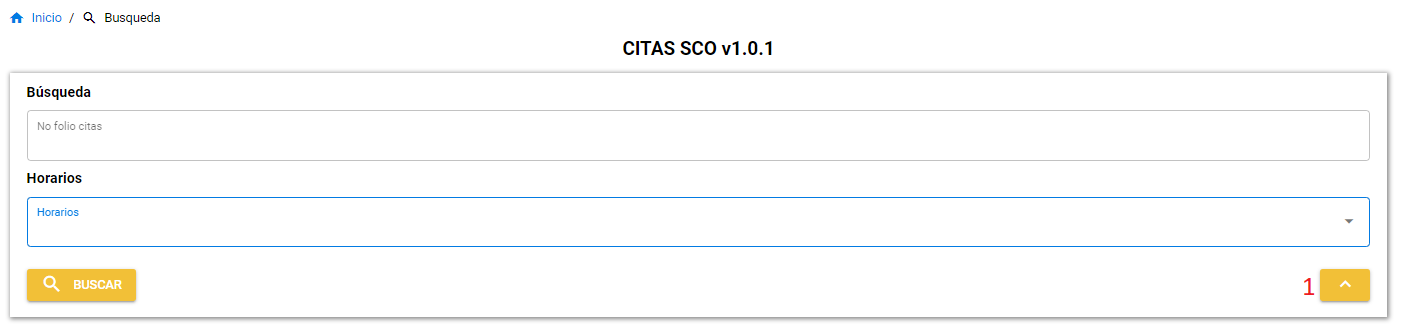
\includegraphics[width=0.88\columnwidth]{citas.png}
\end{center}

La cual contiene el campo para seleccionar los tipos de horarios

Seleccionado el tipo de horario da click el botón de {\bf «BUSCAR»}, para que realice la búsqueda y
muestre los resultados obtenidos por el sistema.\\

\vspace{1cm}

{\bf {Descripción de las acciones de cada icono:}}

1. Información cita.

\begin{center}
    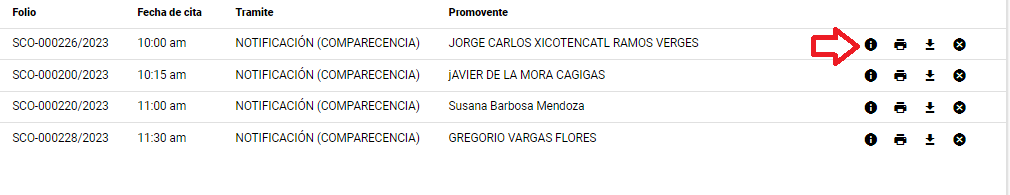
\includegraphics[width=0.88\columnwidth]{citassci.png}
\end{center}


Para visualizar la información de la cita da click en el icono de ''información'' y se mostrara una pantalla similar.

\begin{center}
    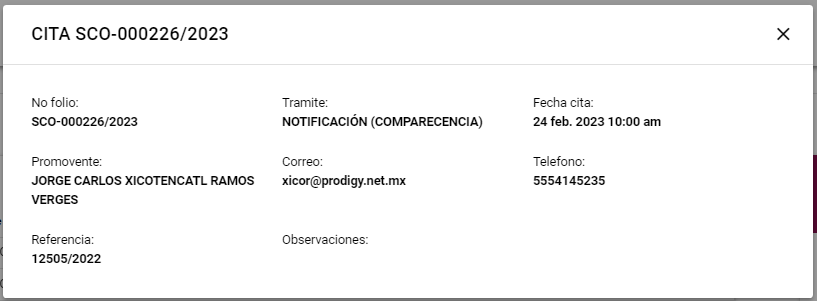
\includegraphics[width=0.75\columnwidth]{inf.png}
\end{center}

2. Imprimir acuses

Para imprimir un acuse da click sobre el icono ''Imprimir''

\begin{center}
    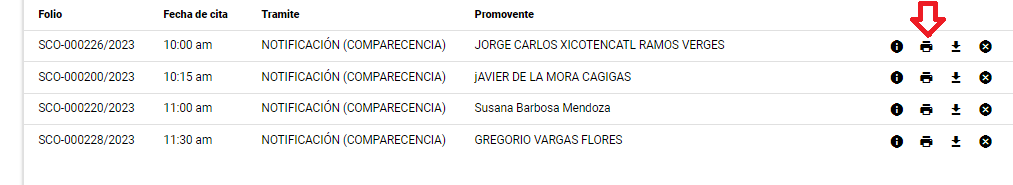
\includegraphics[width=0.75\columnwidth]{imprimiracuse.png}
\end{center}

Se mostrará la ventana de impresión, dar click en el botón {\bf «Imprimir»}.
\begin{center}
    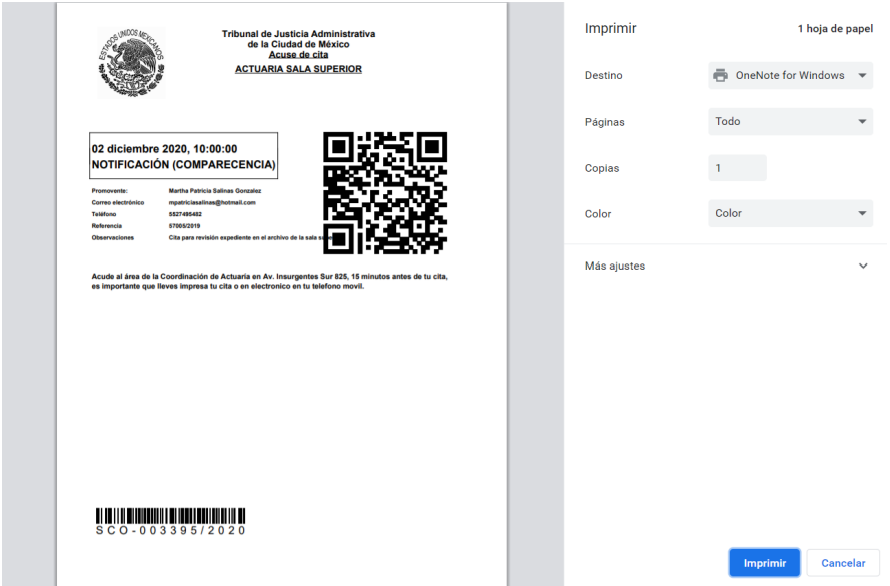
\includegraphics[width=0.8\columnwidth]{C54.png}
\end{center}

\newpage
3.Descargar acuses\\
La descarga de acuses de la cita se realiza dando click en el icono ''Descargar'' 
\begin{center}
    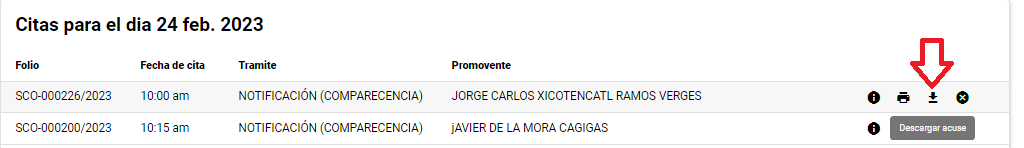
\includegraphics[width=0.88\columnwidth]{descargar_A.png}
\end{center}
El archivo se descargará en su equipo.

\vspace{1cm}

4. Reportes de citas

Para poder generar reporte de citas da click en el icono señalado, mostrara que tipo de reporte.

\begin{itemize}
    \item Reporte PDF.
    \item Reporte EXCEL.
\end{itemize}

\begin{center}
    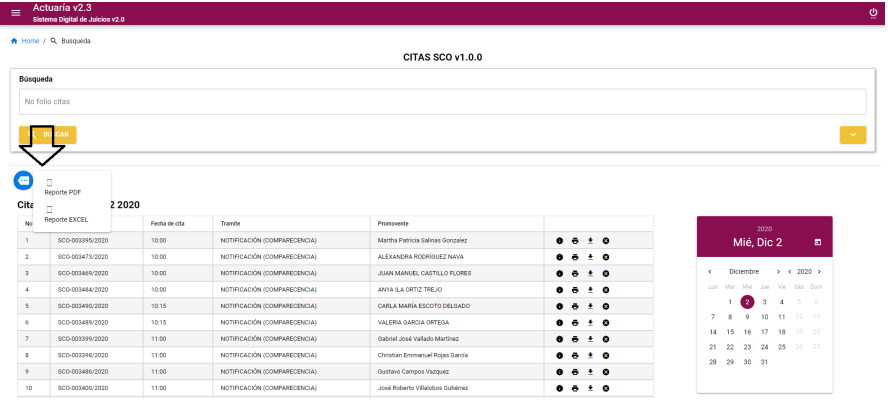
\includegraphics[width=0.88\columnwidth]{C56.png}
\end{center}

Al seleccionar el tipo de reporte, la descarga comenzara automáticamente, lo mostrara en la barra
de descargas.

\begin{center}
    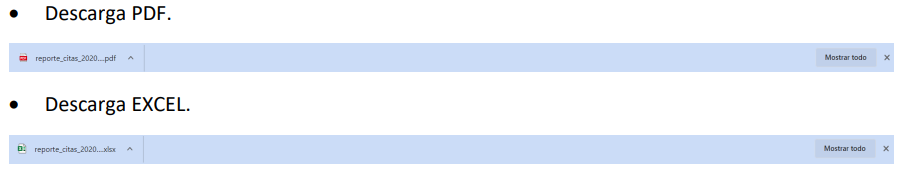
\includegraphics[width=0.88\columnwidth]{C57.png}
\end{center}

\chapter{\large{Generación de cédulas v2.0.0}}\label{chap:cedulas}
{\Huge{\color{myblue} \section{¿Cómo generar una cédula?}\label{sec:12}}}

Daremos click en la opción {\bf{ <<Generación de cédulas v2.0.0>>  }}

\begin{center}
    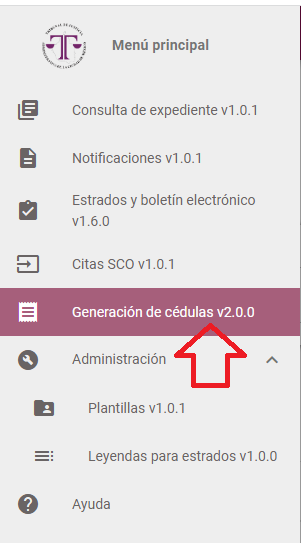
\includegraphics[width=0.20\columnwidth]{cedulas.png}
\end{center}

Para generar una cédula existe 3 opciones:

 \begin{enumerate}[(1)] 
        \item Escaneando el folio del acuerdo.
	\item Ingresando el folio manualmente.
	\item Subiendo archivo de excel con los folios de acuerdo.
\end{enumerate}


\begin{center}
    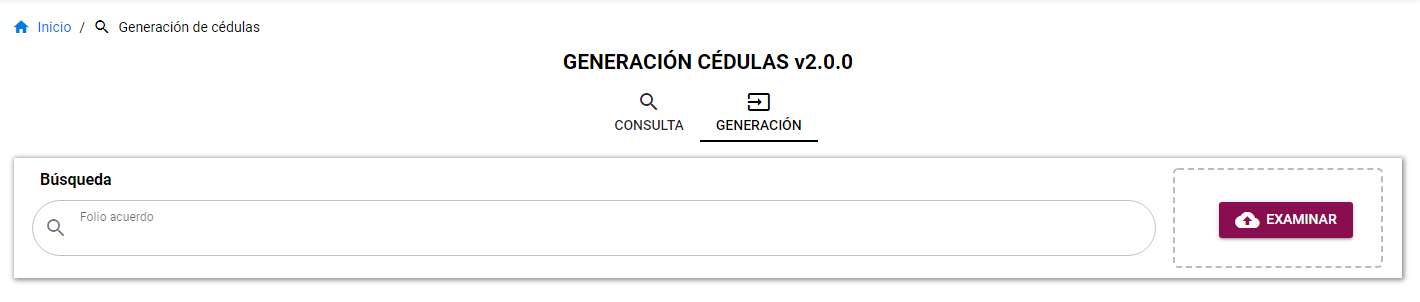
\includegraphics[width=0.90\columnwidth]{exam.png}
\end{center}

Después de escanear o ingresar manualmente el folio nos mostrara la siguiente pantalla, 
para seleccionar las notificaciones para acuerdo.

\begin{center}
    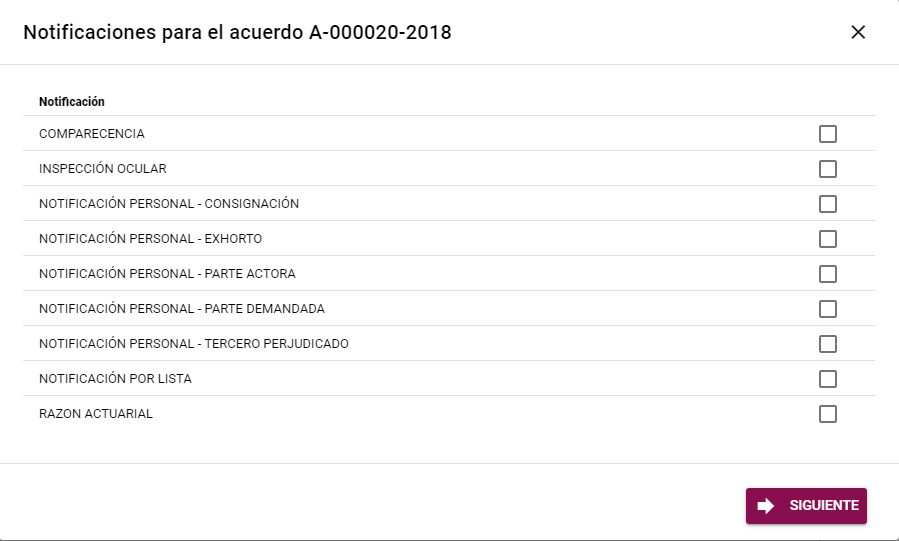
\includegraphics[width=0.90\columnwidth]{noti5.png}
\end{center}

Se podrá seleccionar más de una notificación por acuerdo. Una vez seleccionado la(s)
notificación(es), dar click en el botón {{\bf«SIGUIENTE»}}, mostrara el siguiente formulario con los siguientes
datos:

\begin{center}
    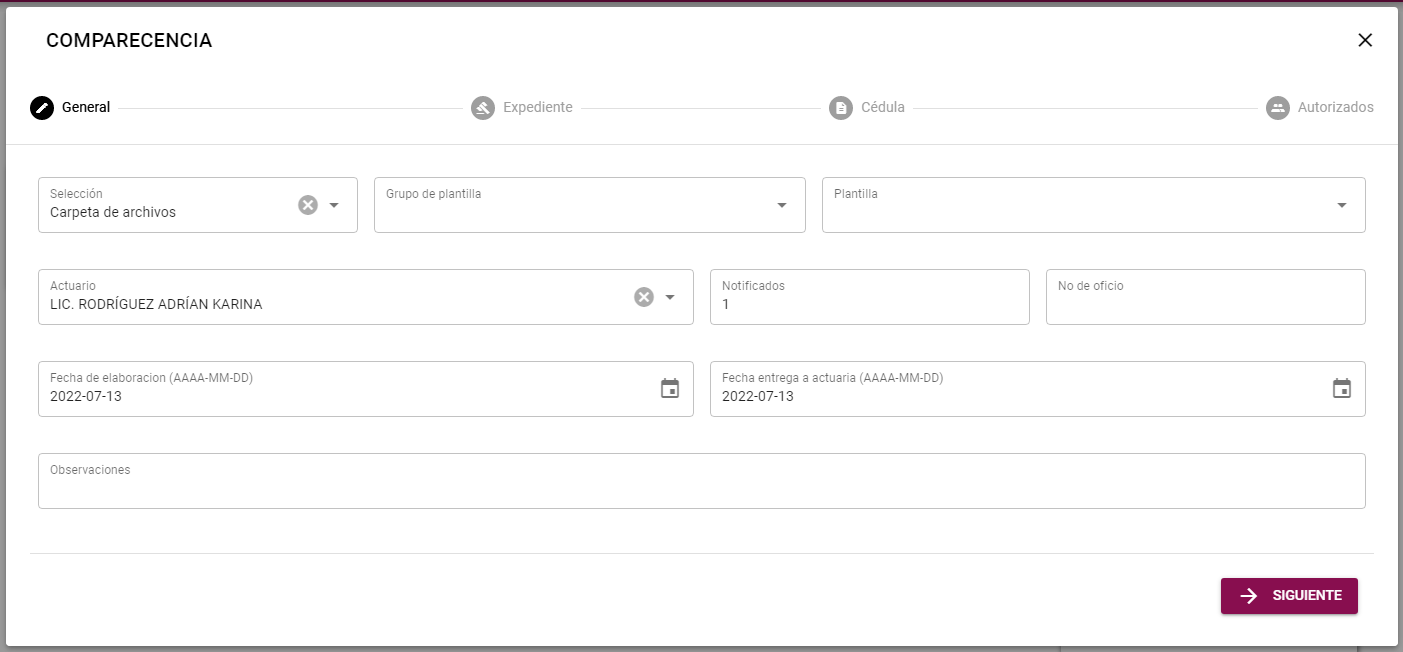
\includegraphics[width=0.90\columnwidth]{comparecencia.png}
\end{center}

\begin{itemize}
    \item Selección
    \item  Grupo de plantilla
    \item  Plantilla
    \item  Actuario
    \item  Notificados
    \item  No de oficio
    \item  Fecha entrega a actuaria
    \item  Fecha de elaboración
    \item Observaciones
\end{itemize}

En caso de no contar con una plantilla registrada en el sistema, se puede subir una plantilla
temporal.\\

Primero tienes que seleccionar:
{\bf{
<<Subir archivo>>}}y dar click en subir archivo.\\

\begin{center}
    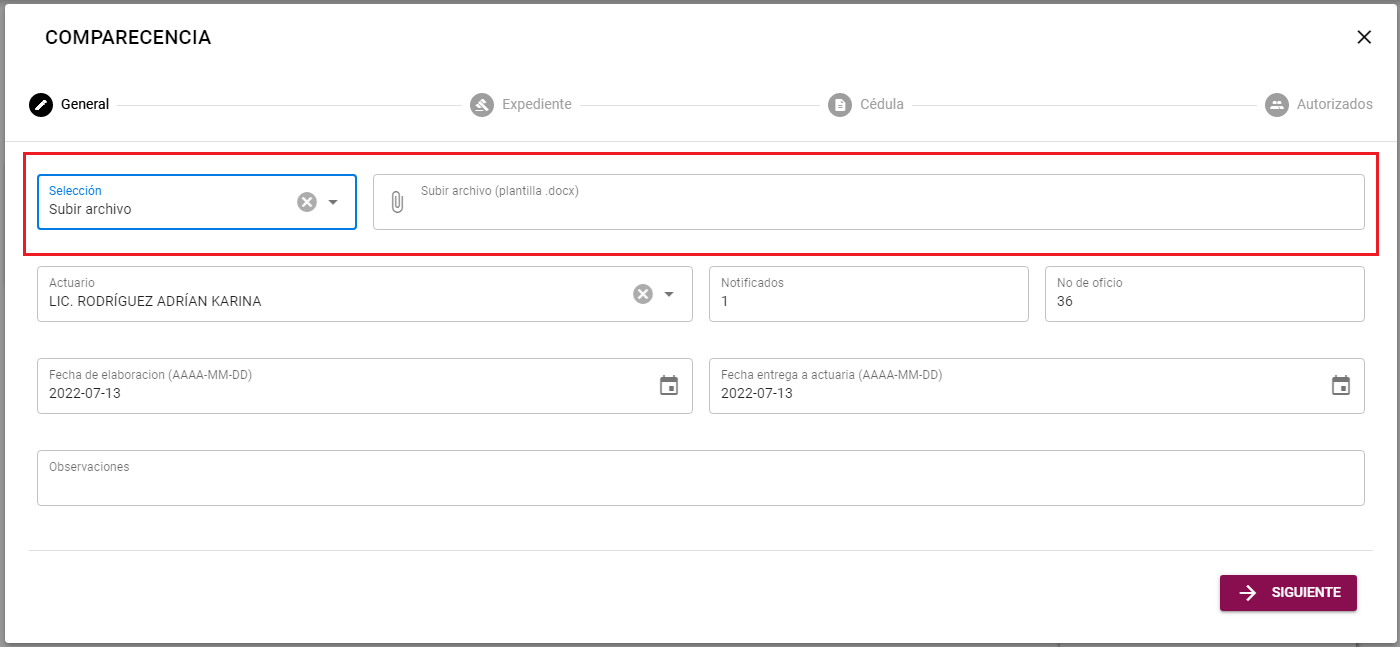
\includegraphics[width=0.90\columnwidth]{comparecencia3.png}
\end{center}

Automáticamente se abrirá una ventana donde seleccionaras tu plantilla desde tus documentos.

\begin{center}
    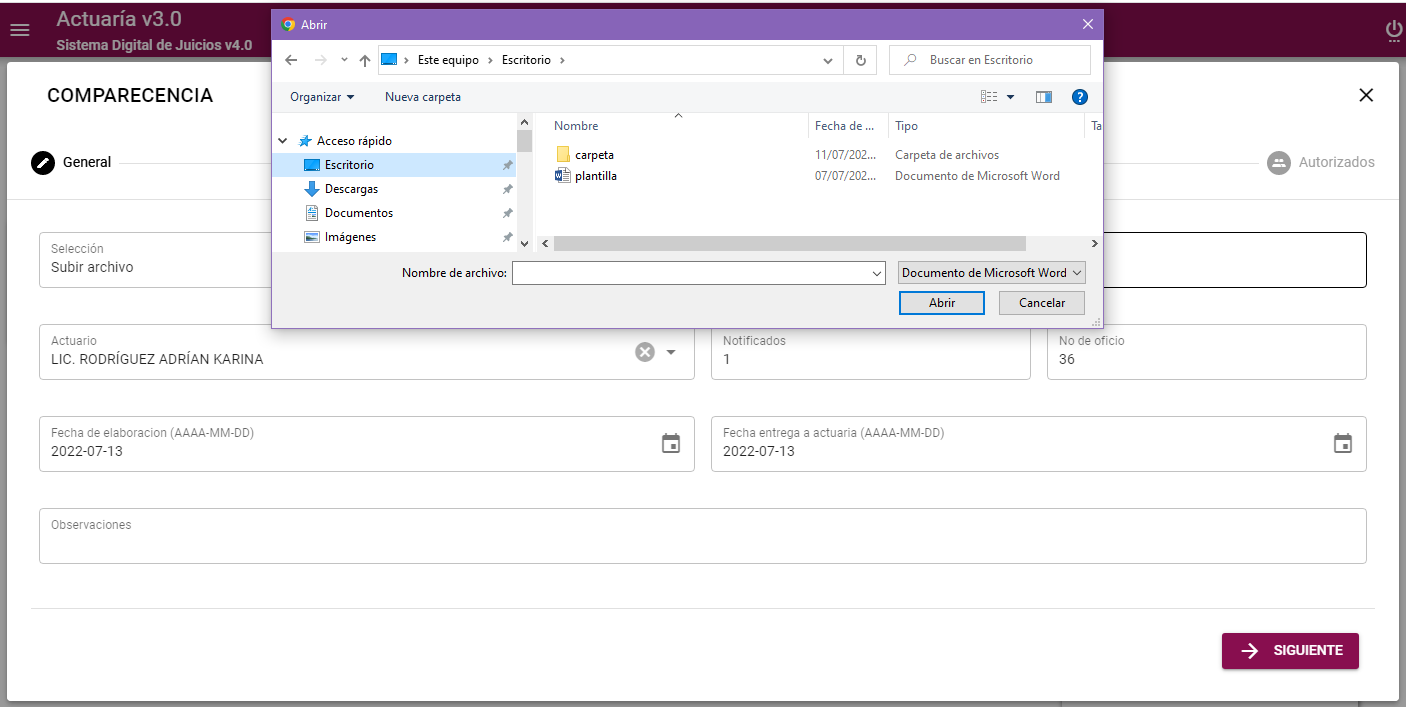
\includegraphics[width=0.90\columnwidth]{comparecencia4.png}
\end{center}

Después de ingresar los datos daremos click en el botón.
{\bf{<<SIGUIENTE>>}}
Ahora ingresaremos los siguientes datos:

 \begin{itemize}
    \item Teléfono
	\item Correo electrónico
	\item Domicilio para recibir notificaciones (*)
 \end{itemize}


\begin{center}
    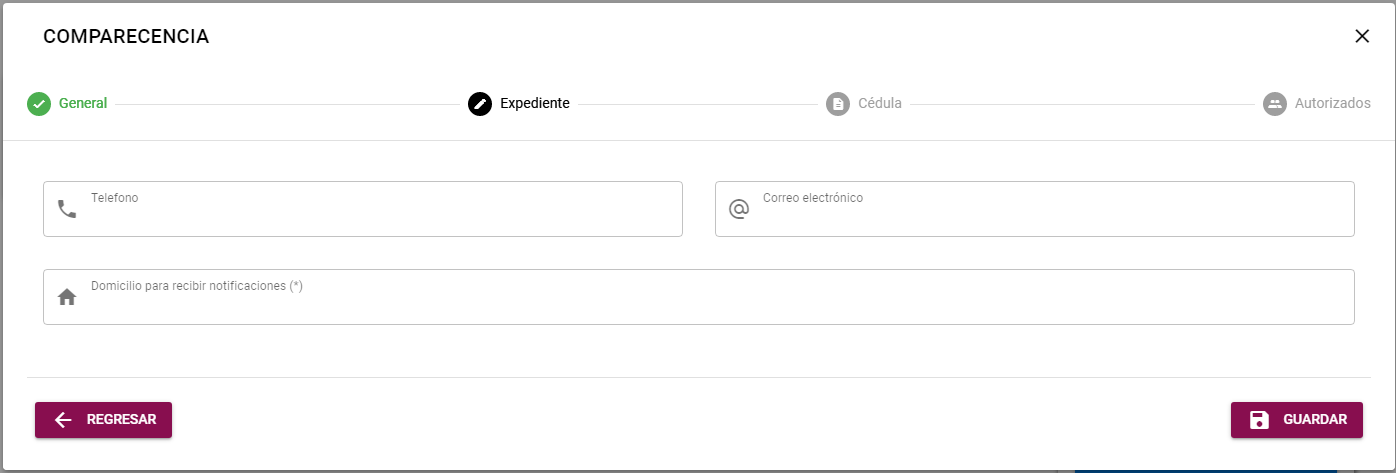
\includegraphics[width=0.90\columnwidth]{comparecencia2.png}
\end{center}

Daremos click en {\bf{
<<GUARDAR>>}}

{\Huge{\color{myblue} \section{¿Cómo generar cédula desde un archivo de Excel?}\label{sec:13}}}

Para usar la opción de  Archivo de Excel es requerido que el archivo cuente con las siguientes condiciones:\\
Para  {{\bf<<NOTIFICACIÓN PERSONAL>>}} el archivo debe tener los siguientes títulos al inicio del Excel en la fila 1:


\begin{itemize}
    \item  no\_folio\_acuerdo
    \item  oficio
    \item  notificados
    \item  actores
    \item  tipo\_notificacion
    \item  terceros
    \item  tipo\_acuerdo
    \item  fecha\_elaboracion\_acuerdo
    \item  fecha\_elaboracion\_cedula
    \item  fecha\_entrega\_actuaria
    \item  folio
    \item  telefonos\_expediente
    \item  lic
    \item  anexo
    \item  domicilio\_notificaciones
    \item  autorizados
    \item  email\_expediente
    \item  autoridades

\end{itemize}

Todos los títulos en {{\bf minúsculas y separando palabras con guión bajo \_}}.

Ejemplo:
\begin{center}
    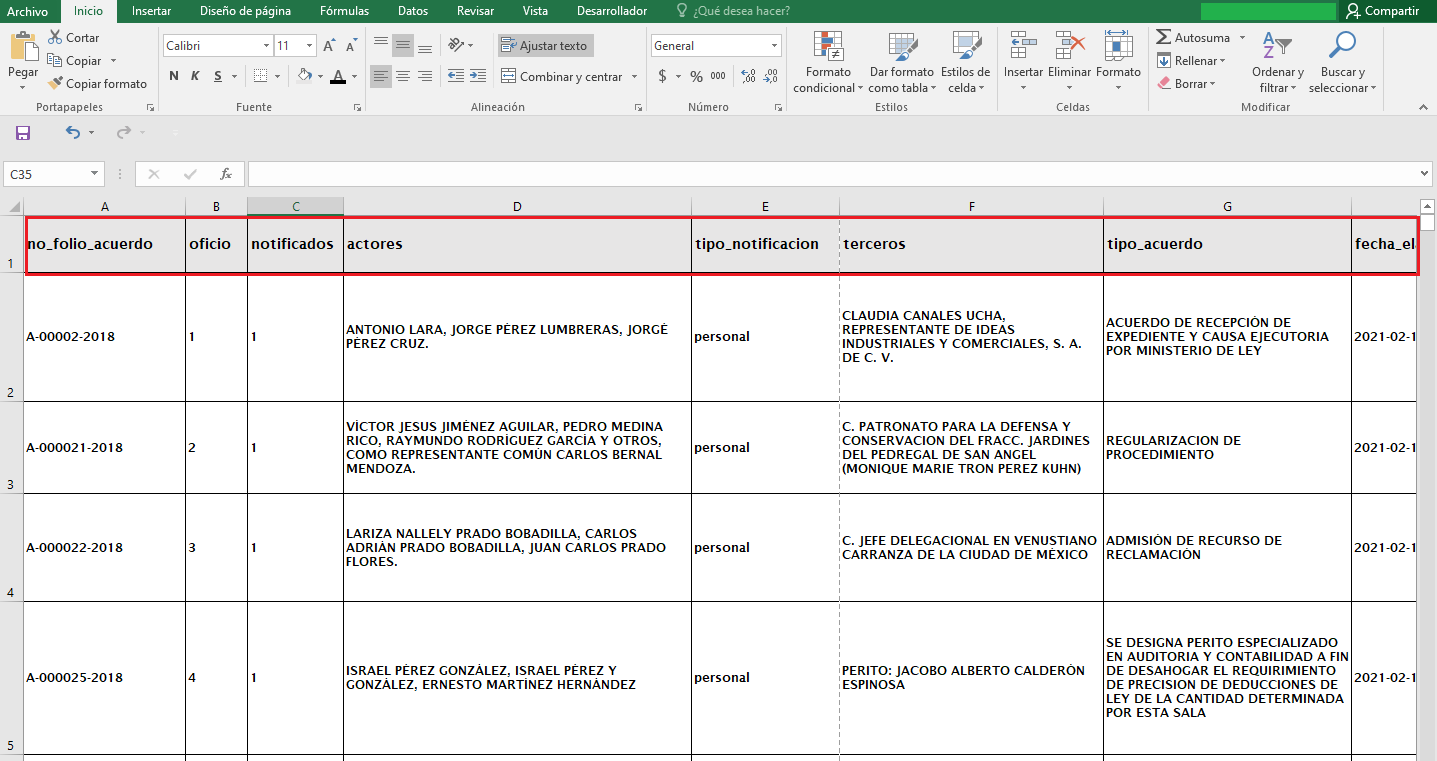
\includegraphics[width=.80\columnwidth]{EJEM.png}
\end{center}

Los campos de:

\begin{itemize}
    \item  actores
    \item  autorizados
\end{itemize}


Se requiere que sean {{\bf separados por coma, cada nombre}} ejemplo de {{\bf actores}}:\\

\begin{center}
    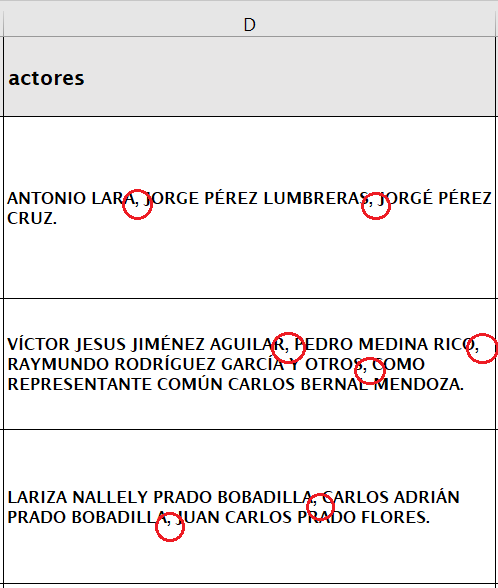
\includegraphics[width=.50\columnwidth]{act.png}
\end{center}

ejemplo de {{\bf autorizados}}:\\

\begin{center}
    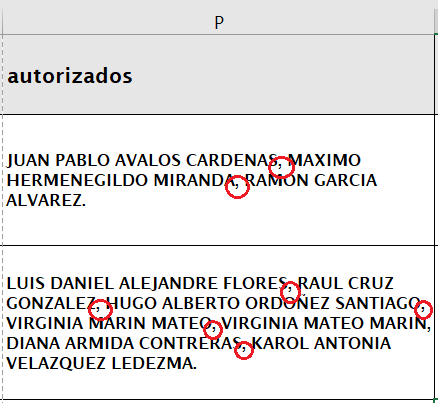
\includegraphics[width=.50\columnwidth]{aut.png}
\end{center}

Los campos de

\begin{itemize}
    \item  fecha\_elaboracion\_acuerdo
    \item  fecha\_elaboracion\_cedula
    \item  fecha\_entrega\_actuaria
\end{itemize}


Tienen que tener el formato de {{\bf AÑO-MES-DÍA  }}
Ejemplo:

\begin{center}
    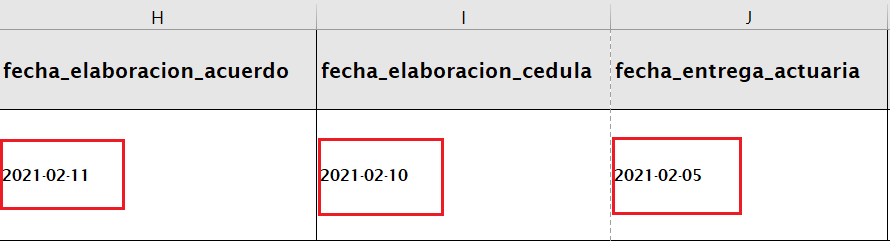
\includegraphics[width=0.60\columnwidth]{formato.png}
\end{center}

Teniendo nuestro archivo con el formato correcto, daremos click en el botón  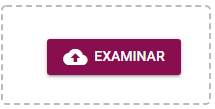
\includegraphics[width=0.15\columnwidth]{examinar.png}
automáticamente se nos abrirá una ventana donde seleccionaremos nuestro archivo de Excel y daremos click en el botón {\bf{ <<Abrir>>}}

\begin{center}
    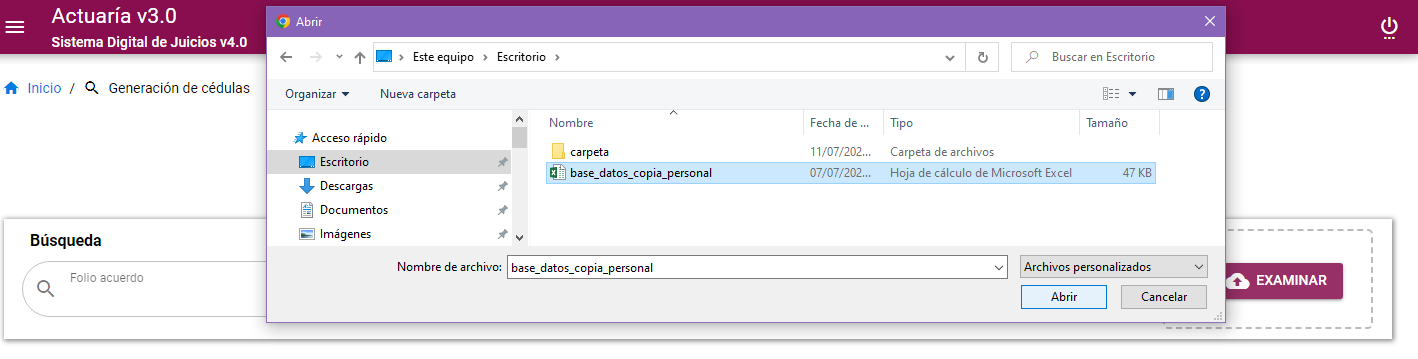
\includegraphics[width=0.90\columnwidth]{exam2.png}
\end{center}

El sistema mostrará la siguiente pantalla:
\begin{center}
    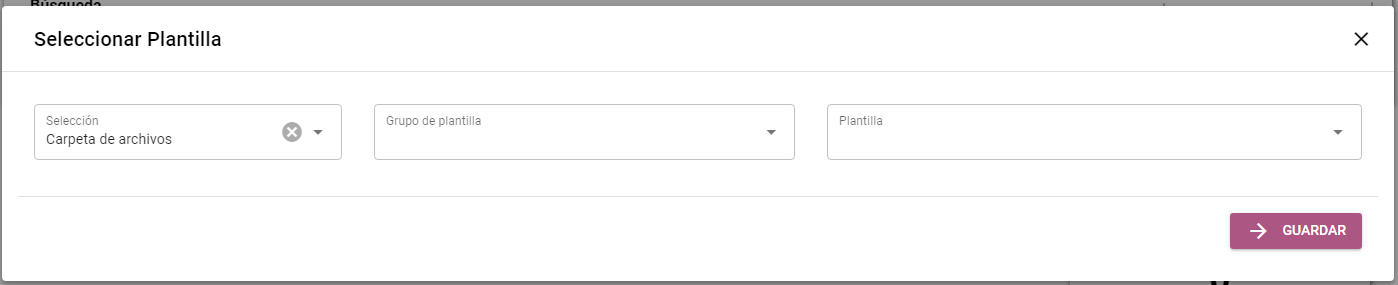
\includegraphics[width=0.90\columnwidth]{select.png}
\end{center}

Seleccionaremos :
\begin{itemize}
    \item  Carpeta
    \item  Grupo de plantilla
    \item  Plantilla
\end{itemize}

En caso de no contar con una plantilla registrada en el sistema, se puede subir una plantilla
temporal.\\
Primero tienes que seleccionar: Subir archivo y dar click en subir archivo para que abra la ventana para seleccionar archivo.

\begin{center}
    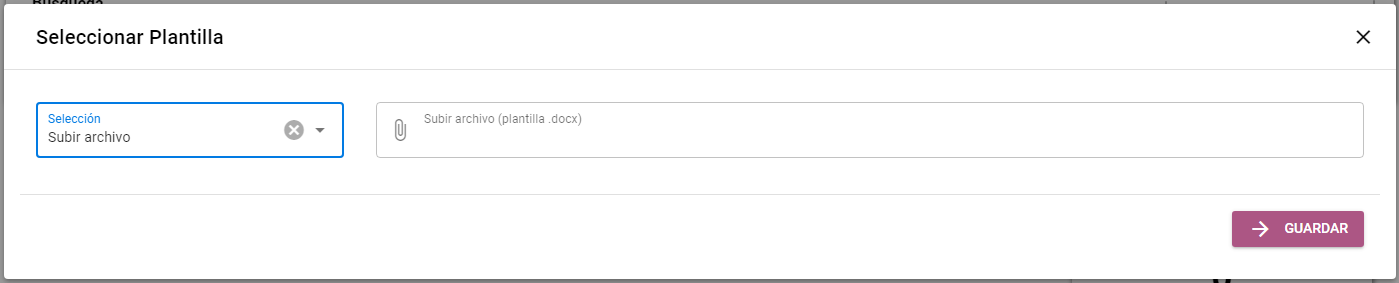
\includegraphics[width=0.90\columnwidth]{select2.png}
\end{center}

Después de ingresar los datos daremos click en el botón
{\bf{
<<SIGUIENTE>>}}\\
Nos aparecerá una alerta con el estatus de los acuerdos ingresados por el excel, en este caso de ejemplo 
podemos ver que dice que se cargaron 0 acuerdos correctamente, por lo tanto hay 5 acuerdos con errores y 
nos menciona que podemos ver los errores dando click en el icono     

\includegraphics[width=.05\columnwidth]{icob.png}

\begin{center}
    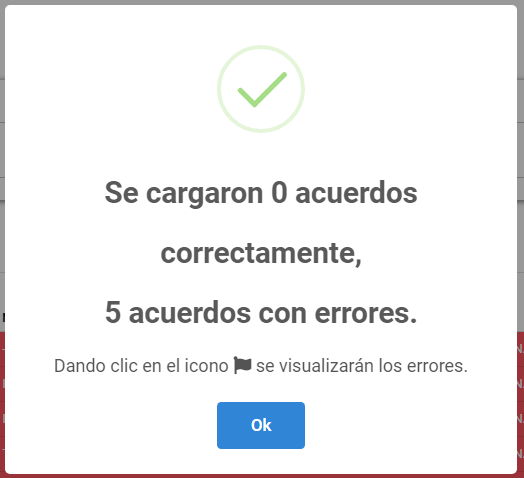
\includegraphics[width=0.50\columnwidth]{alert2.png}
\end{center}

En el caso de tener errores los acuerdos se marcaran en rojo y recorriendo la barra de abajo nos aparecerá el icono de bandera
como en el siguiente ejemplo:

\begin{center}
    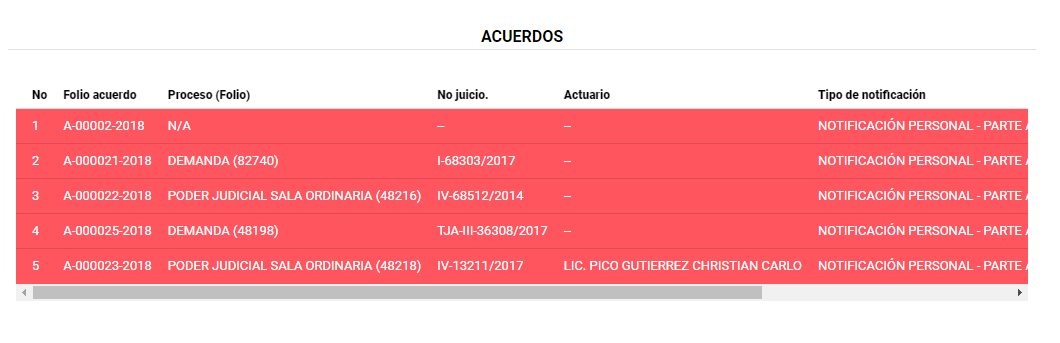
\includegraphics[width=0.90\columnwidth]{bandera.png}
\end{center}

Al recorrer la barra podemos observar el icono de bandera

\begin{center}
    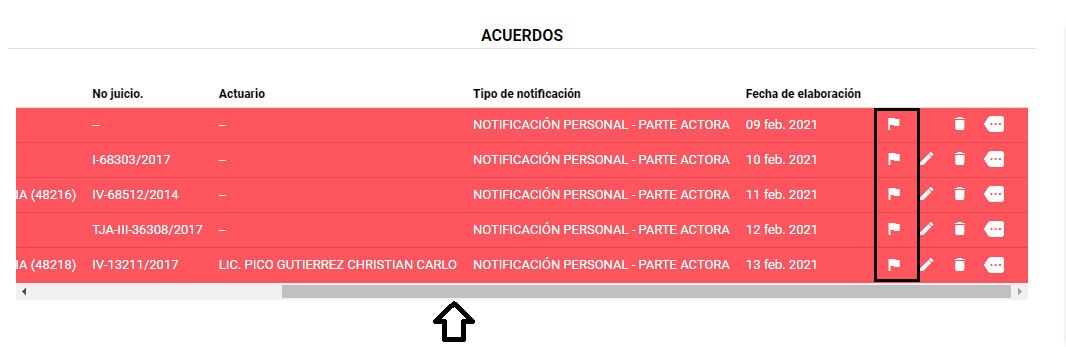
\includegraphics[width=0.90\columnwidth]{bandera2.png}
\end{center}

Al seleccionar el icono podemos ver el error como a continuación.

\begin{center}
    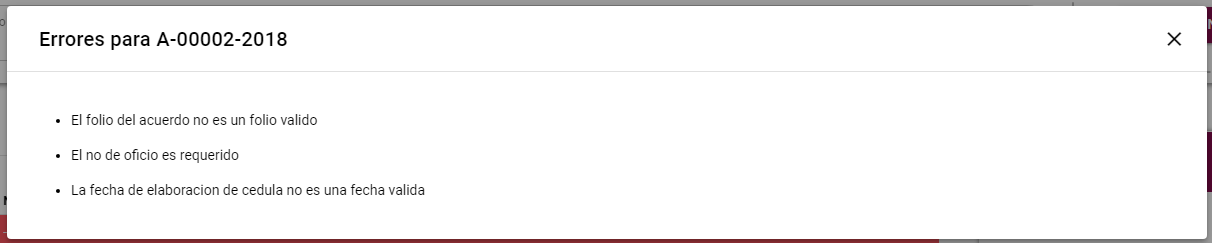
\includegraphics[width=0.90\columnwidth]{errores.png}
\end{center}

Podemos ver que :\\
\begin{itemize}
	\item El folio del acuerdo no es un folio valido\\
	\item El no de oficio es requerido\\
	\item La fecha de elaboración de cédula no es una fecha valida \\ 
\end{itemize}

\vspace{1em}

En este caso tenemos dos opciones:
\begin{enumerate}[1.]
    \item Usar las opciones de corrección del sistema.
    \item Borrar y volver a subir el archivo corregido
\end{enumerate}

\vspace{1cm}

{{\bf1. Usar las opciones de corrección del sistema}}\\
Para solucionar los errores del ejemplo.

El sistema nos permite  {{\bf<<Editar el folio de acuerdo>>}}
dando click en el Folio acuerdo

\begin{center}
    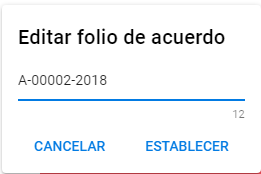
\includegraphics[width=0.40\columnwidth]{edifolio.png}
\end{center}

Después de ingresar el dato correcto daremos click en {{\bf
<<ESTABLECER>>}} el sistema automáticamente verificará si es correcto o no, en caso de error seguirá marcado con rojo.\\
Ahora utilizando el icono {{\bf<<EDITAR>>}}
podemos agregar el número de oficio y editar la fecha.\\

Daremos click en el icono  <<Editar>>

\begin{center}
    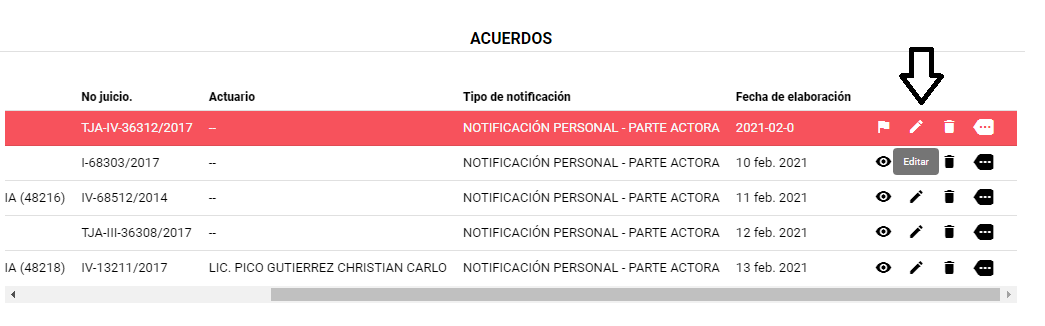
\includegraphics[width=.90\columnwidth]{editarac.png}
\end{center}

El cual nos abrirá la siguiente ventana:

\begin{center}
    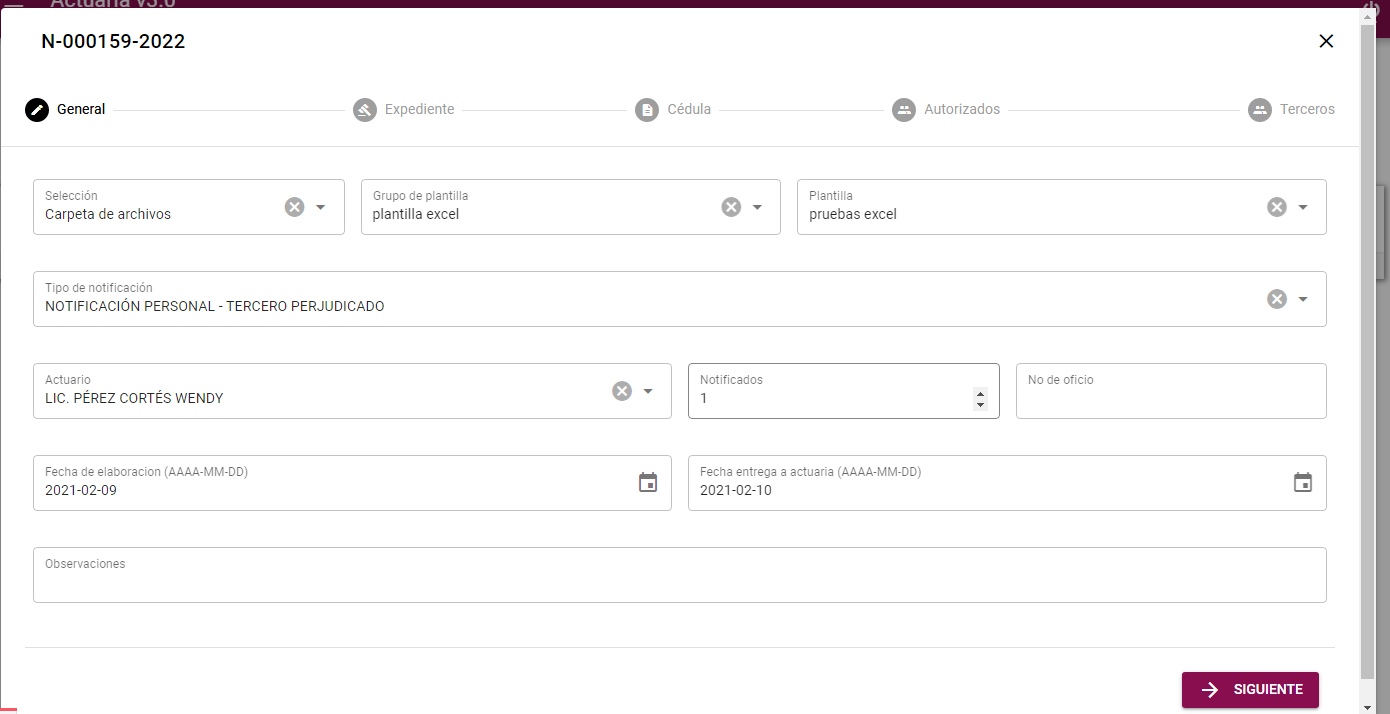
\includegraphics[width=.90\columnwidth]{editaracuerdo.png}
\end{center}

Nos ubicará en  <<General>> aquí
ingresaremos el número de oficio y corregiremos la fecha de elaboración de célula.\\
Daremos click en el botón  {{\bf<<SIGUIENTE>>}} nos aparecerá la siguiente ventana:

\begin{center}
    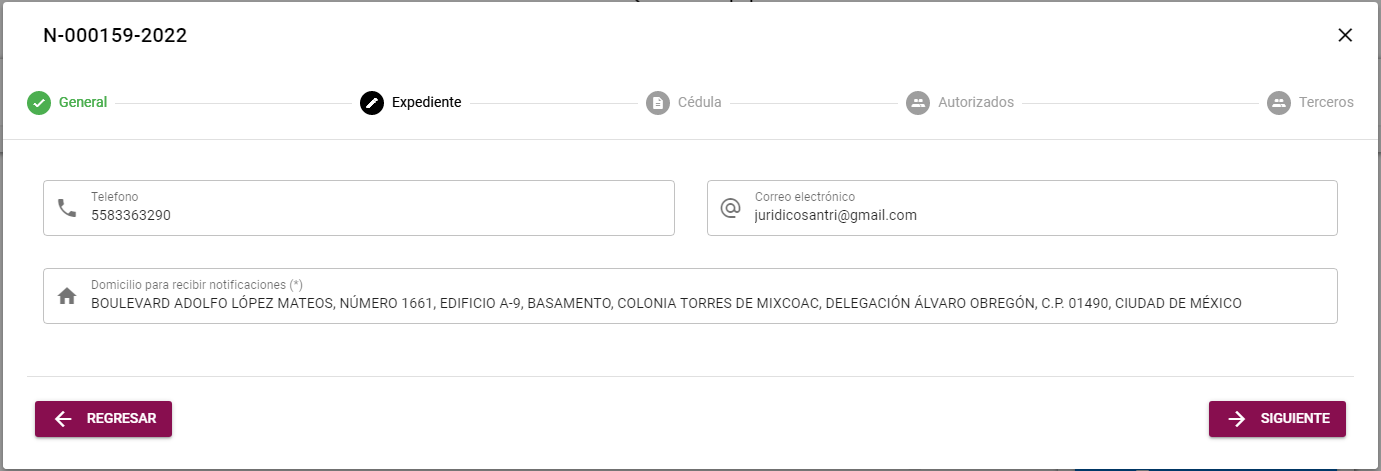
\includegraphics[width=.90\columnwidth]{editaracuerdo2.png}
\end{center}

Podemos revisar nuestros datos o corregir el deseado y
daremos click en el botón  {{\bf<<SIGUIENTE>>}} nos aparecerá la siguiente ventana:

\begin{center}
    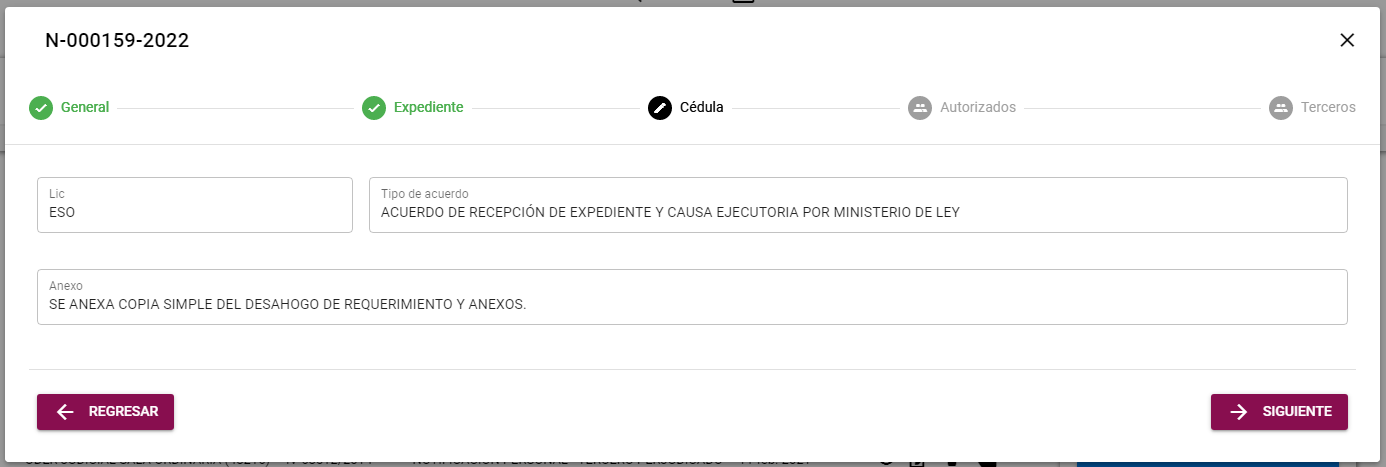
\includegraphics[width=.90\columnwidth]{editaracuerdo3.png}
\end{center}

De igual forma podemos revisar nuestros datos o corregir el deseado y
daremos click en el botón  {{\bf<<SIGUIENTE>>}}
nos aparecerá la siguiente ventana:

\begin{center}
    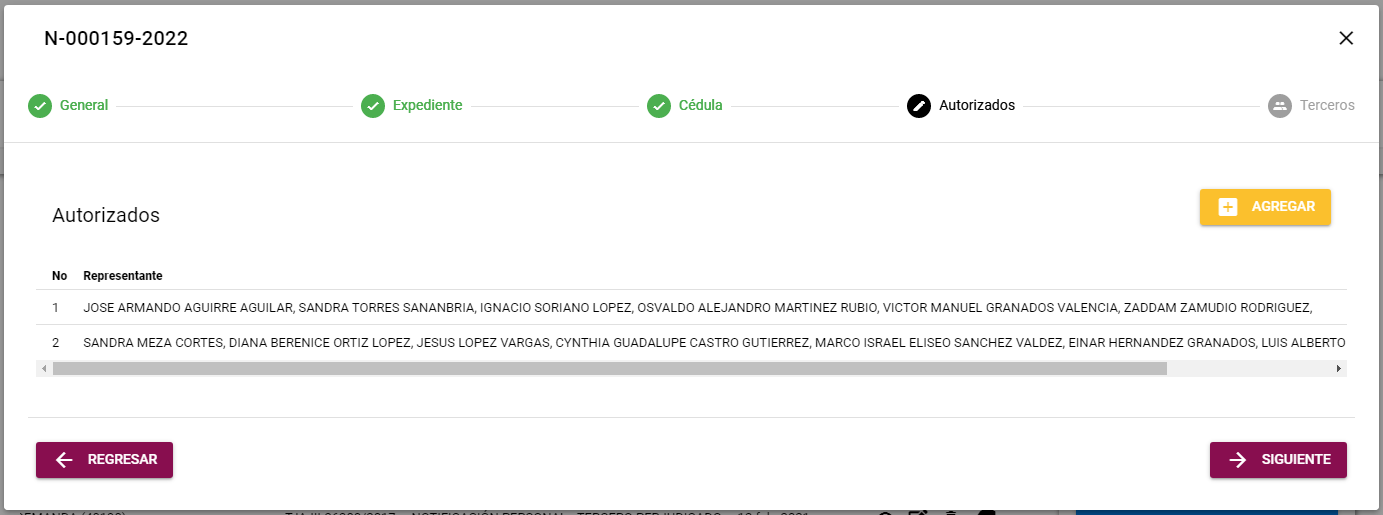
\includegraphics[width=.90\columnwidth]{editaracuerdo4.png}
\end{center}

daremos click en el botón  {{\bf<<SIGUIENTE>>}} nos aparecerá la siguiente ventana:

\begin{center}
    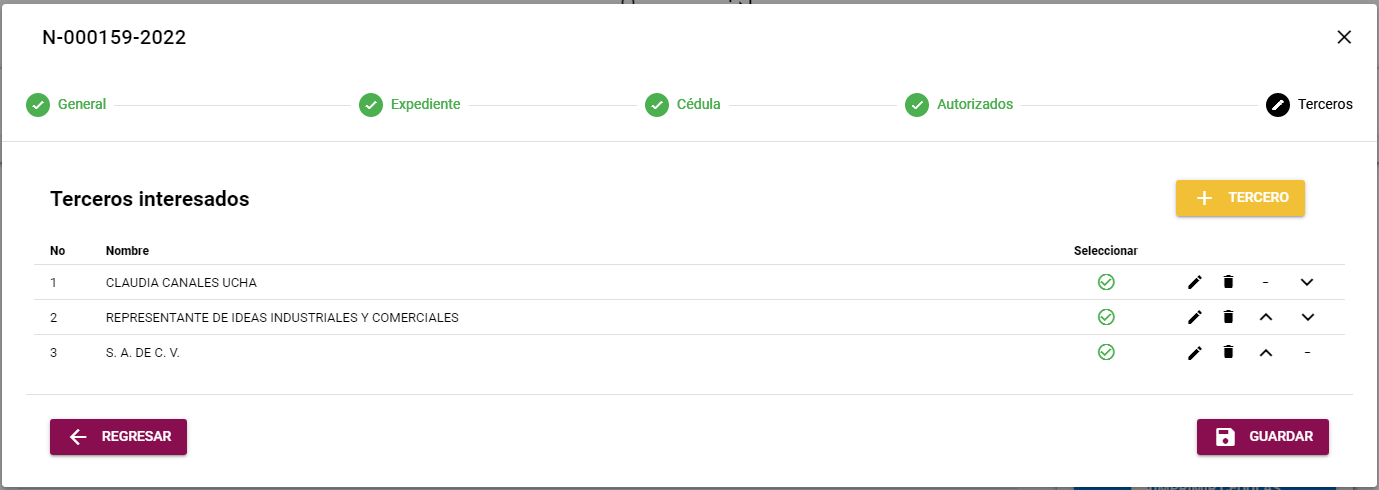
\includegraphics[width=.90\columnwidth]{editaracuerdo5.png}
\end{center}

Daremos click en el botón {{\bf <<GUARDAR>>}} si los datos de nuestros acuerdos son correctos
nos aparecerá el siguiente mensaje

\begin{center}
    
\includegraphics[width=.30\columnwidth]{cedulaguardada.png}
\end{center}

Seguido de este mensaje.
\begin{center}
    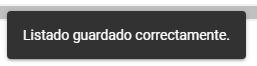
\includegraphics[width=.33\columnwidth]{listadoguardado.png}
\end{center}

Ahora ya podemos visualizar nuestros acuerdos corregidos.

\begin{center}
    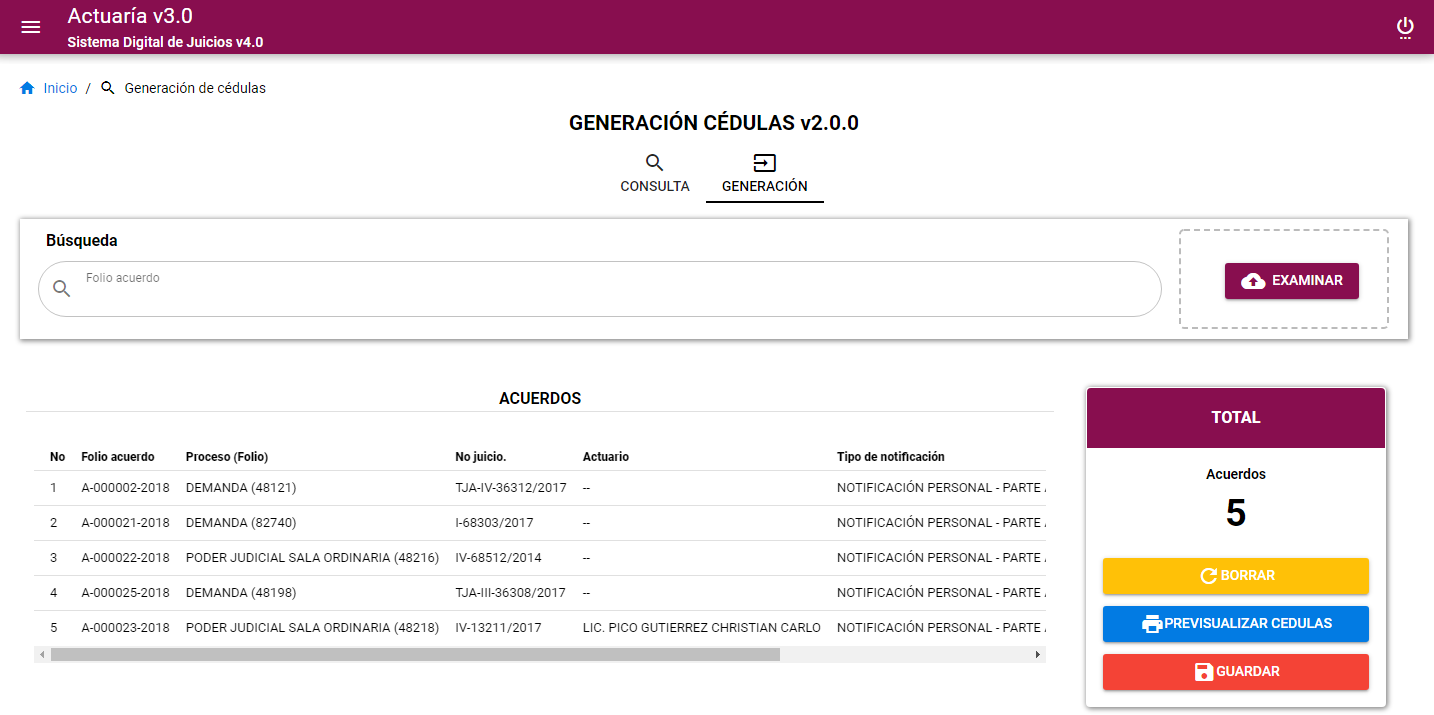
\includegraphics[width=0.90\columnwidth]{corregido.png}
\end{center}

Si lo deseamos podemos:\\
{{\bf
<<PRE VISUALIZAR CÉDULAS>> \\
<<BORRAR>> \\
<<GUARDAR>>
}}


\vspace{1cm}
2.{{\bf Borrar y volver a subir el archivo corregido}}\\
Daremos click en el botón <<Borrar>>

\begin{center}
    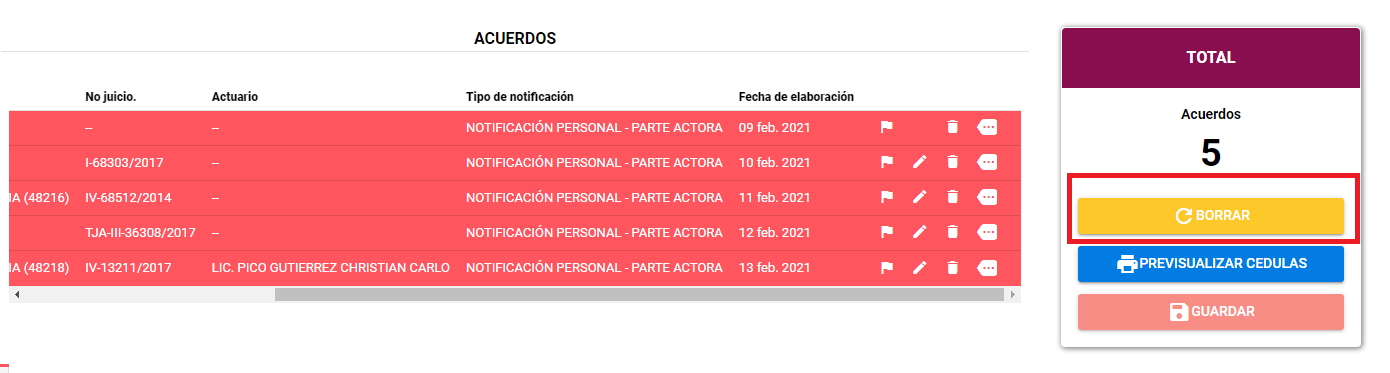
\includegraphics[width=0.90\columnwidth]{borraracuerdos.png}
\end{center}

Nos aparecerá una alerta:
\begin{center}
    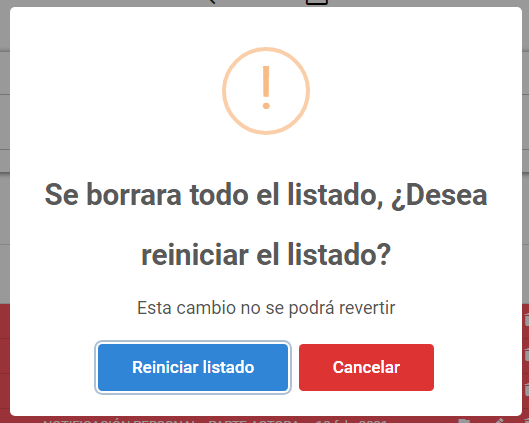
\includegraphics[width=0.50\columnwidth]{reiniciarlis.png}
\end{center}

Daremos click en {{\bf<<Reiniciar listado>>}} en caso contrario daremos click en <<Cancelar>>
nos aparecerá la pantalla sin nuestros acuerdos.

\begin{center}
    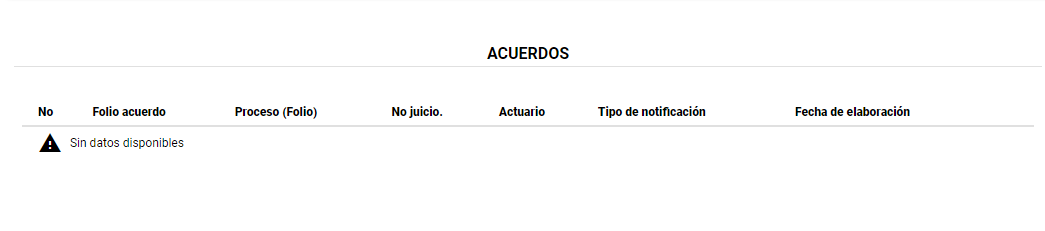
\includegraphics[width=0.90\columnwidth]{sindatos.png}
\end{center}

{\Huge{\color{myblue} \section{Lista de cédulas}\label{sec:14}}}
Para generar un listado de cédulas agregaremos los folios deseados, por cada folio 
agregado el sistema mostrara la siguiente ventana:

\begin{center}
    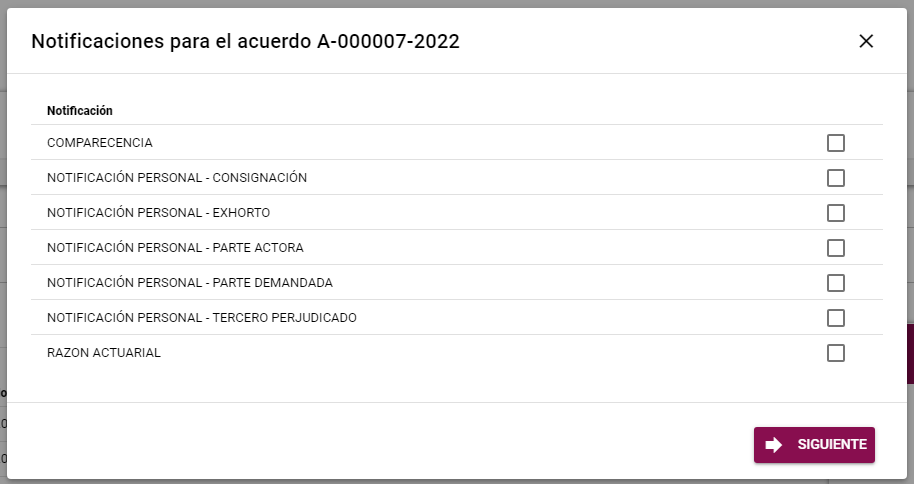
\includegraphics[width=0.80\columnwidth]{lista1.png}
\end{center}

Seleccionaremos las opciones deseadas y daremos click en el botón <<SIGUIENTE>>

Ahora llenaremos el formulario con los siguientes
datos:

\begin{center}
    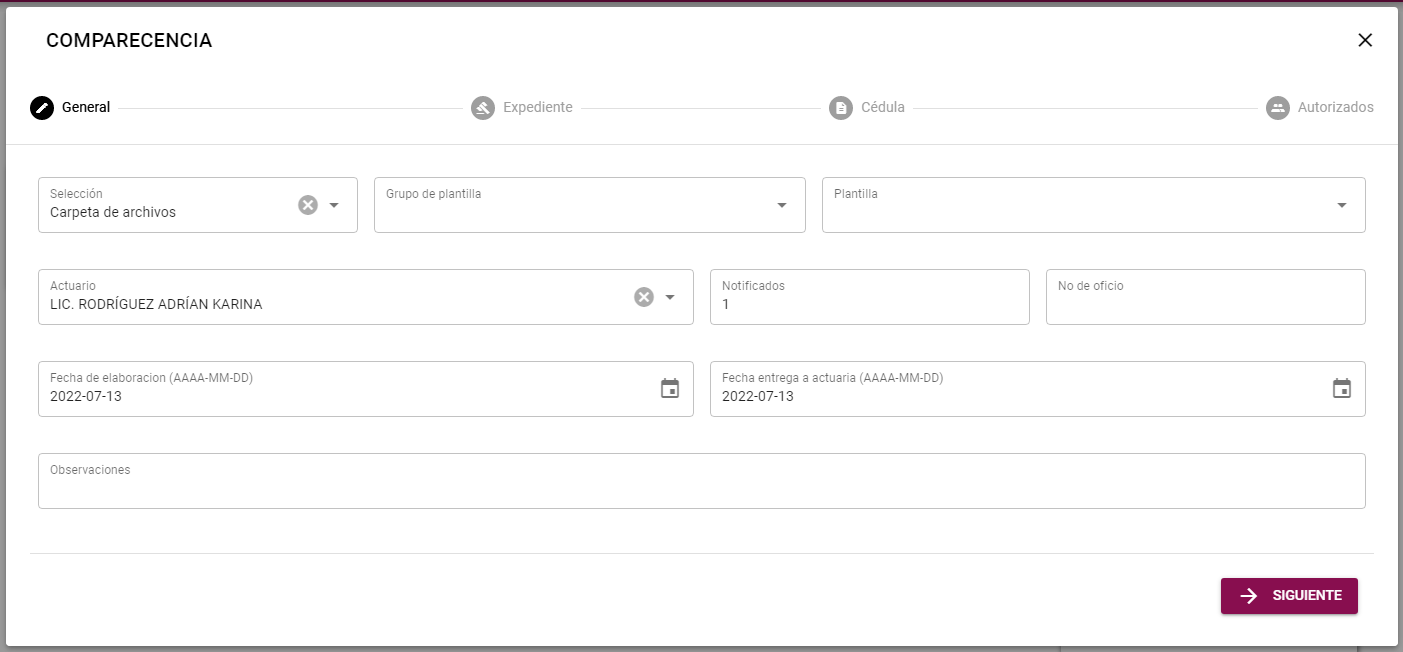
\includegraphics[width=.90\columnwidth]{comparecencia.png}
\end{center}

\begin{itemize}
    \item Selección
    \item  Grupo de plantilla
    \item  Plantilla
    \item  Actuario
    \item  Notificados
    \item  No de oficio
    \item  Fecha entrega a actuaria
    \item  Fecha de elaboración
    \item Observaciones
\end{itemize}

En caso de no contar con una plantilla registrada en el sistema, se puede subir una plantilla
temporal.\\
Primero tienes que seleccionar:
{\bf{<<Subir archivo>>}}y dar click en subir archivo.\\

\begin{center}
    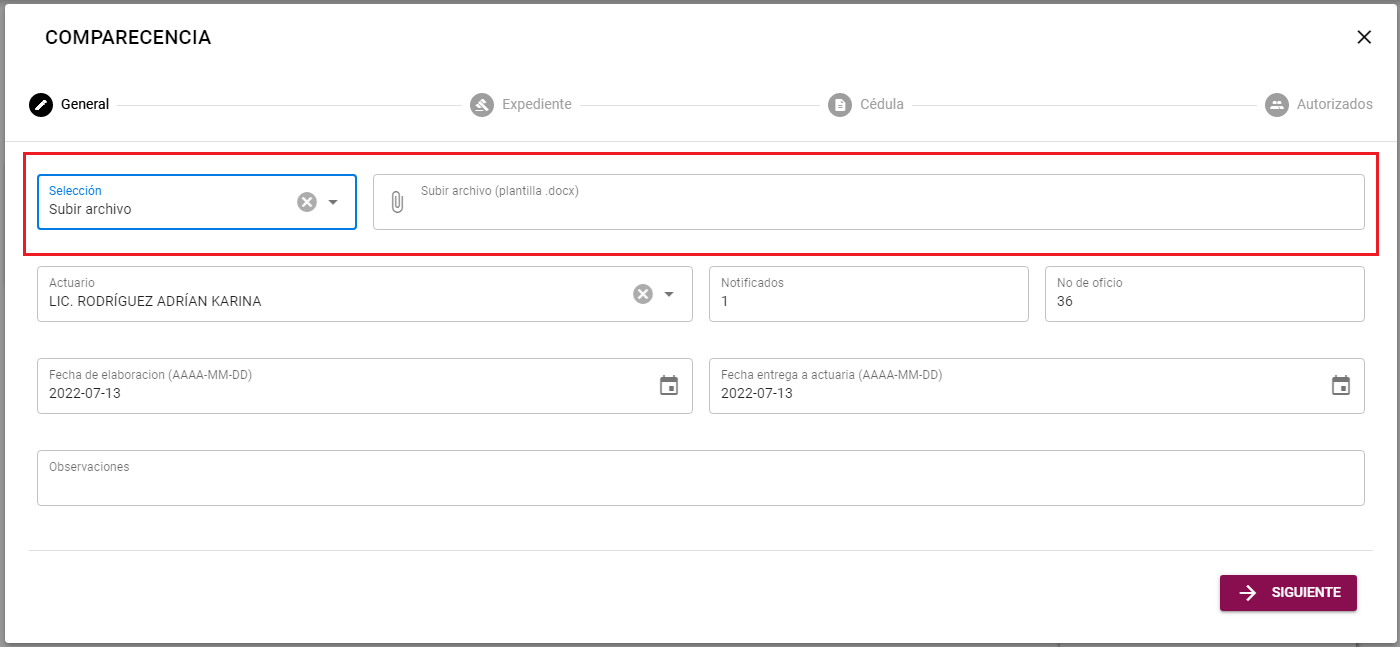
\includegraphics[width=0.90\columnwidth]{comparecencia3.png}
\end{center}

Automáticamente se abrirá una ventana donde seleccionaras tu plantilla desde tus documentos.

\begin{center}
    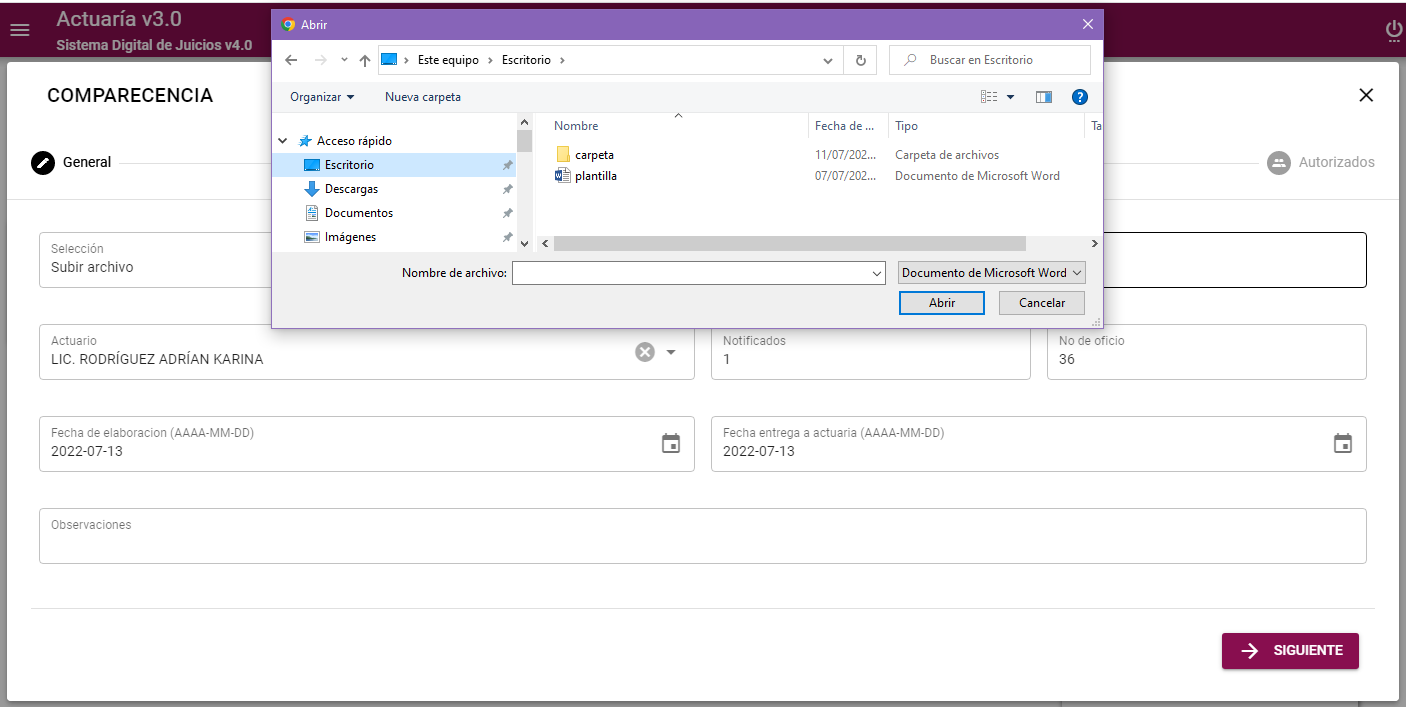
\includegraphics[width=0.90\columnwidth]{comparecencia4.png}
\end{center}

Después de ingresar los datos daremos click en el botón.
{\bf{<<SIGUIENTE>>}}
Ahora ingresaremos los siguientes datos:

\begin{itemize}
    \item Teléfono
    \item Correo electrónico
    \item Domicilio para recibir notificaciones (*) 
\end{itemize}

\begin{center}
    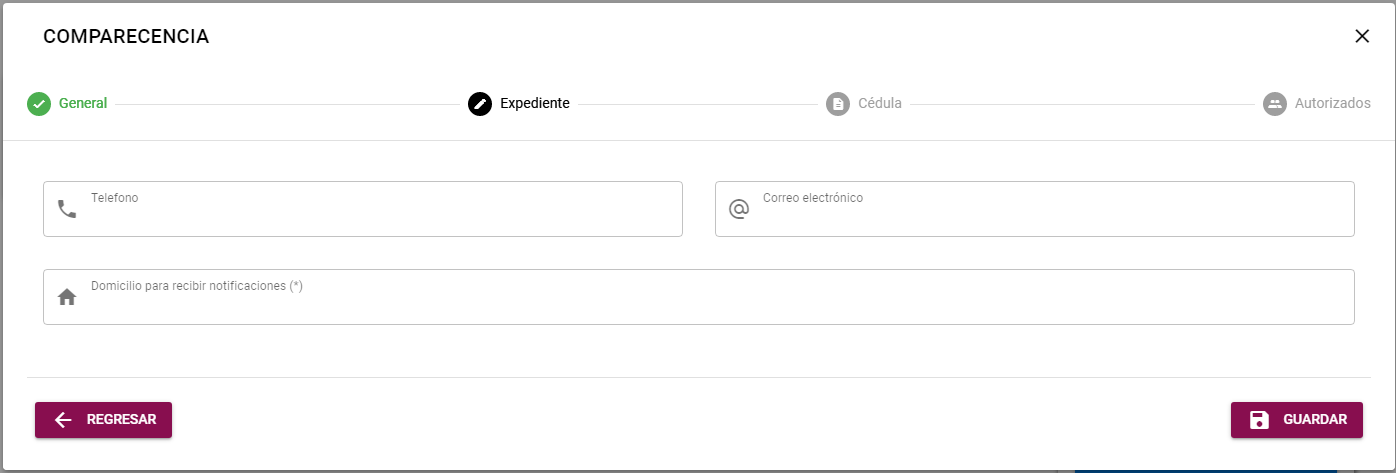
\includegraphics[width=.90\columnwidth]{comparecencia2.png}
\end{center}

Daremos click en {\bf{<<GUARDAR>>}}\\

Después llenaremos los siguientes datos:
\begin{center}
    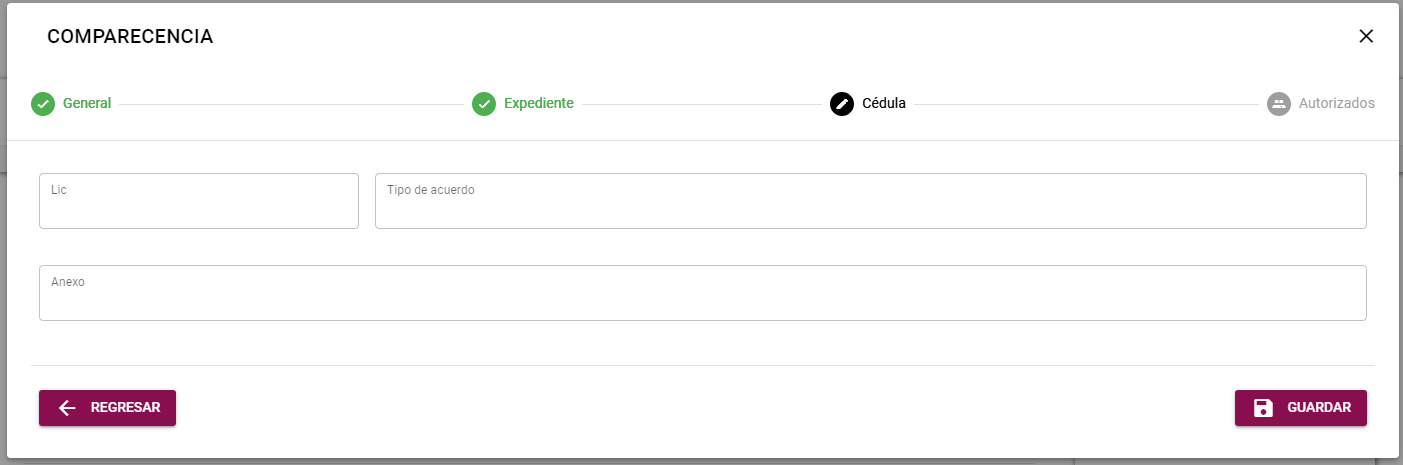
\includegraphics[width=0.90\columnwidth]{lista2.png}
\end{center}

Y daremos click en {\bf{<<GUARDAR>>}}\\

Después podemos agregar representantes o dar click en <<GUARDAR>>
    
\begin{center}
    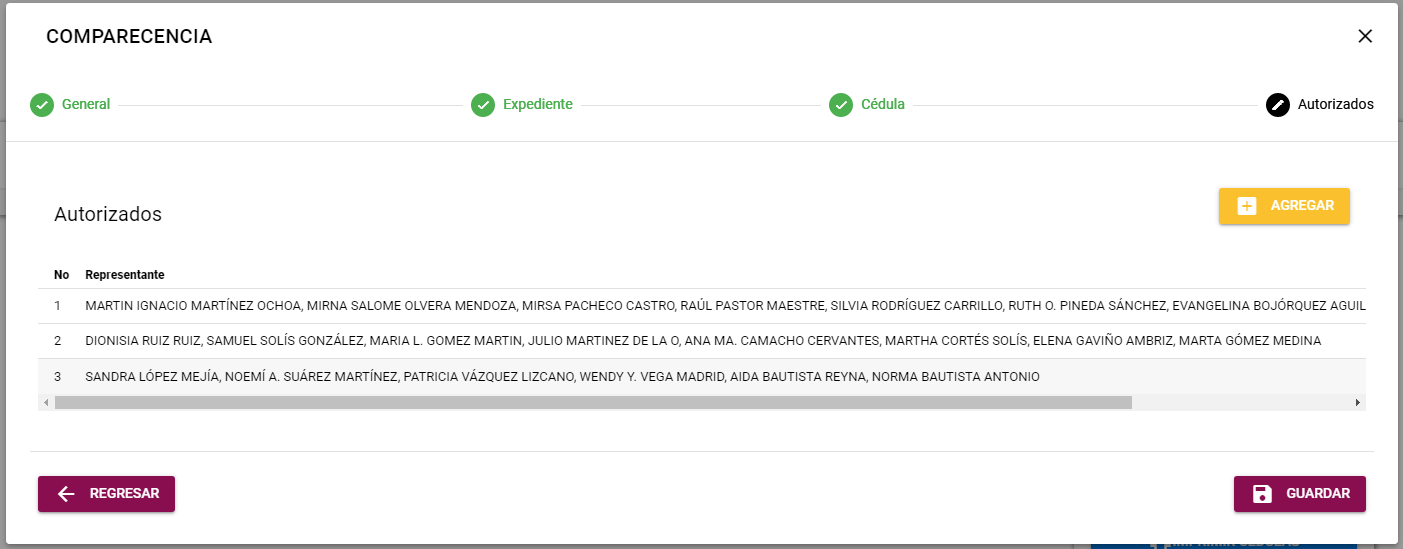
\includegraphics[width=0.90\columnwidth]{lista3.png}
\end{center}

Finalmente daremos click en <<GUARDAR>>.

{\Huge{\color{myblue} \section{Imprimir cédulas}\label{sec:15}}}

Podemos imprimir nuestras cédulas  dando click en el botón <<Imprimir cédulas.>>

\begin{center}
    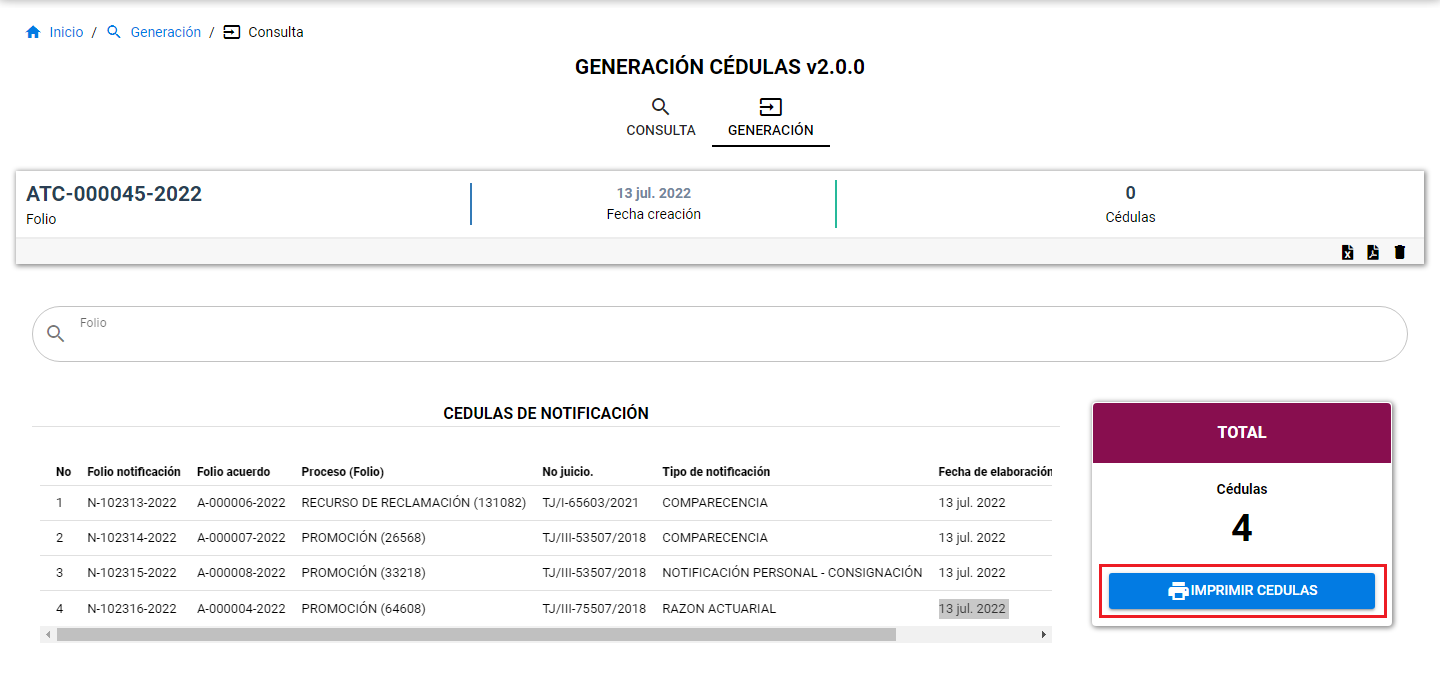
\includegraphics[width=0.88\columnwidth]{imprcedu.png}
\end{center}

Nos aparecerá una ventana donde podemos ver nuestras cédulas con su respectivo código de barras en la parte inferior derecha.

\begin{center}
    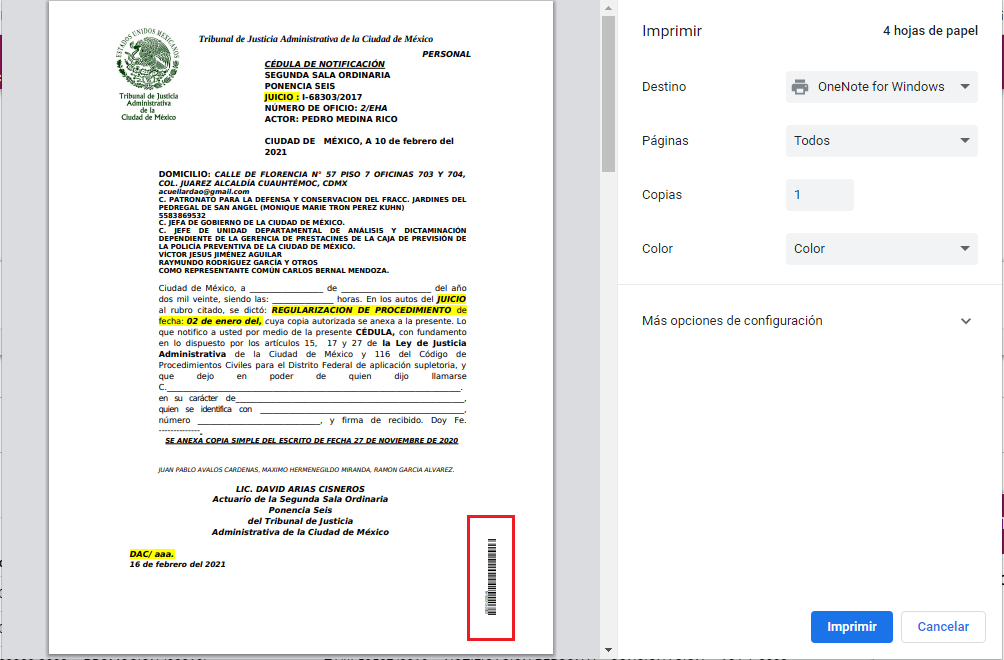
\includegraphics[width=0.90\columnwidth]{impcedula.png}
\end{center}

\newpage

{\Huge{\color{myblue} \section{Acciones}\label{sec:16}}}

Para cada notificación podemos realizar las siguientes acciones.

\begin{center}
    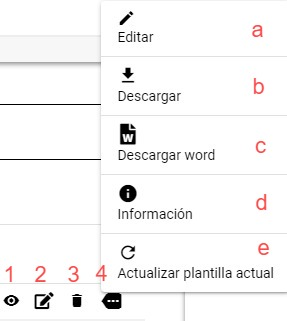
\includegraphics[width=.40\columnwidth]{masf.jpeg}
\end{center}


\begin{enumerate}[(1)]
    \item Visualizar cédula
    \item Editar
    \item Borrar
    \item Más
        \begin{enumerate}[(a)]
            \item Editar
            \item Descargar
            \item Descargar word
            \item Información
            \item Actualizar plantilla actual
        \end{enumerate}
\end{enumerate}


{\Huge{\color{myblue} \section{Visualizar cédula}\label{sec:17}}}
Para poder ver nuestra cédula basta con dar click en el icono (1) y nos mostrará el archivo.
Ejemplo:

\begin{center}
    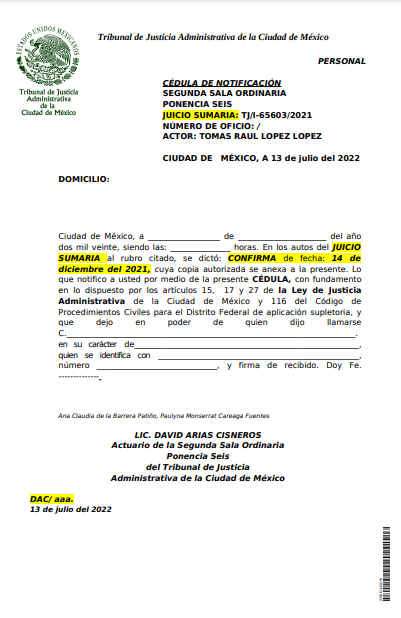
\includegraphics[width=0.77\columnwidth]{cedu.png}
\end{center}

{\Huge{\color{myblue} \section{Editar}\label{sec:18}}}
Para poder editar la cédula daremos click en el icono (2) y nos mostrará la pantalla siguiente con las secciones de

\begin{enumerate}[(1)]
    \item General
    \item Expediente
    \item Cédula
    \item Autorizados
    \item Actores
\end{enumerate}



\begin{center}
    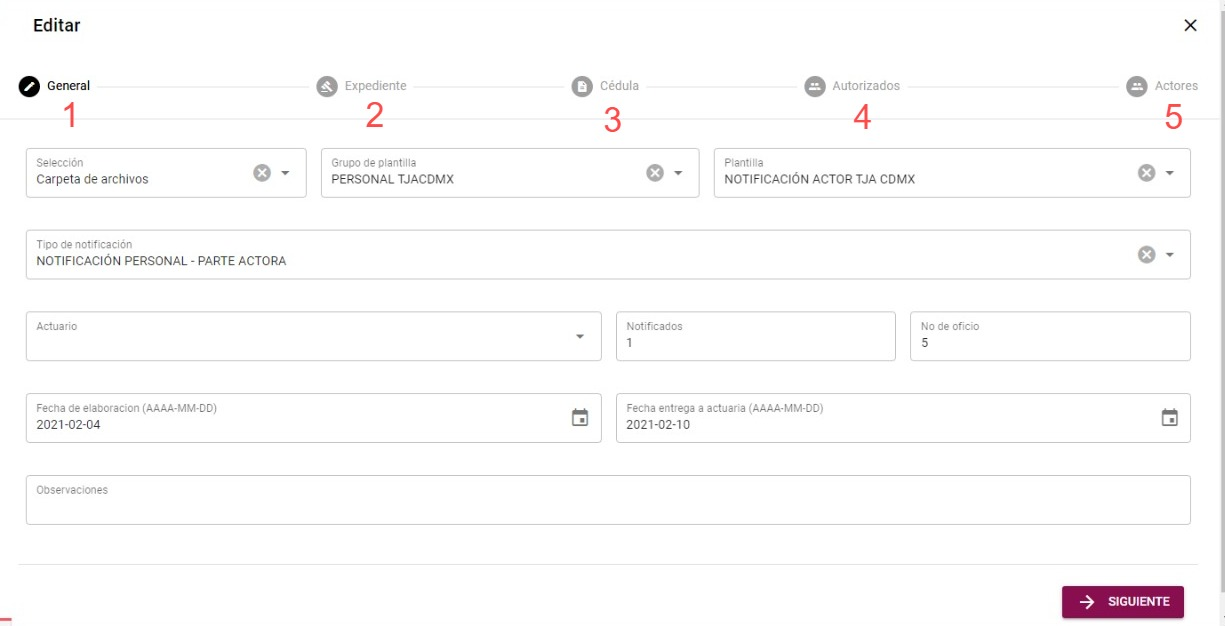
\includegraphics[width=0.90\columnwidth]{editar6.jpeg}
\end{center} En  <<General>>


Aquí ingresaremos los siguientes datos (1)  {\bf{
<<General>>:}}


\begin{enumerate}[(a)]
    \item Selección: Carpeta de archivos o subir archivo
    \item Grupo de plantilla
    \item Plantilla
    \item Tipo de notificación
    \item Actuario
    \item Notificados
    \item No oficio
    \item Fecha entrega a actuaria
    \item Fecha elaboración
    \item Observaciones
\end{enumerate}

Daremos click en el botón  {{\bf<<SIGUIENTE>>}}
nos aparecerá la siguiente ventana:

\begin{center}
    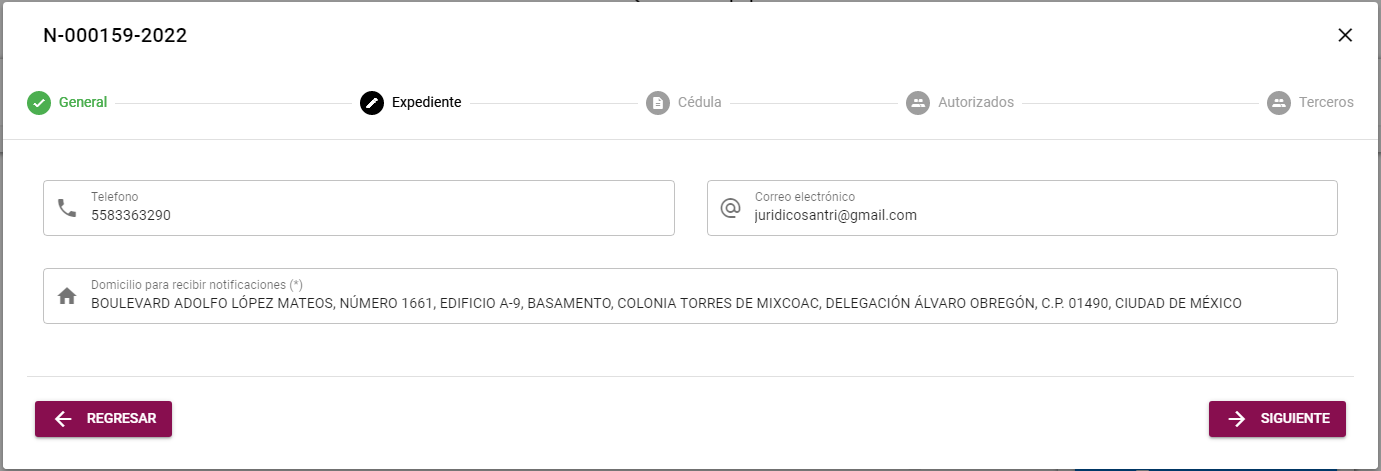
\includegraphics[width=.90\columnwidth]{editaracuerdo2.png}
\end{center}

Podemos revisar nuestros datos o corregir el deseado y
daremos click en el botón  {{\bf<<SIGUIENTE>>}}
nos aparecerá la siguiente ventana:

\begin{center}
    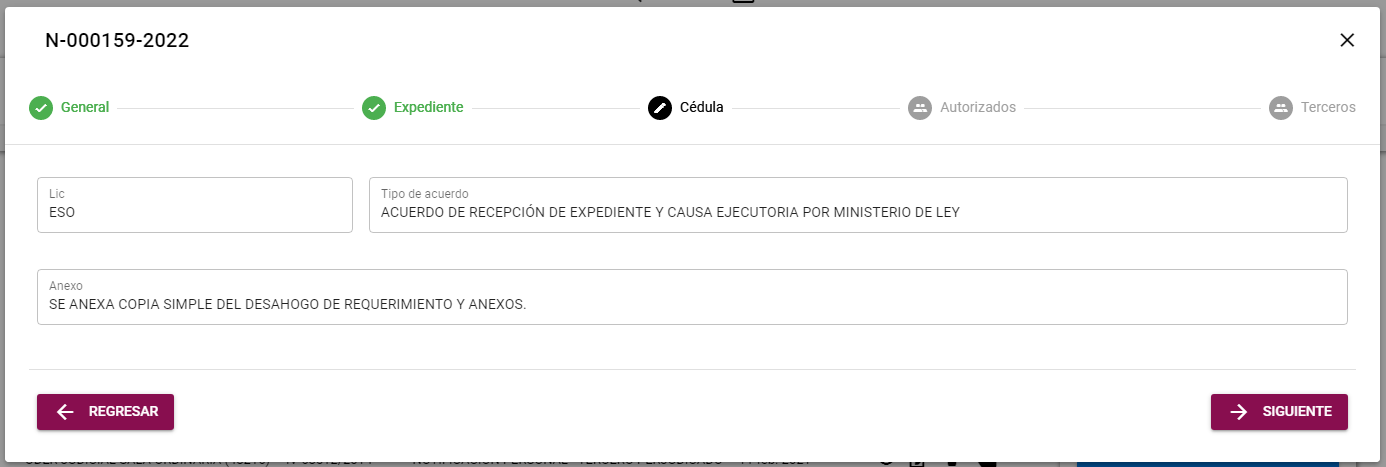
\includegraphics[width=.90\columnwidth]{editaracuerdo3.png}
\end{center}

De igual forma podemos revisar nuestros datos o corregir el deseado y
daremos click en el botón  {{\bf<<SIGUIENTE>>}}
nos aparecerá la siguiente ventana:

\begin{center}
    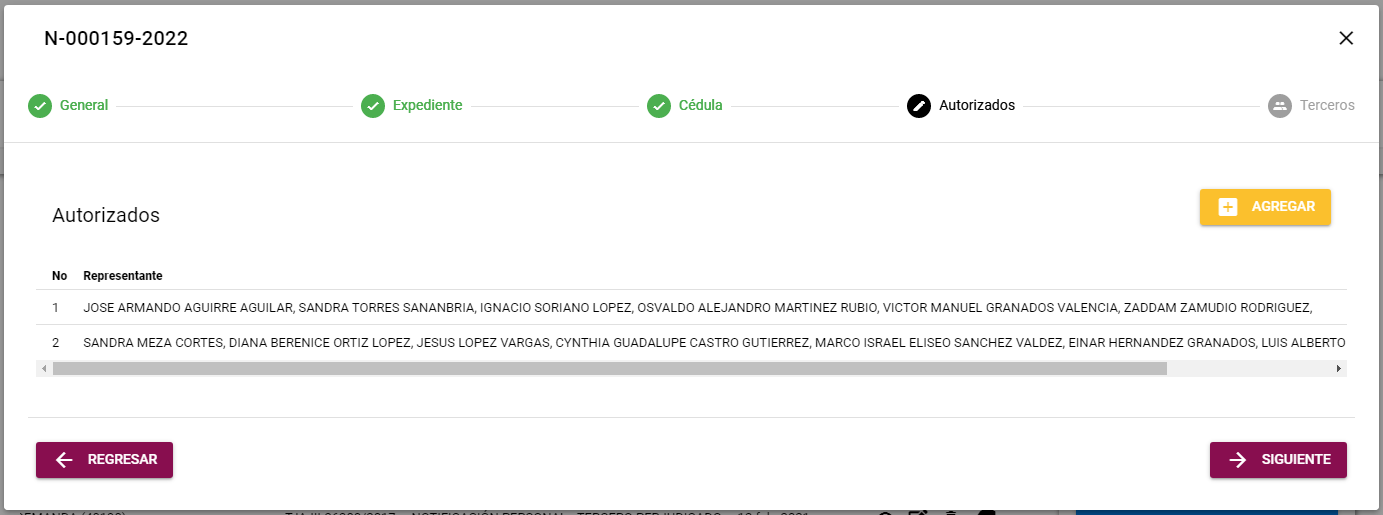
\includegraphics[width=.90\columnwidth]{editaracuerdo4.png}
\end{center}

daremos click en el botón  {{\bf<<SIGUIENTE>>}}
nos aparecerá la siguiente ventana:

\begin{center}
    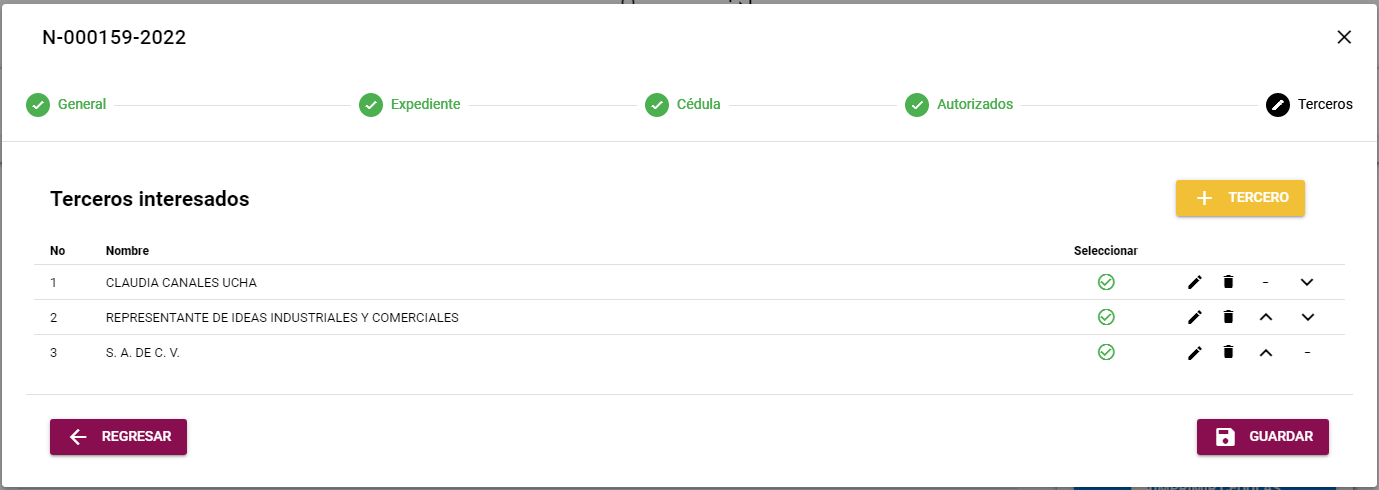
\includegraphics[width=.90\columnwidth]{editaracuerdo5.png}
\end{center}

Daremos click en el botón {{\bf <<GUARDAR>>}} si los datos de nuestros acuerdos son correctos nos aparecerá el siguiente mensaje
\begin{center}
    
\includegraphics[width=.30\columnwidth]{cedulaguardada.png}
\end{center}

Seguido de este mensaje.
\begin{center}
    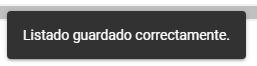
\includegraphics[width=.33\columnwidth]{listadoguardado.png}
\end{center}

Ahora ya podemos visualizar nuestros acuerdos corregidos.
\begin{center}
    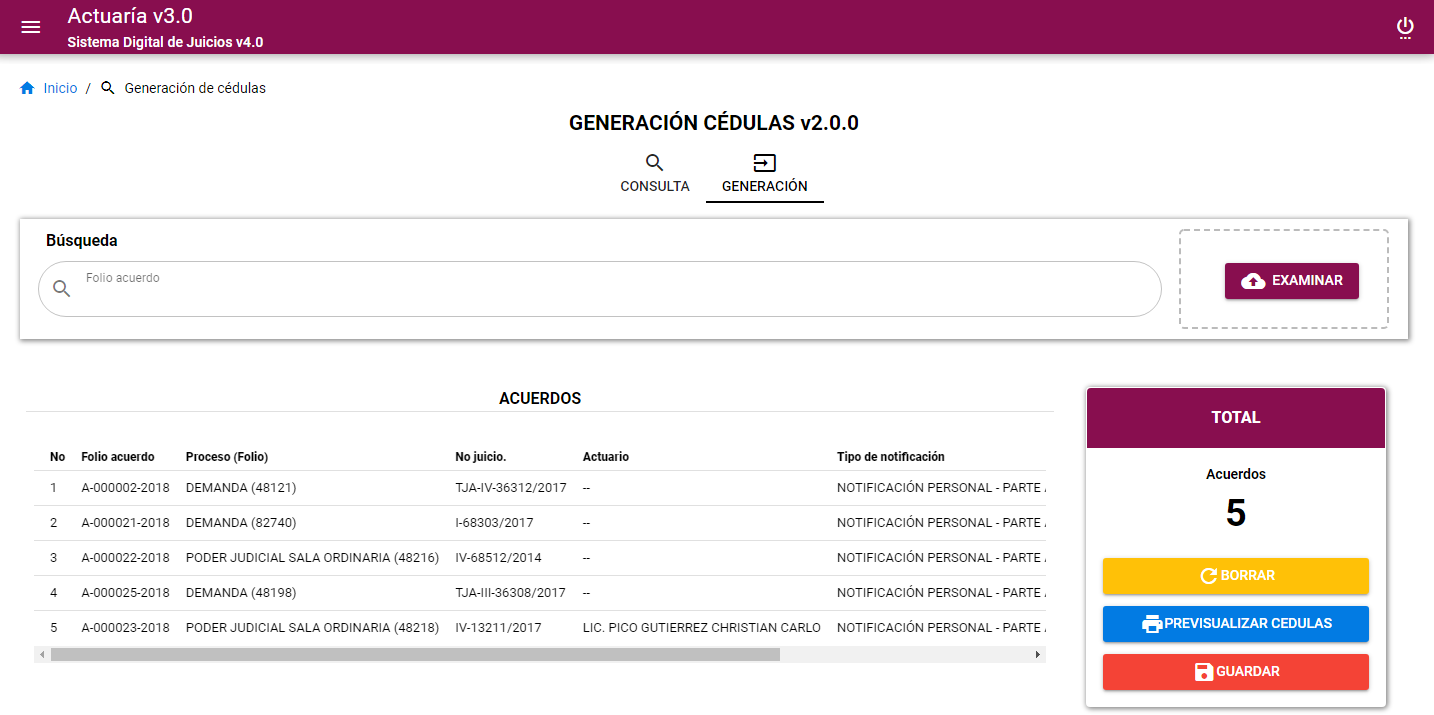
\includegraphics[width=.90\columnwidth]{corregido.png}
\end{center}

Si lo deseamos podemos:\\
{{\bf
<<PREVISUALIZAR CÉDULAS>> \\
<<BORRAR>> \\
<<GUARDAR>>
}}


En caso de no contar con una plantilla registrada en el sistema, se puede subir una plantilla
temporal.\\
Primero tienes que seleccionar:
Subir archivo.\\
y dar click en subir archivo para que abra la ventana para seleccionar archivo.

\begin{center}
    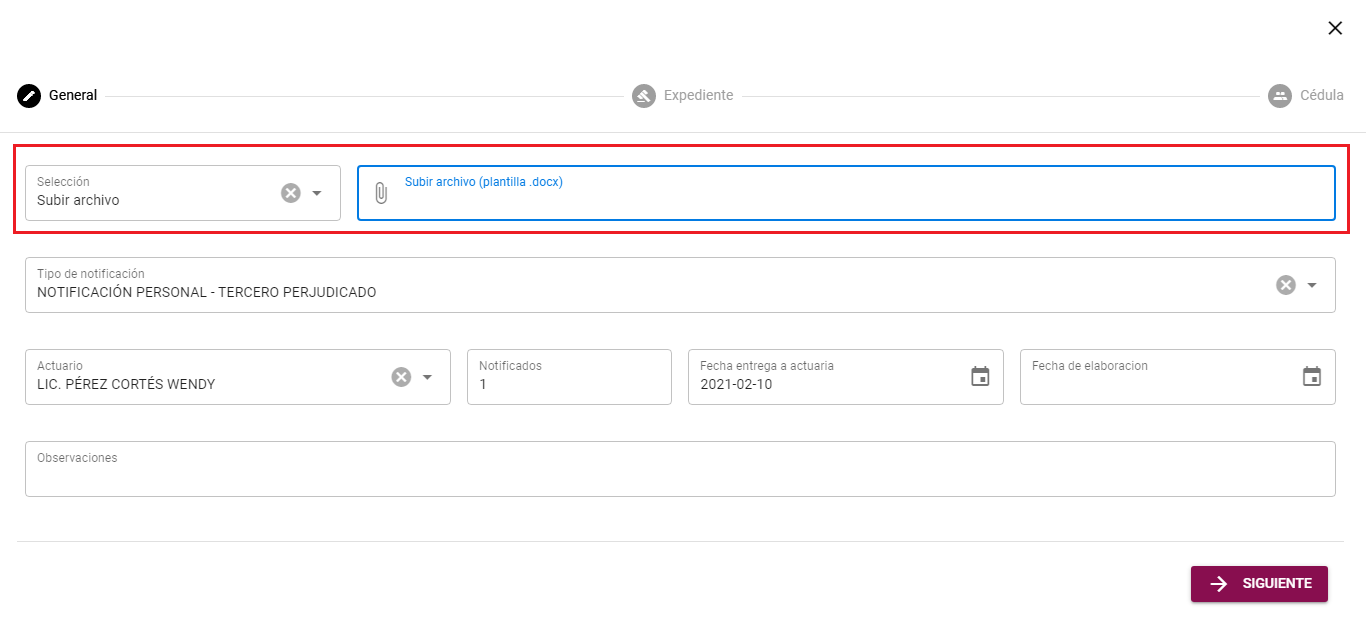
\includegraphics[width=.90\columnwidth]{subira.png}
\end{center}

Después de ingresar los datos daremos click en {\bf{
<<SIGUIENTE>>}}

\begin{center}
    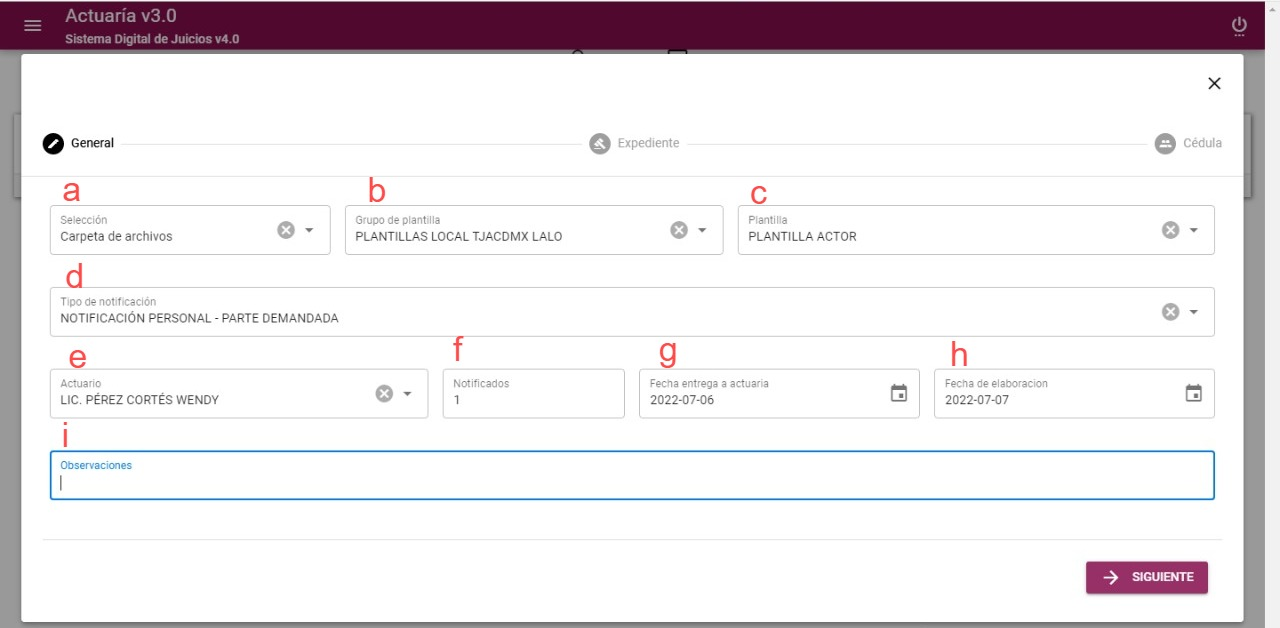
\includegraphics[width=.90\columnwidth]{op2.jpeg}
\end{center}

Ahora ingresaremos: {\bf{Domicilio para recibir notificaciones.}}
\begin{center}
    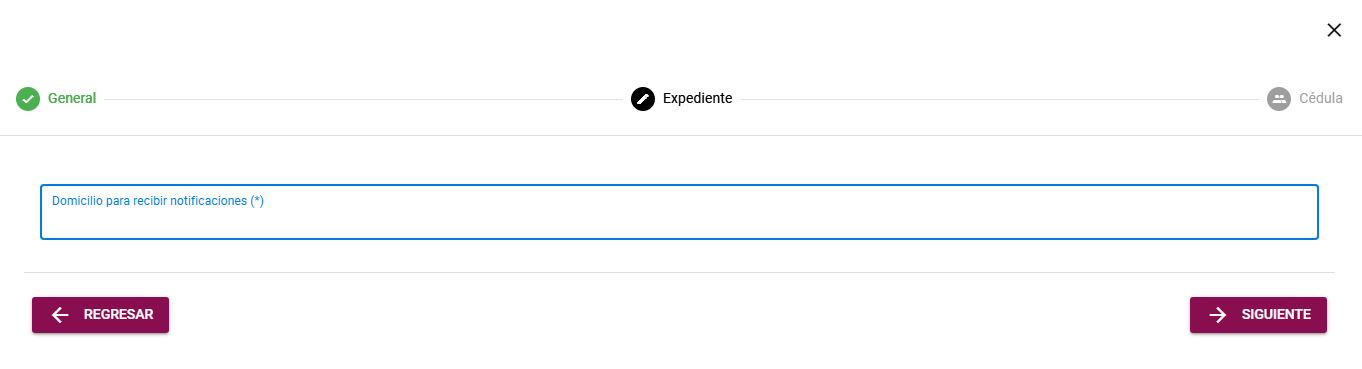
\includegraphics[width=.90\columnwidth]{op3.png}
\end{center}

Daremos click en {\bf{<<SIGUIENTE>>}}
Podemos agregar {\bf{ <<Actor, Autoridad>>}} para  agregar Actor(es)
solo deberá de dar click en el botón  {\bf{ «+ ACTOR»}}, e ingresar la siguiente información:

\begin{itemize}
    \item Tipo de persona.
    \item Nombre.
    \item Apellido paterno.
    \item Apellido materno.
    \item Genero.
    \item Teléfono.
    \item Correo.
    \item Delegación.
    \item Domicilio.
\end{itemize}



\begin{center}
    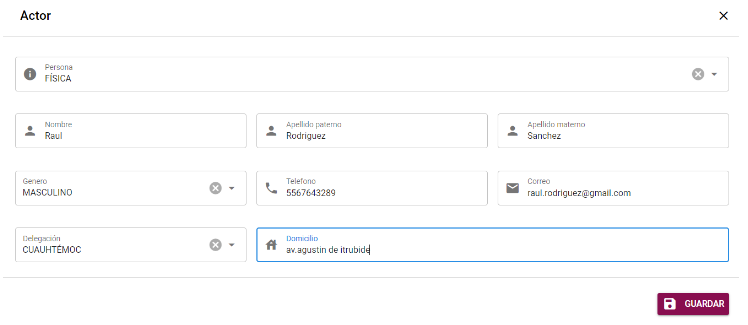
\includegraphics[width=.90\columnwidth]{actor.png}
\end{center}

A continuación, deberá dar click en el botón «GUARDAR», mostrara la lista de los actores registrados.
Para borrar un actor solo debes de dar click en el icono borrar       

\includegraphics[width=.05\columnwidth]{iconob.png}\\
Nos mostrara un mensaje de confirmación,
da click en el botón «BORRAR» si está seguro.\\
El actor se quitará automáticamente de la lista de
actores, en caso de no estar seguro de borrar al actor solo debe de dar click «CANCELAR».\\

Podemos observar las cédulas de notificación registradas, debe de dar click en el botón «GUARDAR» para que
se guarde correctamente el listado, en caso de borrar todo el listado solo debe de dar click el botón
«BORRAR», para que se reinicie el listado.\\
En el caso de Autoridades,
{\bf{<<Autoridades>>}} aquí podemos:

\begin{center}
    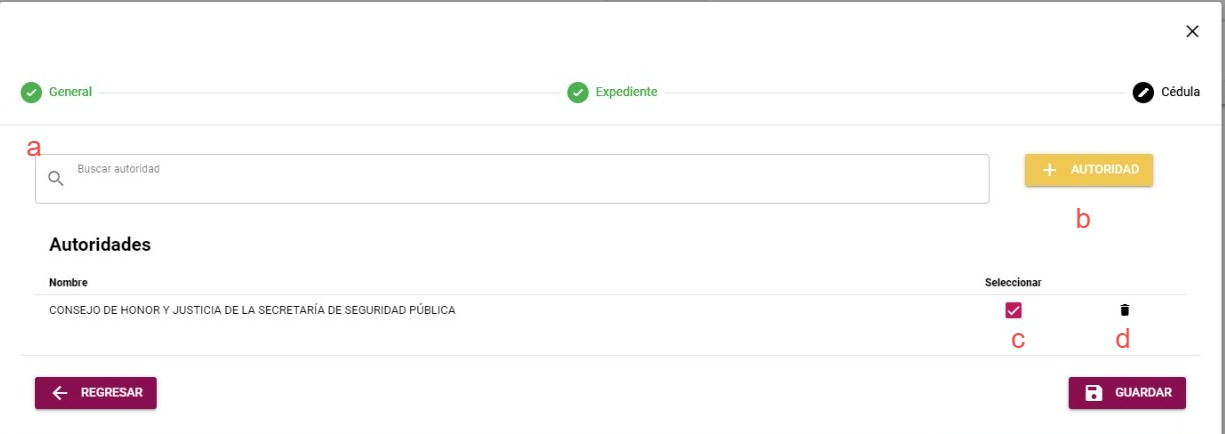
\includegraphics[width=0.90\columnwidth]{op4.jpeg}
\end{center}

\begin{enumerate}[(a)]
 \item Buscar autoridad
 \item Agregar autoridad
 \item Seleccionar autoridad
 \item Eliminar autoridad
\end{enumerate}


(a) {\bf{<<Buscar autoridad>>}} basta con escribir dentro de nuestro buscador y en
{\bf{
<<Autoridades>>}}
nos aparecerá.

(b) Añadir una autoridad  daremos click en el botón 
\includegraphics[width=0.15\columnwidth]{botautoridad.png} y nos aparecerá la siguiente pantalla:
\begin{center}
    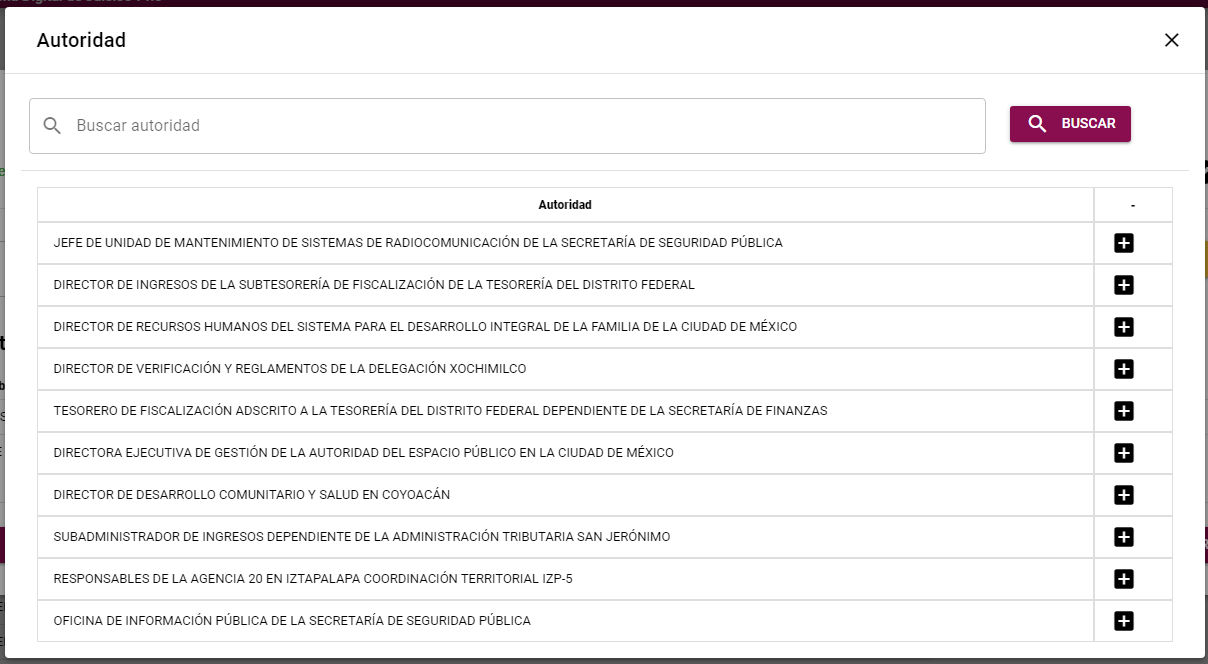
\includegraphics[width=0.90\columnwidth]{auto1.png}
\end{center}

Podemos dar click en el botón + para agregarla o buscarla y dar click en el botón {\bf{<<buscar>>}}
para después dar click en el botón + y agregarla y nos aparecerá en Autoridades

\begin{center}
    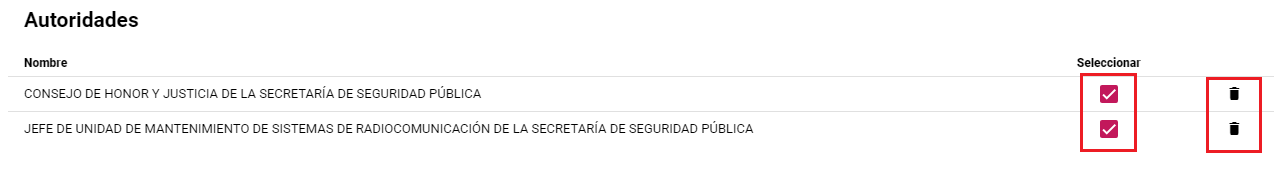
\includegraphics[width=0.90\columnwidth]{auto2.png}
\end{center}

Daremos click en (c) {\bf{<<seleccionar>> }}
o bien (d) Eliminar  si lo requerimos.\\
Después daremos click en el botón  \includegraphics[width=.15\columnwidth]{GUARDAR.png}

{\Huge{\color{myblue} \section{Borrar}\label{sec:20}}}
Podemos borrar la notificación dando click en el icono (3).

{\Huge{\color{myblue} \section{Más}\label{sec:21}}}
La opción Más (4) nos ofrece las siguientes opciones:

\begin{center}
    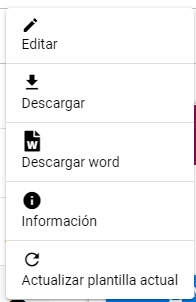
\includegraphics[width=0.20\columnwidth]{mas_cedulas.png}
\end{center}

{\bf{ <<Editar notificación>>}} Nos permite editar la notificación
\begin{center}
    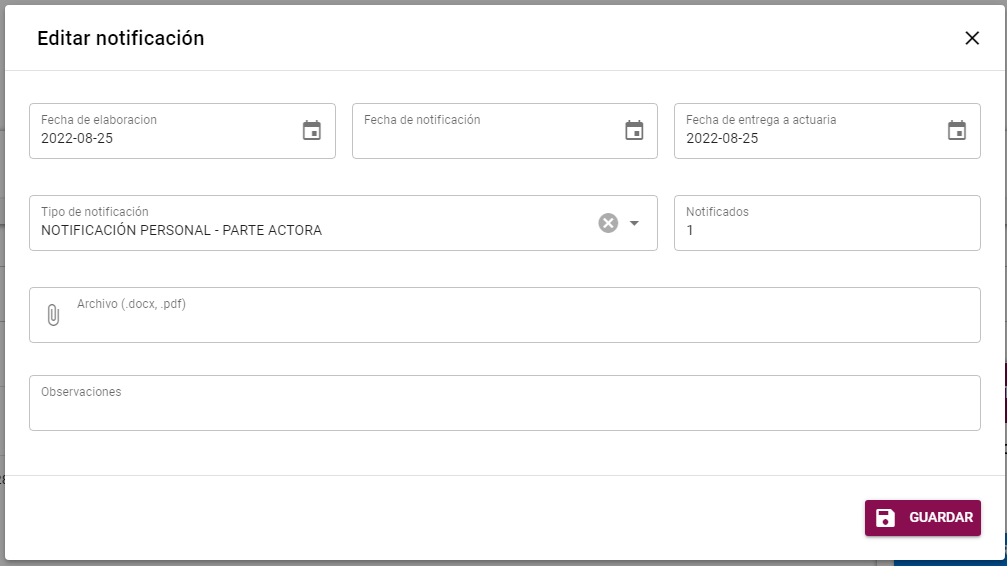
\includegraphics[width=0.70\columnwidth]{edi_noti.png}
\end{center}

{\bf{ <<Descarga>>}}
Esta opción nos permite descargar a nuestro equipo el archivo en formato pdf.\\

{\bf{ <<Descargar en word>>}}
Esta opción nos permite descargar a nuestro equipo el archivo en formato word.\\
{\bf{ <<Información>>}}
Esta opción nos permite ver detalles de la cédula.\\

\begin{center}
    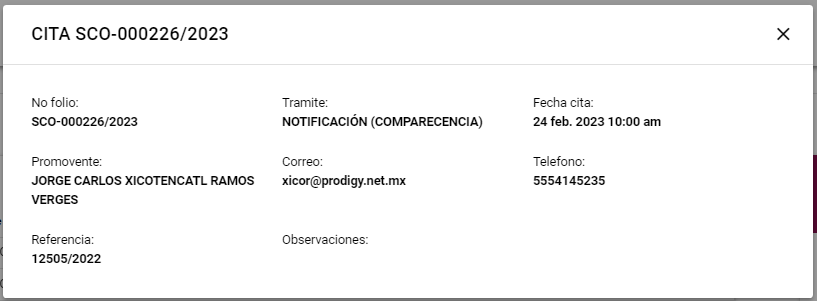
\includegraphics[width=0.70\columnwidth]{inf.png}
\end{center}

{\bf{<<Actualizar plantilla>>}} Nos permite actualizar la plantilla a la versión más reciente, daremos click en  {\bf{ <<Actualizar>>}}
\begin{center}
    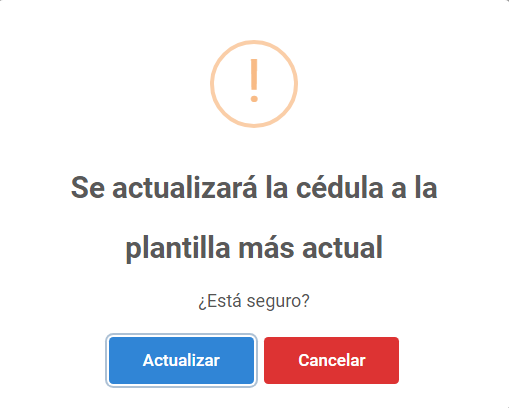
\includegraphics[width=0.40\columnwidth]{alet.png}
\end{center}

{\Huge{\color{myblue} \section{Borrar listado}\label{sec:22}}}
Para borrar el listado daremos click en el botón     

\includegraphics[width=.15\columnwidth]{borrarlist.png} y nos aparecerá la siguiente pantalla

\begin{center}
    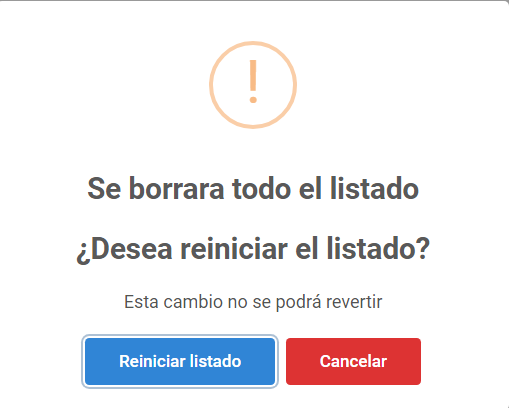
\includegraphics[width=0.50\columnwidth]{blist.png}
\end{center} 

daremos click en Reiniciar listado.

{\Huge{\color{myblue} \section{Imprimir listado}\label{sec:23}}}

Para imprimir un listado tenemos que dar click en el botón.


\includegraphics[width=0.15\columnwidth]{imprilist.png} nos 
abrirá una nueva pagina donde daremos click en el botón imprimir.


\chapter{\large{Administración -  Plantillas v1.0.1}}\label{}

En esta sección de Administración de plantillas podrás realizar las siguientes actividades:

\begin{itemize}
    \item Búsqueda de carpeta.
    \item Añadir carpeta.
    \item Agregar permisos.
    \item Información.
    \item Editar.
    \item Eliminar.
    \item Registro de carpeta de plantillas.
\end{itemize}


{\Huge{\color{myblue} \section{¿Cómo buscar carpeta?}\label{sec:24}}}
Para hacer la búsqueda de una carpeta, ingresaremos el nombre en la siguiente pantalla y daremos click en el botón {\bf{ <<Buscar>>}}

\begin{center}
    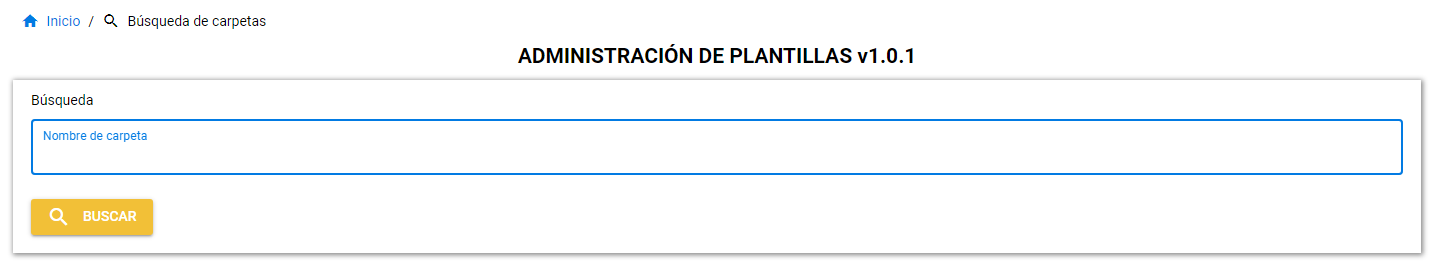
\includegraphics[width=0.90\columnwidth]{buscarc.png}
\end{center}

{\Huge{\color{myblue} \section{¿Cómo agregar una carpeta?}\label{sec:25}}}

\begin{center}
    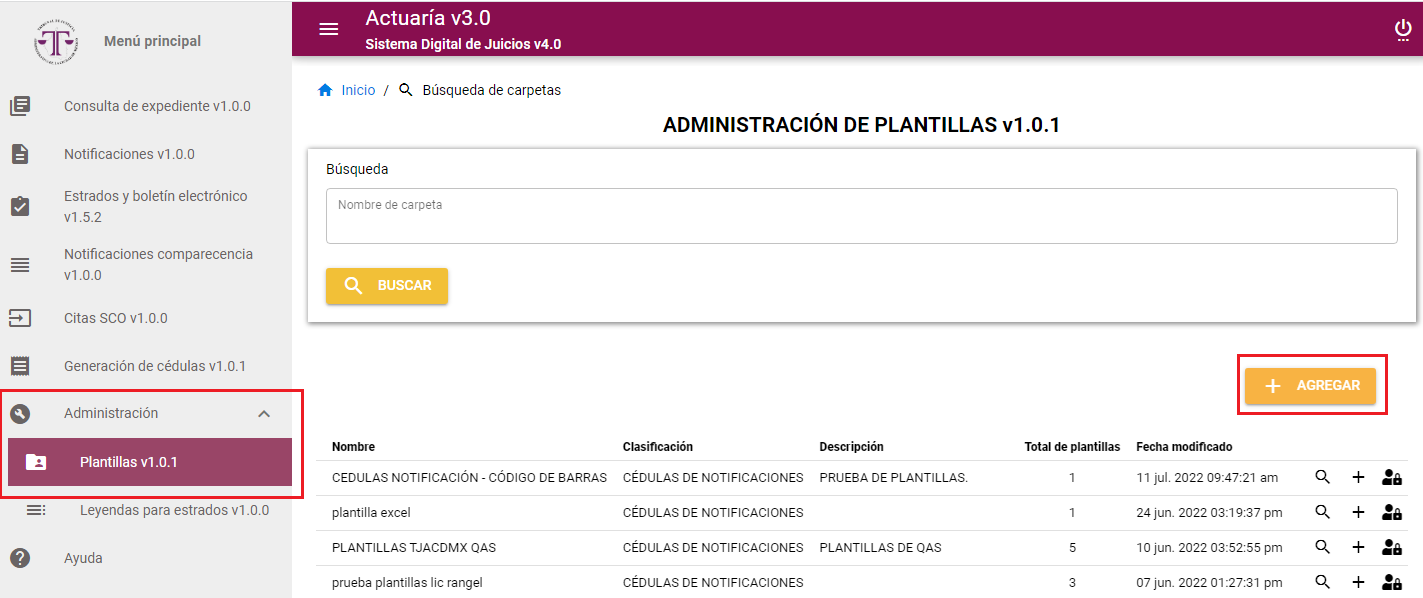
\includegraphics[width=0.90\columnwidth]{plantilla3.png}
\end{center}

Para añadir una plantilla nos ubicaremos en {\bf{ <<Plantillas v1.0.1>>}}
y daremos click en el botón {\bf{ << + AGREGAR>>}} \\
Automáticamente nos aparecerá la siguiente pantalla:

\begin{center}
    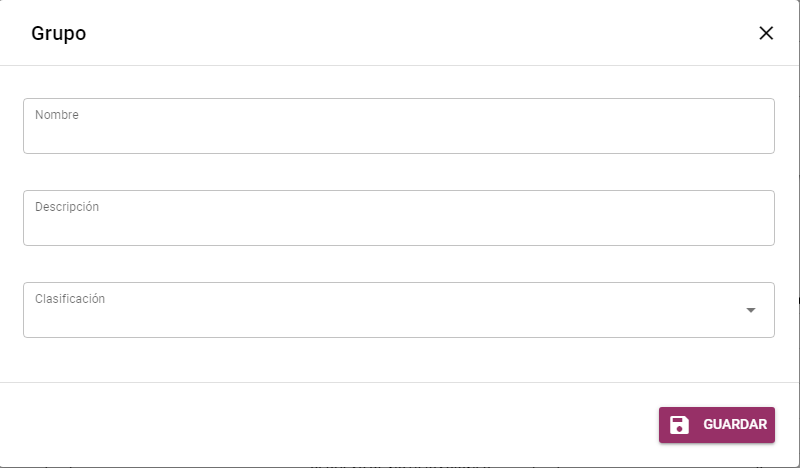
\includegraphics[width=0.50\columnwidth]{GRUPO.png}
\end{center}

Ingresaremos los siguientes datos:
\begin{itemize}
    \item Nombre
    \item Descripción
    \item Clasificación
\end{itemize}

Y daremos click en el botón {\bf{ <<GUARDAR>>}}

{\Huge{\color{myblue} \section{Iconos}\label{sec:26}}}
\begin{center}
    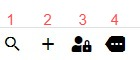
\includegraphics[width=0.30\columnwidth]{iconos.jpeg}
\end{center}
Podemos realizar las siguientes acciones:

\begin{enumerate}[(1)]
    \item Consultar
    \item Añadir plantilla +
    \item Agregar permisos
    \item Mas 
    \begin{itemize}
        \item Información.
        \item Editar.
        \item Eliminar
    \end{itemize}
\end{enumerate}

{\Huge{\color{myblue} \section{Consultar}\label{sec:27}}}

Para consultar carpeta de plantillas dar click  en el icono     
\includegraphics[width=0.05\columnwidth]{lupa.png}
y nos mostrará la siguiente pantalla.

Dónde podemos observar:


{\color{myblue}
\begin{itemize}
    \item Nombre de carpeta.
    \item Clasificación.
    \item Propietario (Creador de la carpeta).
    \item Fecha de creación.
    \item Listado de las plantillas creadas
\end{itemize}
}
\begin{center}
    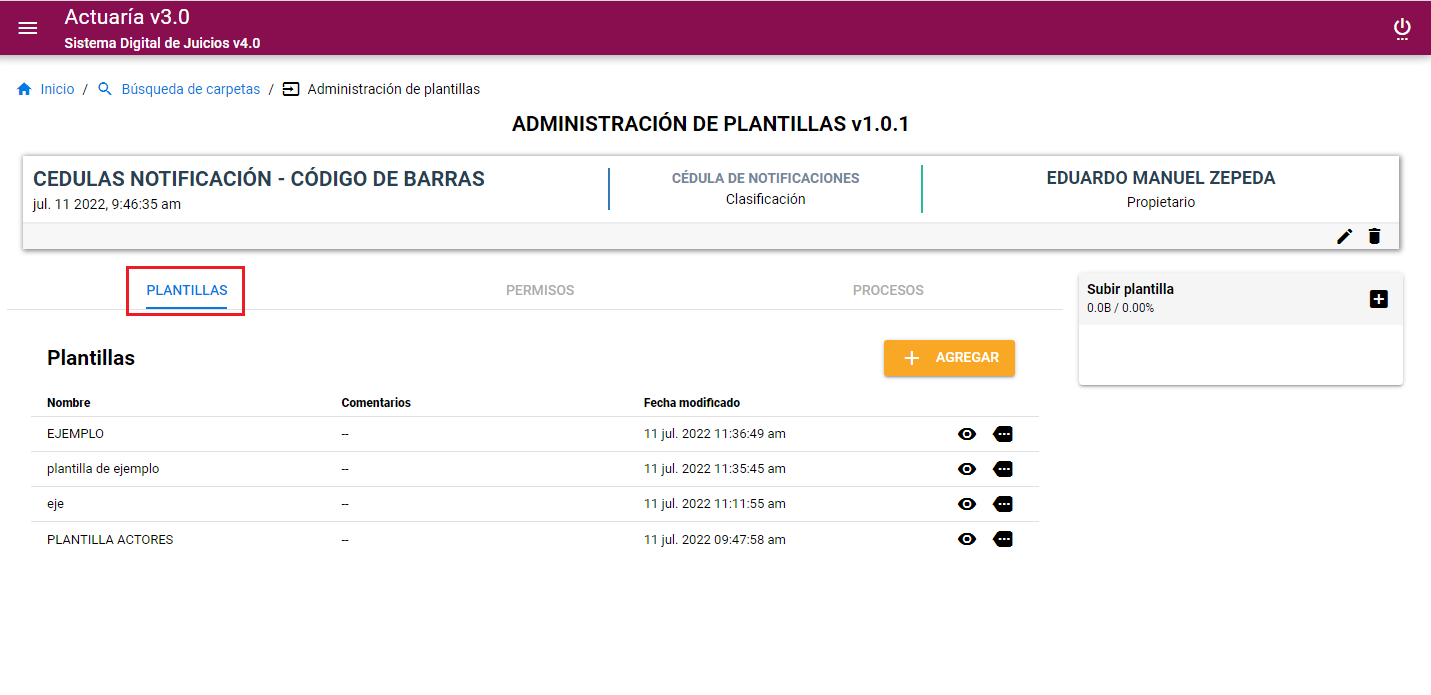
\includegraphics[width=0.90\columnwidth]{adminp.png}
\end{center}

Podemos {\bf{ <<Subir plantilla>>}} dando click en el botón +

\begin{center}
    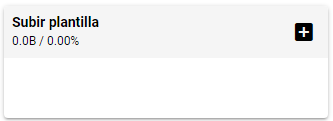
\includegraphics[width=0.50\columnwidth]{subir.png}
\end{center}


Seleccionando desde nuestros archivos la plantilla deseada y damos click en {\bf{ <<Abrir>>}}

\begin{center}
    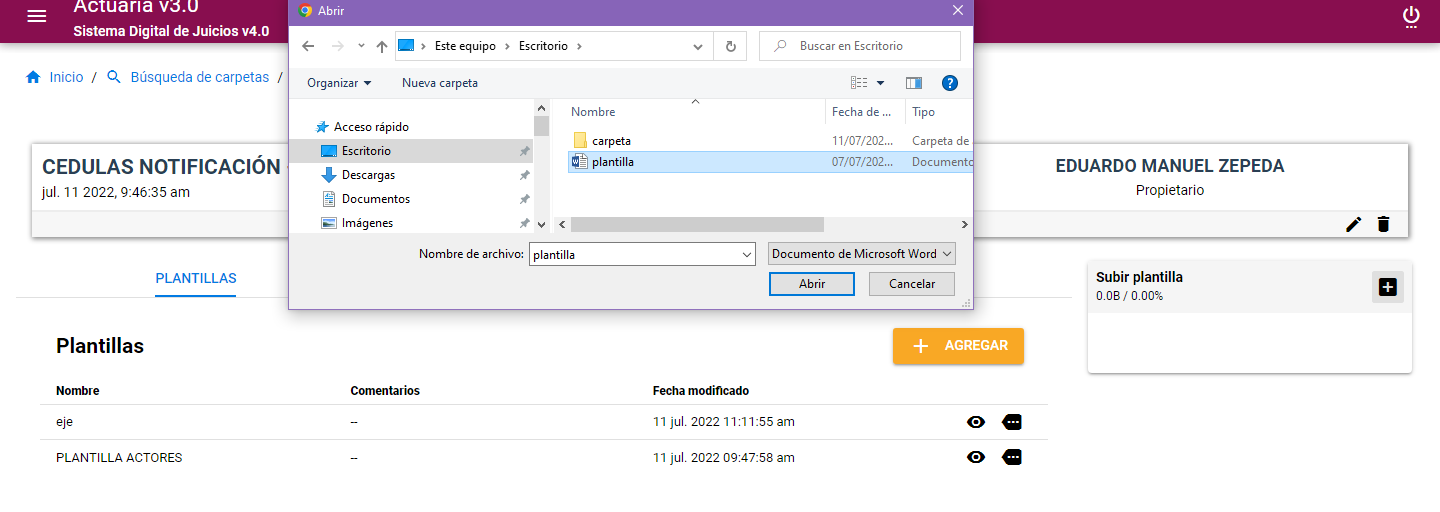
\includegraphics[width=0.90\columnwidth]{plantilla4.png}
\end{center}

Nos aparecerá la siguiente pantalla e ingresaremos los datos de la plantilla y daremos click en {\bf{ <<GUARDAR>>}}

\begin{center}
    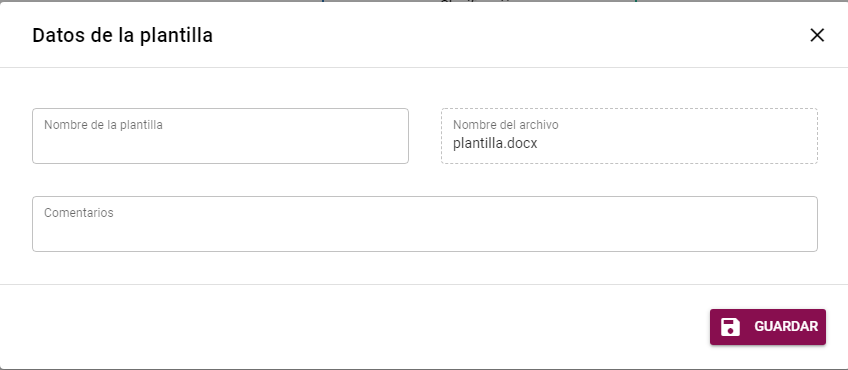
\includegraphics[width=.50\columnwidth]{datosp.png}
\end{center}


De igual forma podemos utilizar el botón 
\includegraphics[width=.15\columnwidth]{agregar.png} para agregar una plantilla.
Dando click en el nos mostrará la pantalla para ingresar los datos de la plantilla, seleccionar el archivo 
desde nuestros documentos.

\begin{center}
    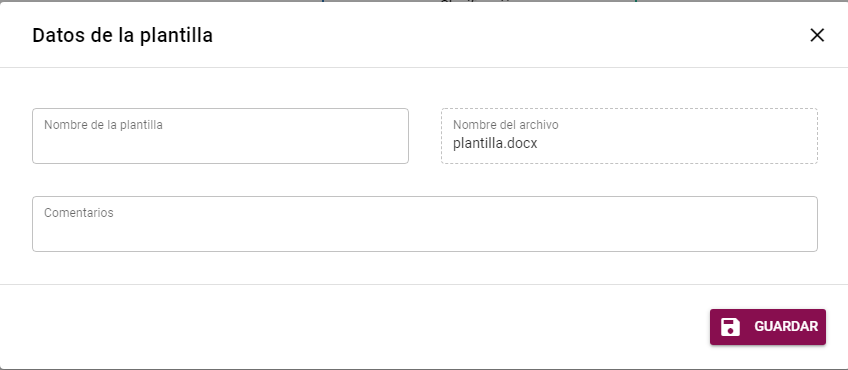
\includegraphics[width=.50\columnwidth]{datosp.png}
\end{center}

A continuación, se enlistan las variables disponibles:
\begin{itemize}
\item \$SALA\$
\item \$PONENCIA\$
\item \$NOJUICIO\$
\item \$ACTUACION\$
\item \$ACTOR\$
\item \$ACTUARIO\$
\item \$AUTORIDADES\$
\item \$TERCEROS\$
\item \$ACTORES\$
\item \$RA\$
\item \$RRC\$
\item \$FECHA\_ELABORACION\_CEDULA\$
\item \$AUTORIZADOS\$
\item \$DOMICILIO\_NOTIFICACIONES\$
\item \$TIPO\_ACUERDO\$
\item \$FECHA\_ACUERDO\$
\end{itemize}

El formato definido en el texto que compone la variable, será respetado por el sistema; por ejemplo,
Negrita, Cursiva y Subrayado:\\
\begin{itemize} 
\item {{\bf\$PONENCIA\$ }} \\
\item  \textit{\$DOMICILIO\_NOTIFICACIONES\$}\\
\item \underline{\$ACTUARIO\$} \\
\end{itemize}

Ejemplo de cédula:
\begin{center}
    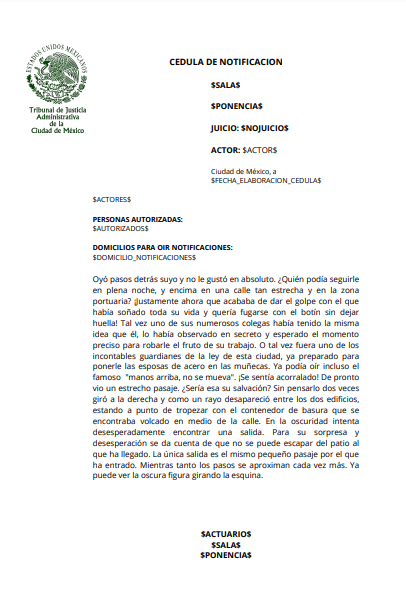
\includegraphics[width=0.80\columnwidth]{cedula.png}
\end{center}

Para cada plantilla podemos realizar las siguientes acciones:
\begin{center}
    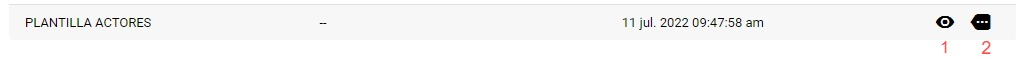
\includegraphics[width=.88\columnwidth]{accionp.jpeg}
\end{center}

\begin{enumerate}[1.]
    \item Visualizar
    \item Más
\end{enumerate}

Para visualizar el documento daremos click en el icono     
\includegraphics[width=.05\columnwidth]{ojo.png}
Y nos aparecerá nuestra plantilla.
\begin{center}
    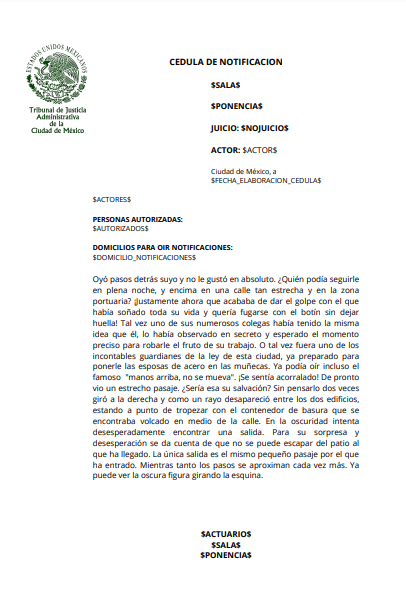
\includegraphics[width=.55\columnwidth]{cedula.png}
\end{center}

La opción {\bf{ <<Más>>}} nos ofrece lo siguiente:\\
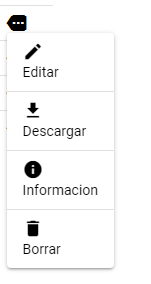
\includegraphics[width=.20\columnwidth]{mas3.png}

La opción {\bf{ <<Editar>>}} nos permite editar los datos de nuestra plantilla, dando click en     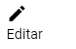
\includegraphics[width=.10\columnwidth]{edi.png}, nos aparecerá la siguiente pantalla.
\begin{center}
    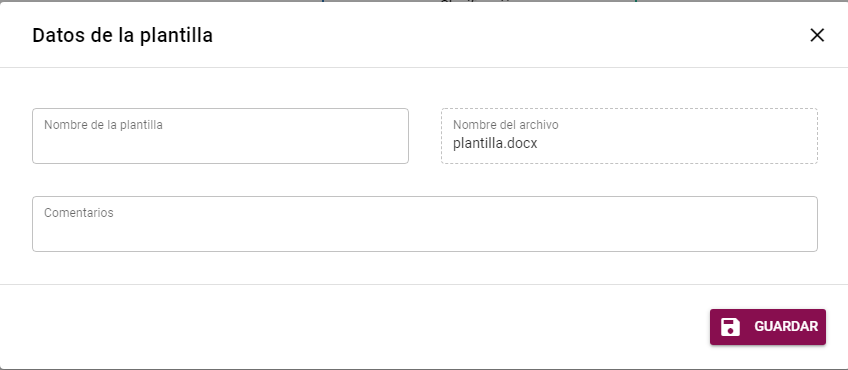
\includegraphics[width=.50\columnwidth]{datosp.png}
\end{center}

Después de editar nuestros datos deseados daremos click en el botón {\bf{ <<GUARDAR>>}}
\vspace{1cm}

La opción {\bf{ <<Descargar>>}} nos permite descargar nuestra plantilla y guardarla en nuestro equipo, para hacerlo daremos click en la opción     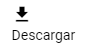
\includegraphics[width=.10\columnwidth]{desc.png} y seleccionaremos donde queremos que se guarde.
\begin{center}
    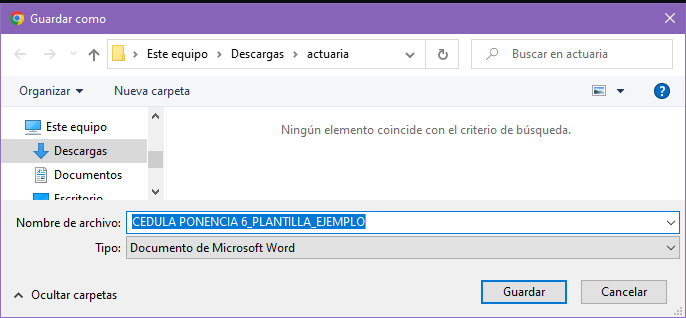
\includegraphics[width=.88\columnwidth]{descargar.png}
\end{center}

Posteriormente se iniciará la descarga en nuestro equipo.
\begin{center}
    
\includegraphics[width=.88\columnwidth]{descargar1.png}
\end{center}

La opción {\bf{ <<información >>}} nos permite ver la información de nuestra plantilla, dando click en  
\includegraphics[width=0.10\columnwidth]{infor.png} y nos aparecerá la información

\begin{center}
    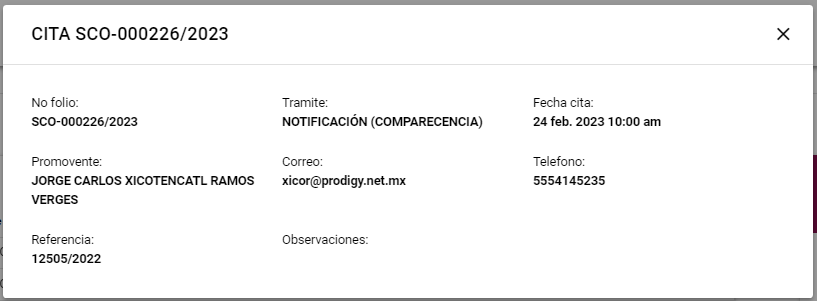
\includegraphics[width=0.8\columnwidth]{inf.png}
\end{center}

Con la opción {\bf{<<Borrar>>}} podremos borrar nuestra plantilla, dando click en
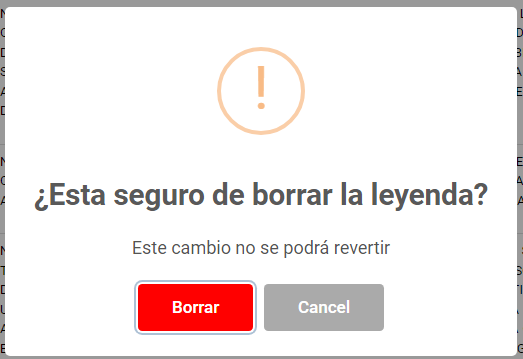
\includegraphics[width=.10\columnwidth]{borrar.png}
nos aparecerá el siguiente mensaje

\begin{center}
    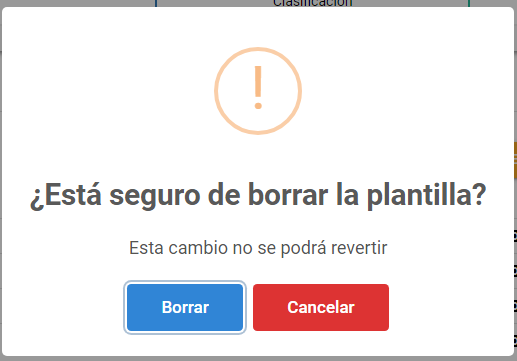
\includegraphics[width=.50\columnwidth]{borrarp.png}
\end{center}
    Daremos click en <<Borrar>>

\vspace{1cm}

En la opción {\bf{ PERMISOS}}

\begin{center}
    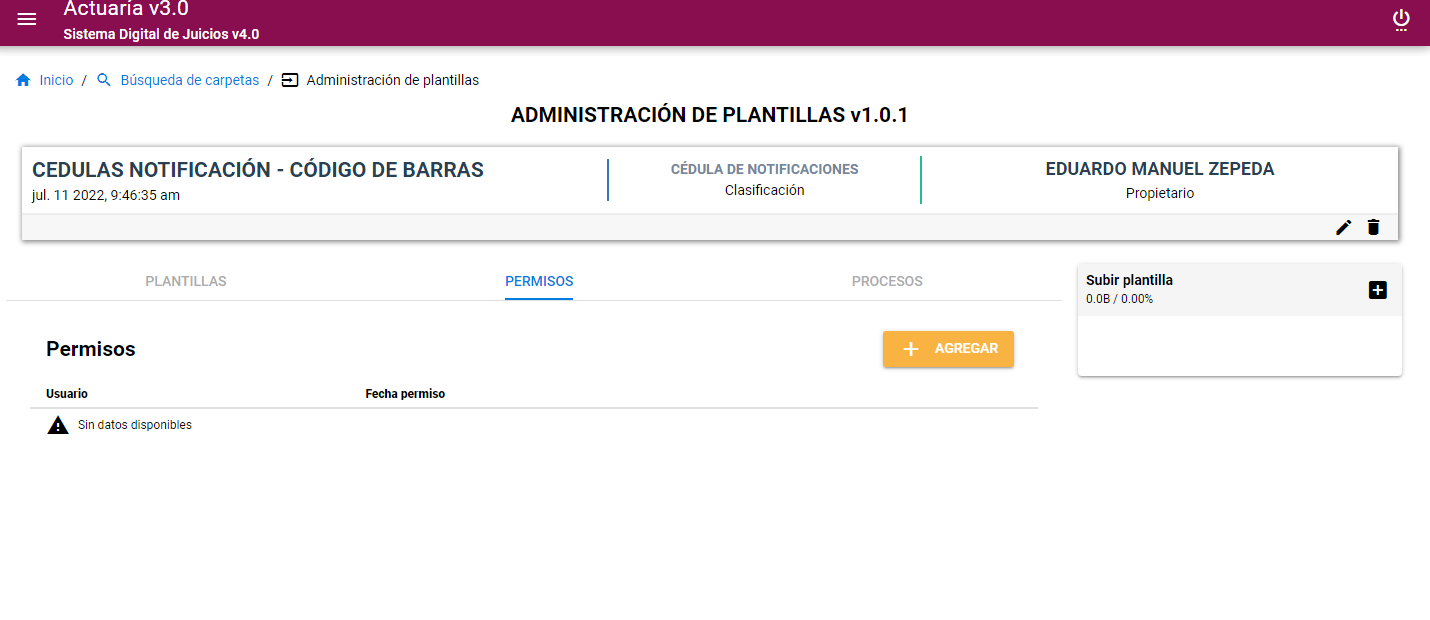
\includegraphics[width=0.88\columnwidth]{permi1.png}
\end{center}

Podemos agregar nuevos permisos, dando click en el botón     
\includegraphics[width=.15\columnwidth]{agregar.png}, nos aparecerá la siguiente pagina:

\begin{center}
    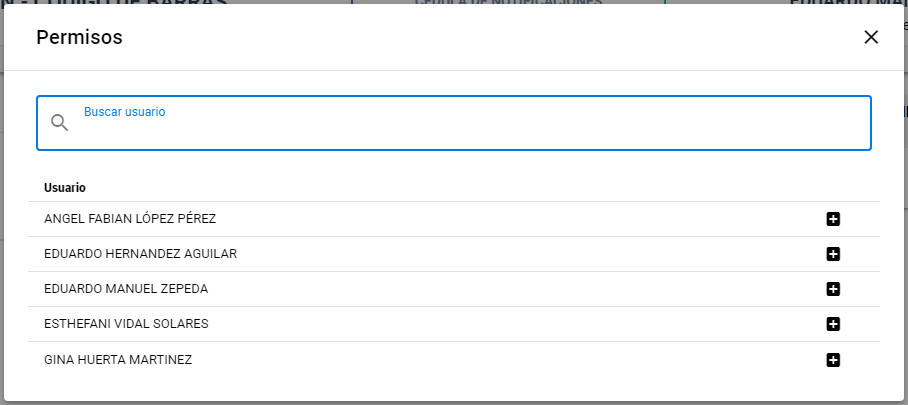
\includegraphics[width=0.88\columnwidth]{permi2.png}
\end{center}

Podemos buscar o seleccionar al usuario con el botón + y automáticamente se agregara mostrando el siguiente mensaje.

\begin{center}
    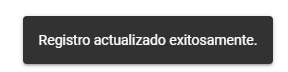
\includegraphics[width=0.30\columnwidth]{permi3.png}
\end{center}

También podemos eliminar el usuario dando click en el icono     
\includegraphics[width=0.05\columnwidth]{iconob.png}, nos aparecerá el siguiente mensaje:

\begin{center}
    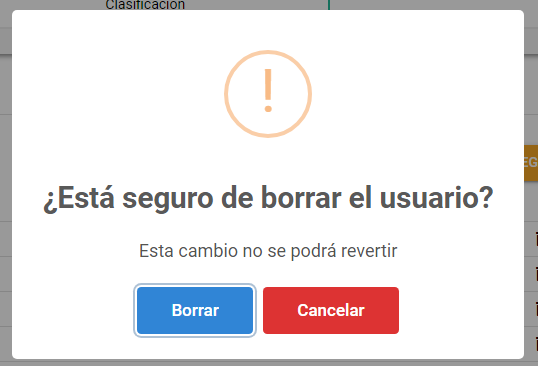
\includegraphics[width=.50\columnwidth]{busuario.png}
\end{center}

Daremos click en {\bf{ <<Borrar>>.}}
\vspace{1cm}

En la opción {\bf{ PROCESOS}}

\begin{center}
    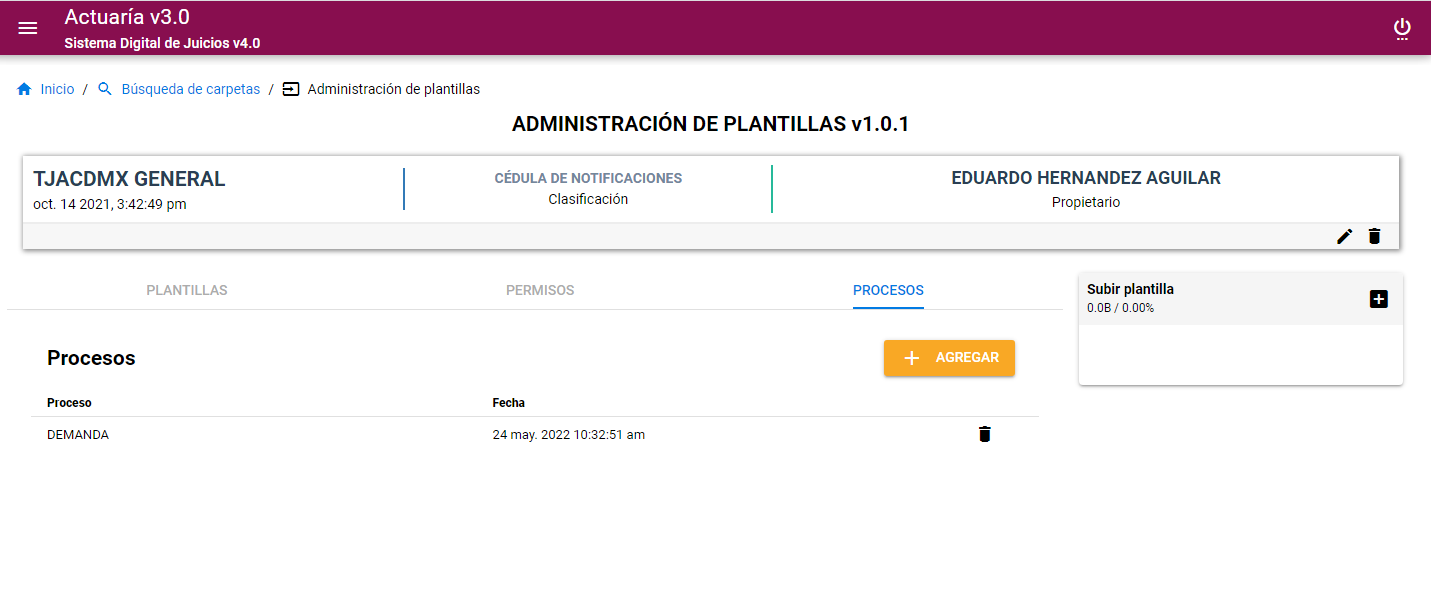
\includegraphics[width=.88\columnwidth]{proc1.png}
\end{center}

Podemos agregar procesos dando click en el botón   
\includegraphics[width=.15\columnwidth]{agregar.png}, nos aparecerá la siguiente pagina

\begin{center}
    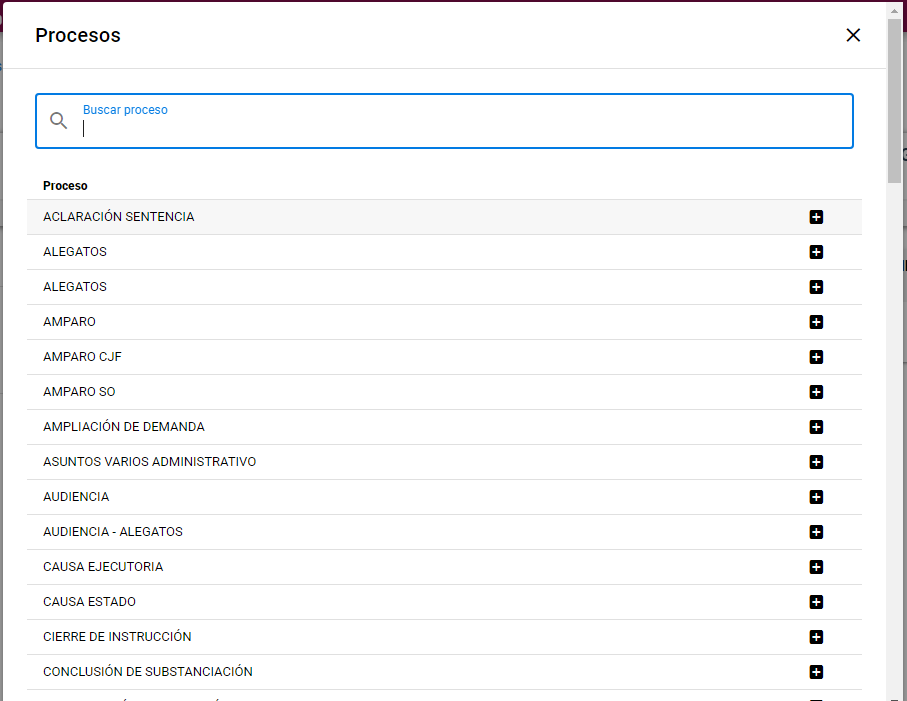
\includegraphics[width=.88\columnwidth]{proc2.png}
\end{center}

Elegiremos los procesos que deseemos dando click en el +  y automáticamente  se registrara.

\begin{center}
    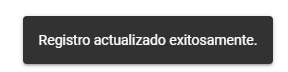
\includegraphics[width=.50\columnwidth]{permi3.png}
\end{center}

Podemos borrar el proceso dando click en el icono    
\includegraphics[width=.05\columnwidth]{iconob.png} y nos aparecerá el siguiente mensaje

\begin{center}
    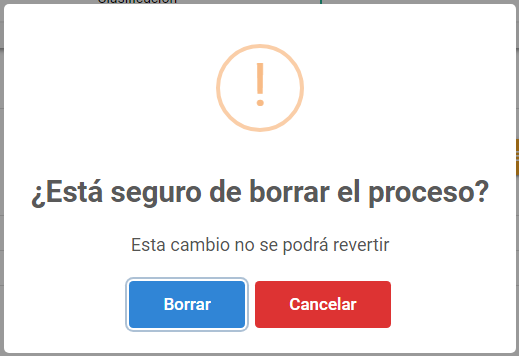
\includegraphics[width=.50\columnwidth]{bproceso.png}
\end{center}

Elegiremos la opción Borrar.
\vspace{1.0 cm}
{{\bf
(2) Añadir plantilla}}
utilizando el icono +

\begin{center}
    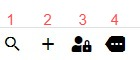
\includegraphics[width=.40\columnwidth]{iconos.jpeg}
\end{center}

Daremos click en el icono + y nos aparecerá la siguiente pantalla:

\begin{center}
    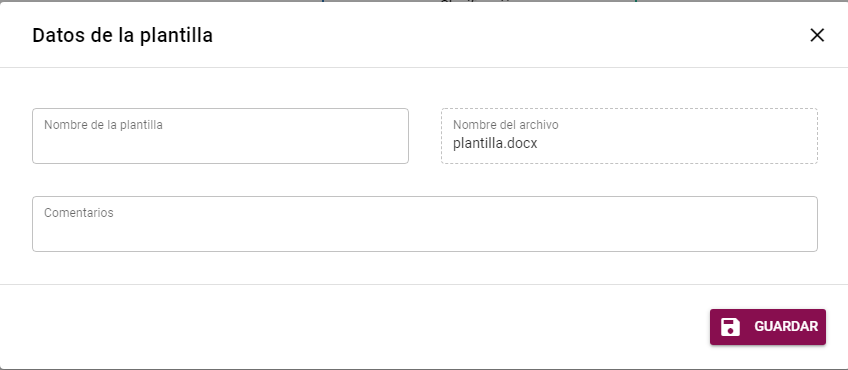
\includegraphics[width=.88\columnwidth]{datosp.png}
\end{center}

Ingresaremos los datos de la plantilla, y seleccionaremos
el archivo desde nuestros documentos.

\begin{center}
    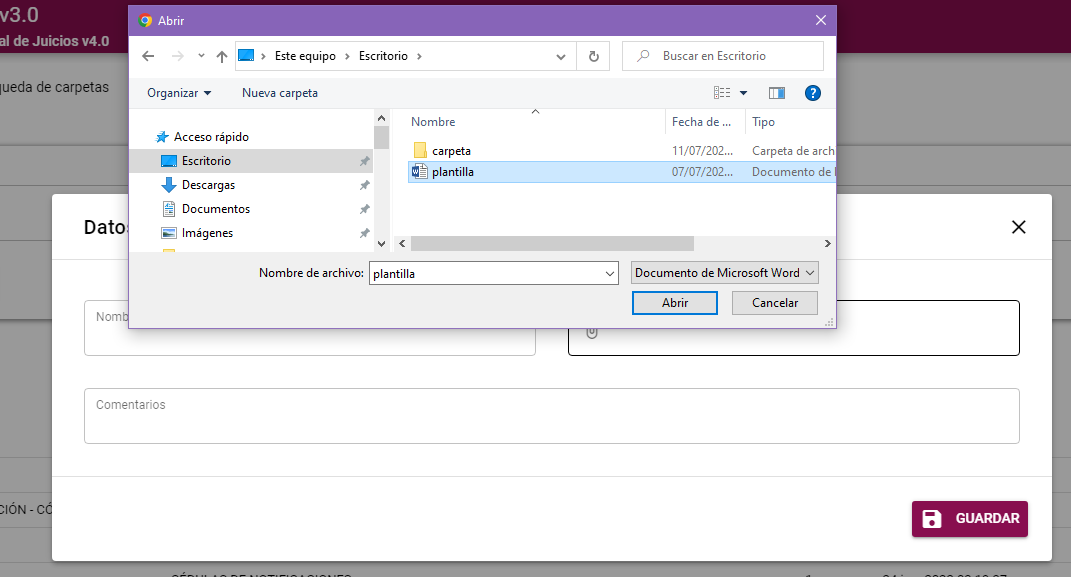
\includegraphics[width=.88\columnwidth]{plantilla10.png}
\end{center}

Daremos click en <<Abrir>> , el sistema agregara el archivo y daremos click en el botón  {{\bf
<<GUARDAR>>}}


{{\bf (3) Agregar permisos}}\\
Daremos click en el icono     
\includegraphics[width=.05\columnwidth]{permisos2.png}
y nos aparecerá la siguiente pantalla:

\begin{center}
    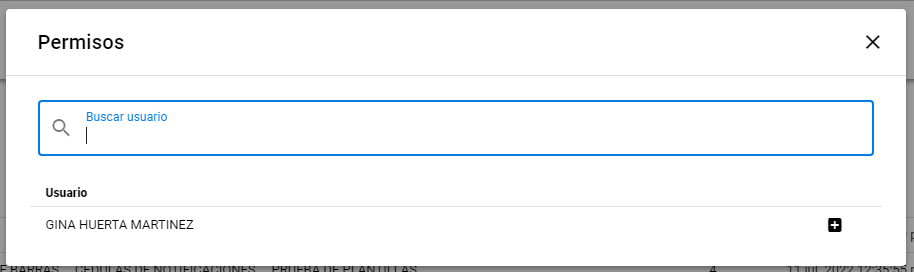
\includegraphics[width=.88\columnwidth]{permi6.png}
\end{center}

Seleccionares la opción deseada con el icono +
Y automáticamente se registrara en el sistema, mostrado el siguiente mensaje.

\begin{center}
    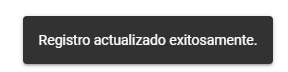
\includegraphics[width=.30\columnwidth]{permi3.png}
\end{center}

Ingresaremos los datos de la plantilla, y seleccionaremos
el archivo desde nuestros documentos.

{{\bf (4) Más}}\\El icono

\includegraphics[width=.05\columnwidth]{mas2.png}
nos ofrece  las siguientes opciones:

\begin{center}
    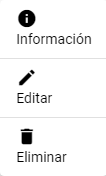
\includegraphics[width=.15\columnwidth]{mas10.png}
\end{center}

La opción     
\includegraphics[width=.10\columnwidth]{infor.png}
nos permite ver la información de la carpeta
dando click .

\begin{center}
    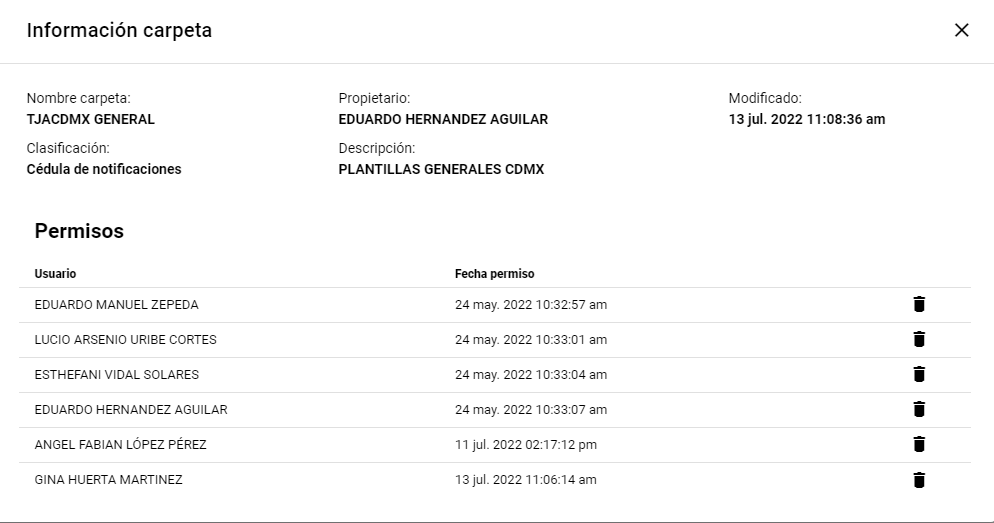
\includegraphics[width=.88\columnwidth]{incarpeta.png}
\end{center}

Podemos ver:
\begin{itemize}
    \item Nombre carpeta
    \item Propietario
    \item Modificación
    \item Clasificación
    \item Descripción
    \item Permisos
\end{itemize}

Y oportunidad de borrar permisos dando click en el icono

\includegraphics[width=.05\columnwidth]{iconob.png}\\
La opción     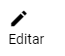
\includegraphics[width=.10\columnwidth]{editar10.png}
nos permite editar el grupo.
Para ello daremos click y nos aparecerá la siguiente pantalla:

\begin{center}
    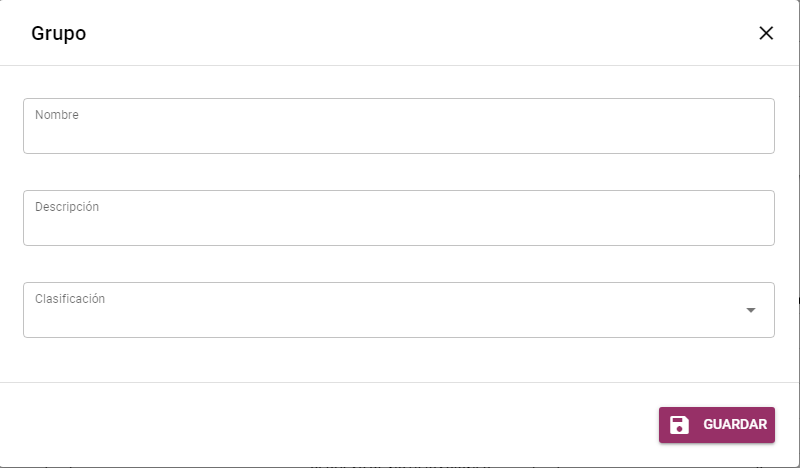
\includegraphics[width=.50\columnwidth]{GRUPO.png}
\end{center}

Podemos editar:
\begin{itemize}
    \item Nombre
    \item Descripción
    \item Clasificación
\end{itemize}

Después de editar lo deseado daremos click en el botón {{\bf
<<GUARDAR>>}}

La opción     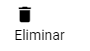
\includegraphics[width=.10\columnwidth]{eliminar.png}
nos permite eliminar el grupo.\\
Para ello daremos click y nos aparecerá el siguiente mensaje:

\begin{center}
    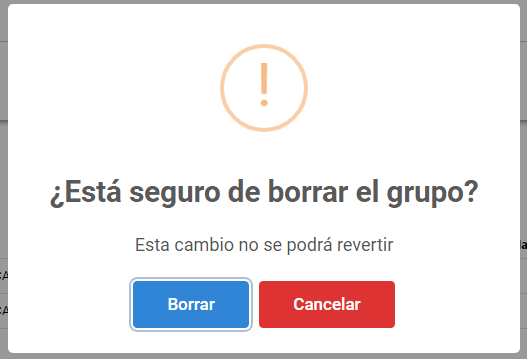
\includegraphics[width=.50\columnwidth]{eligrupo.png}
\end{center}

Daremos click en el botón {\bf{<<Borrar>>}}


\chapter{\large{Administración de Leyendas v1.0.0}}\label{chap:leyendas}
En este módulo podemos:
\begin{enumerate}[(1)]
    \item Buscar leyenda
    \item Registrar leyenda
    \item Editar leyenda
    \item Borrar leyenda
\end{enumerate}

\begin{center}
    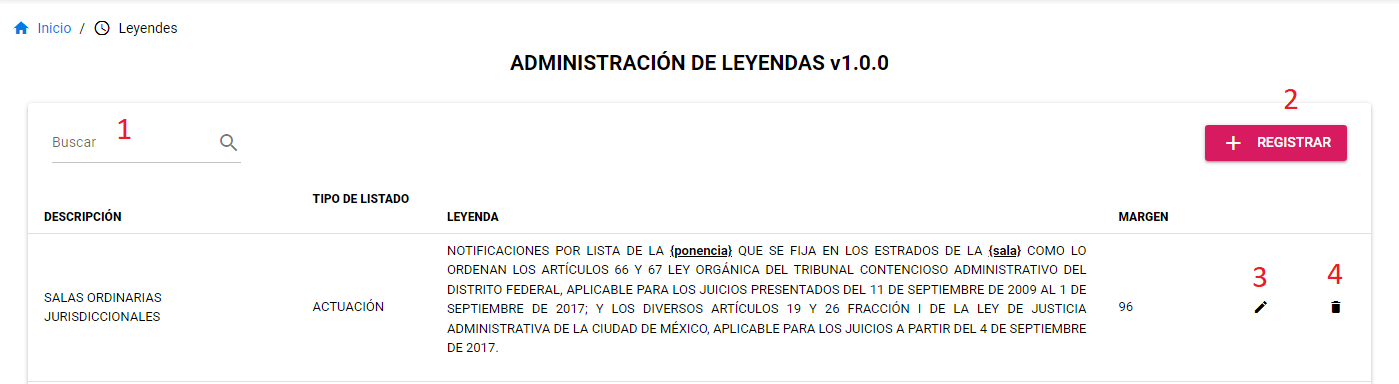
\includegraphics[width=0.90\columnwidth]{leyendas.png}
\end{center}

{\Huge{\color{myblue} \section{Buscar leyenda}\label{sec:28}}}

Para buscar una leyenda bastará con ingresar el texto en el buscador que se encuentra de lado superior izquierdo, identificado con el número 1.  \textit{Ver ~\nameref{chap:leyendas}}\\

{\Huge{\color{myblue} \section{ Registrar leyenda}\label{sec:29}}}

Para registrar una leyenda de click sobre el botón {\bf{<<REGISTRAR>>}}
se mostrará una pantalla con los siguientes datos.

\begin{center}
    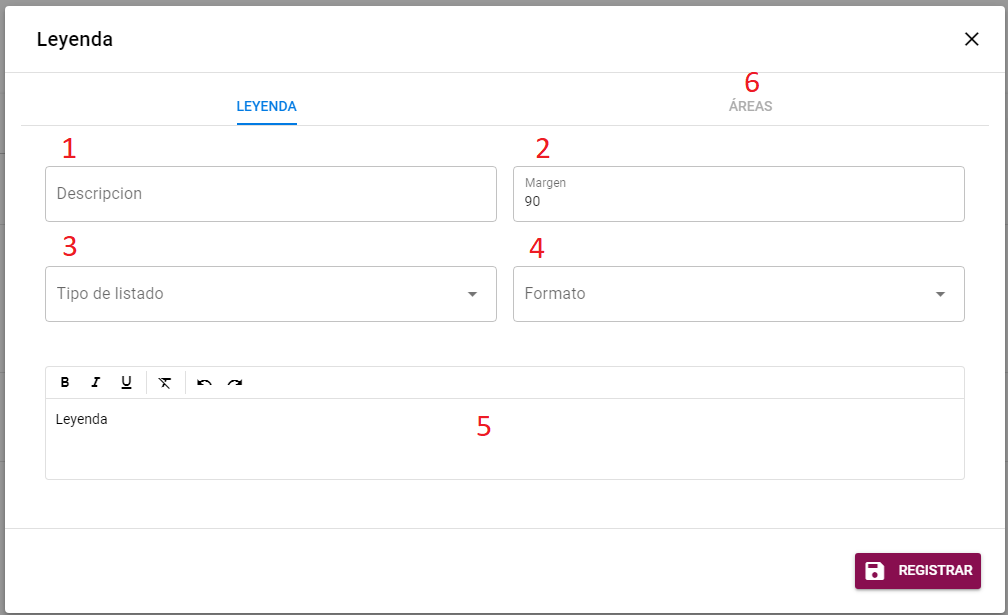
\includegraphics[width=0.77\columnwidth]{leyenda_datos.png}
\end{center}

Ingresa:
\begin{enumerate}
    \item Descripción
    \item Margen
    \item Tipo de listado
    \item Formato
    \item Leyenda
    \item Áreas
\end{enumerate}

Posteriormente da click en el botón {\bf{<<GUARDAR>>}}

{\Huge{\color{myblue} \section{Editar leyenda}\label{sec:30}}}

Para editar una leyenda bastará con dar click sobre el icono {\bf{ <<Editar>>}} que se encuentra de lado derecho, identificado con el número 3   \textit{Ver ~\nameref{chap:leyendas}}\\
Edite los datos deseados y de click en el botón actualizar

\begin{center}
    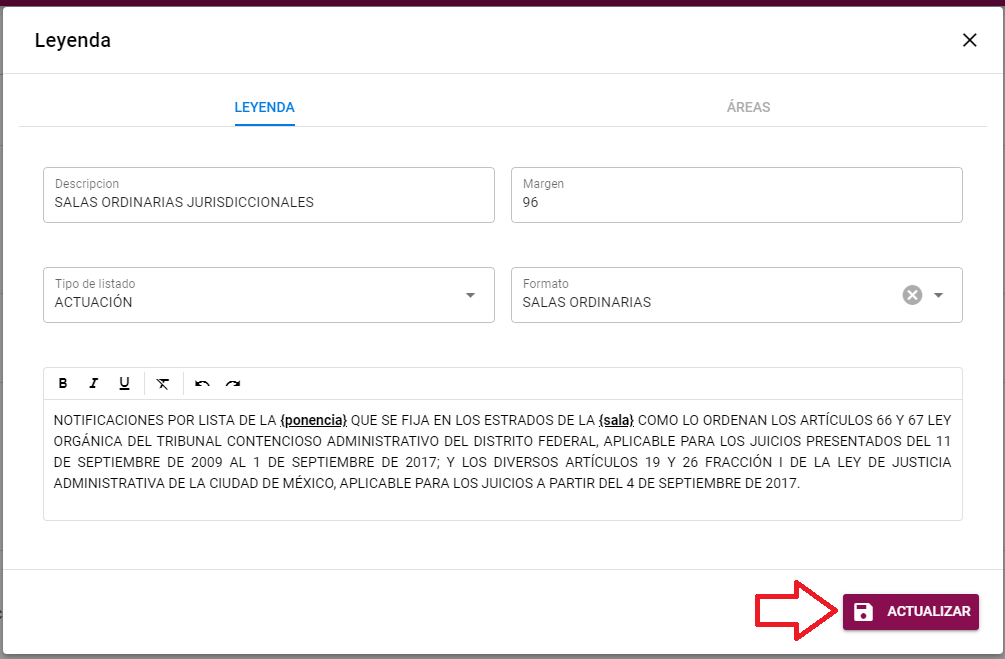
\includegraphics[width=0.77\columnwidth]{actualizar.png}
\end{center}


{\Huge{\color{myblue} \section{Borrar leyenda}\label{sec:30.1}}}

Para borrar una leyenda bastará con dar click sobre el icono {\bf{ <<Borrar>>}} que se encuentra de lado derecho, identificado con el número 4   \textit{Ver ~\nameref{chap:leyendas}}\\
Se mostrará un mensaje de advertencia, da click en el botón aceptar.


\begin{center}
    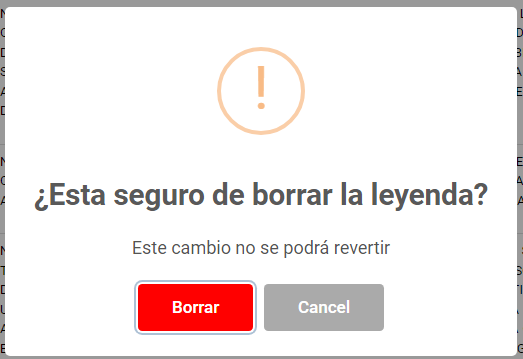
\includegraphics[width=0.44\columnwidth]{borrar.png}
\end{center}

\end{document}
